%\setcounter{section}{0}
%\setcounter{subsection}{0}
%\setcounter{subsubsection}{0}
%\setcounter{equation}{0}
%\pagenumbering{arabic} 
%\setcounter{page}{0}    %%%%%KKD used \setcounter{page}{0}  
%\oddsidemargin 0.9 cm 
%\evensidemargin -.4 cm
%\setlength{\textwidth}{152.4 mm}





\chapter{Search for Supersymmetry with 13 TeV pp Collision Data  \label{Search for Supersymmetry with 13 TeV pp Collision Data}}

As discusssed earlier, SUSY is one BSM theory that provides solutions to the problems of the SM. It provides a way to cancel the Higgs mass divergence problem, to unify strong, weak and electromagnetic interactions, and has a candidate for dark matter. Natural SUSY models~\cite{Naturaln} minimize the fine tuning associated with the value of the Higgs boson mass and its radiative corrections. In these models, the top squark, left-handed bottom squark, gluino, and higgsino are required to be light, i.e., to have masses near the electroweak energy scale, making them potentially accessible at the LHC. Among many SUSY processes, the gluino pair production has largest cross-section~\cite{xsecGlu} which increases the order of 30 going from 8 TeV to 13 TeV. This fact makes it pertinent to search for SUSY even with a couple of $\rm fb^{-1}$ of data. Since baryon number and lepton number conservation have been tested very precisely, these couplings need to be very small in order not to be in conflict with experimental data. R-parity is a symmetry acting on the Minimal Supersymmetric Standard Model (MSSM) fields that forbids these couplings. In R-parity conserving SUSY models, the lightest supersymmetric SUSY particle is stable and a possible dark matter candidate. The results of our search are interpreted with R-parity~\cite{RParity} conserving simplified SUSY scenarios~\cite{SMS1}.

In this chapter, we first describe the study with 2.3 $\rm fb^{-1}$ of the 2015 data and later with 12.9 $\rm fb^{-1}$ of 2016 data. We search in all hadronic final states i.e., in the final states of jets and missing transverse momentum. All hadronic SUSY searches are especially interesting, because they often make up a large portion of branching fractions for typical signals and tend to be easily hidden in extensions to  SUSY models.

We present a general search for gluino pair production leading to final states with large missing transverse energy ($\rm p_{T}^{miss}$), large scalar sum of transverse energy ($\rm H_{T}$), large number of jets ($\rm N_{jet}$) and large number of b-tagged jets ($\rm N_{b-jet}$). The event diagrams of gluino pair production that we considered in our analysis are shown below. We shall focus more on the $Z\rightarrow \nu \bar{\nu} $ invisible background estimation as this is the part of the analysis where we have contributed to the most. 


\begin{figure}[H]
    \centering
    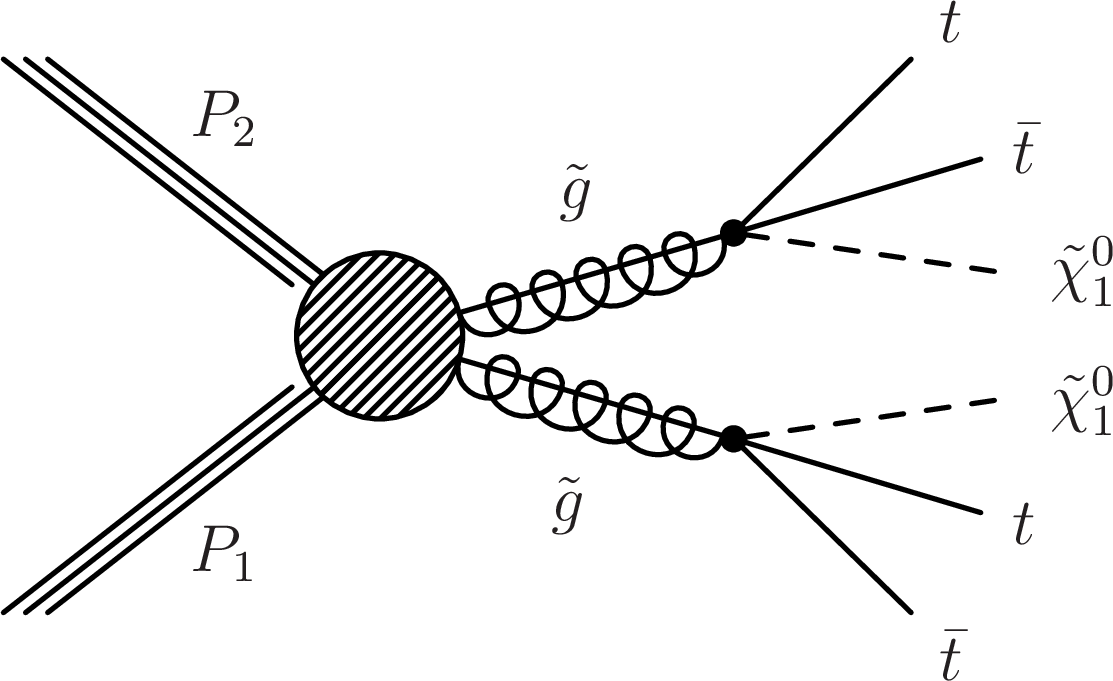
\includegraphics[width=5.0cm,height=4cm]{/home/bibhu/Desktop/PhDThesis/PhDThesis/chapter6/T1tttt.png}
    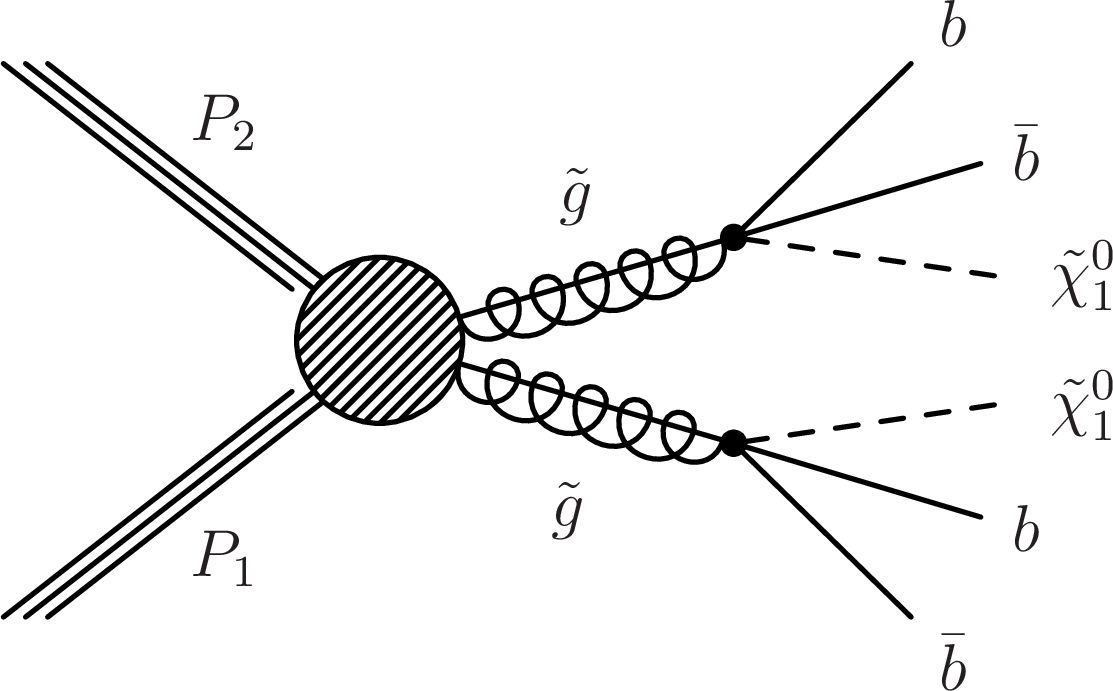
\includegraphics[width=5.0cm,height=4cm]{/home/bibhu/Desktop/PhDThesis/PhDThesis/chapter6/T1bbbb.png}
    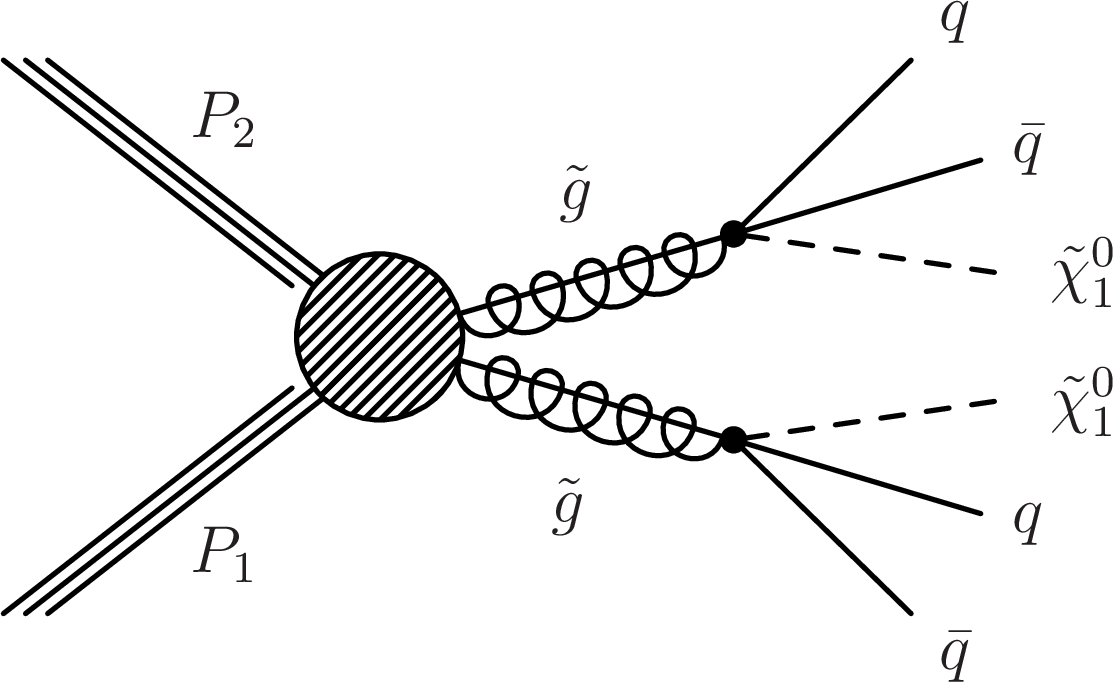
\includegraphics[width=5.0cm,height=4cm]{/home/bibhu/Desktop/PhDThesis/PhDThesis/chapter6/T1qqqq.png}
    \caption{ \small Event diagrams for gluino pair production with four top final state (left), four b-quark final state (middle) and four light quark final state (right)}
    \label{fig:SMSSUSYeventDiagrams}
\end{figure}


The major backgrounds for this final state come from $t\bar{t}$, w+jets ,Z($\rightarrow \nu\bar{\nu}$)+jets, QCD processes. All these backgrounds are estimated using data driven techniques, keeping usage of MC samples to a minimum. 

\section{Study with 2.3 $\rm fb^{-1}$ of the 2015 Data}

In this section, we shall describe the details of the SUSY search done with 2.3 $\rm fb^{-1}$ of the 2015 data.

\subsection{Data-MC samples and trigger}

MC samples that are used in the analysis are given in this section along with their cross sections. 
The SM samples are listed in Tables \ref{tab:signalMC}-\ref{tab:gjetsMCsamples}.  The cross
sections listed correspond to next-to-leading-order (NLO) calculations 
unless otherwise noted.  The samples correspond to a
pileup distribution with an average of 20 interactions per
bunch crossing and a 25 ns interval between bunches.

\begin{table}[h]
\centering
\caption{MC FullSim samples for signal SMS (Simplified SUSY Models) model points.}
\label{tab:signalMC}
{\footnotesize
\begin{tabular}{lccc}
\hline \hline
Dataset (masses in GeV ) & Generator & $\sigma$ (pb) & $(\rm fb^{-1})$ \\
\hline
SMS-T1tttt ($\rm m_{gluino}=1500, m_{LSP}=100$) & madgraph-pythia8 & 0.014 & 7268\\
SMS-T1tttt ($\rm m_{gluino}=1200, m_{LSP}=800$) & madgraph-pythia8 & 0.086 & 1719\\
SMS-T1bbbb ($\rm m_{gluino}=1500, m_{LSP}=100$) & madgraph-pythia8 & 0.014 & 3708\\
SMS-T1bbbb ($\rm m_{gluino}=1000, m_{LSP}=900$) & madgraph-pythia8 & 0.325 & 438.5\\
SMS-T1qqqq ($\rm m_{gluino}=1400, m_{LSP}=100$) & madgraph-pythia8 & 0.025 & 1958\\
SMS-T1qqqq ($\rm m_{gluino}=1400, m_{LSP}=800$) & madgraph-pythia8 & 0.325 & 293.0\\
\hline \hline
\end{tabular}
}
\end{table}




\begin{table}[h]
\centering
\caption{SM $t\bar{t}$ MC samples used in the analysis. The cross
  sections are calculated to NNLO (next-to-next-to leading order). }
\label{tab:ttbarMCsamples}
{\footnotesize
\begin{tabular}{lccc}
\hline \hline
Dataset(decay mode/$H_{T}$ range in GeV) & Generator & $\sigma$ (pb) & $ (\rm fb^{-1})$ \\
\hline
$t\bar{t} +jets$(inclusive)  & madgraph,pythia8 & 816.0 & 13.90\\
$t\bar{t} +jets$ (with leptonic $t$ decay  ) & madgraph, pythia8 & 179.3 & 324.6\\
$t\bar{t} +jets$(with leptonic $\bar{t}$ decay ) & madgraph, pythia8 & 179.3 & 335.7\\
$t\bar{t} +jets$(both $t$s decays leptonically) & madgraph, pythia8 & 86.66 & 351.2\\
$t\bar{t} +jets$($H_{T}$-600to800) & madgraph, pythia8 & 2.615 & 1898\\
$t\bar{t} +jets$($H_{T}$-800to1200) & madgraph, pythia8 & 1.077 & 3198\\
$t\bar{t} +jets$($H_{T}$-1200to2500) & madgraph, pythia8 & 0.195 & 5063\\
$t\bar{t} +jets$($H_{T} > $ 2500 ) & madgraph, pythia8 & 0.002 & 218575\\
\hline \hline
\end{tabular}
}
\end{table}

\begin{table}[h]
\centering
\caption{SM QCD MC samples used in the analysis. All cross
  sections are calculated to LO.}
\label{tab:qcdMCsamples}
{\footnotesize
\begin{tabular}{lccc}
\hline \hline
Dataset ($H_{T}$ range in GeV) &Generator & $\sigma$ (pb) & $ (\rm fb^{-1}) $\\
\hline
QCD ($H_{T}$-200to300) & madgraph, pythia8 & 1735000 & 0.01\\
QCD ($H_{T}$-300to500) & madgraph, pythia8 & 366800 & 0.05\\
QCD ($H_{T}$-500to700) & madgraph, pythia8 & 29370 & 0.67\\
QCD ($H_{T}$-700to1000) & madgraph, pythia8 & 6524 & 2.30\\
QCD ($H_{T}$-1000to1500) & madgraph, pythia8 & 1064 & 4.67\\
QCD ($H_{T}$-1500to2000) & madgraph, pythia8 & 121.5 & 31.67\\
QCD ($H_{T}>$ 2500) & madgraph, pythia8 & 25.42 & 77.17\\
\hline \hline
\end{tabular}
}
\end{table}


\begin{table}[h]
\centering
\caption{SM $Z\rightarrow\nu\nu+$jets MC samples used in the analysis. The cross
  sections are calculated to NNLO. }
\label{tab:zjetsMCsamples}
{\footnotesize
\begin{tabular}{lccc}
\hline \hline
Dataset($H_{T}$ range in GeV) & Generator & $\sigma$ (pb) & $ (\rm fb^{-1})$ \\
\hline
$\rm Z(\nu \bar{\nu})+jets$  ($ ,H_{T}$-100To200) & madgraph & 345.0 & 14.92\\
$\rm Z(\nu \bar{\nu})+jets$  ($ ,H_{T}$-200To400) & madgraph & 96.38 & 52.22\\
$\rm Z(\nu \bar{\nu})+jets$  ($ ,H_{T}$-400To600) & madgraph & 13.46 & 75.34\\
$\rm Z(\nu \bar{\nu})+jets$  ($ ,H_{T} > $600) & madgraph & 5.170 & 196.5\\
\hline \hline
\end{tabular}
}
\end{table}

\begin{table}[h]
\centering
\caption{SM $W\rightarrow l \nu+$jets MC samples used in the analysis. The cross
  sections are calculated to NNLO. }
\label{tab:wjetsMCsamples}
{\footnotesize
\begin{tabular}{lccc}
\hline \hline
Dataset($H_{T}$ range in GeV) & Generator &$\sigma$ (pb) & $(\rm fb^{-1})$ \\
\hline
$W(\ell\nu)+jets$ ($ H_{T}$-100To200) & madgraph, pythia8 & 1635 & 6.20\\
$W(\ell\nu)+jets$ ($ H_{T}$-200To400) & madgraph, pythia8 & 437.0 & 11.97\\
$W(\ell\nu)+jets$ ($ H_{T}$-400To600) & madgraph, pythia8 & 59.50 & 31.96\\
$W(\ell\nu)+jets$ ($ H_{T} > $ 600) & madgraph, pythia8 & 22.80 & 45.44\\
$W(\ell\nu)+jets$ ($ H_{T}$-600To800) & madgraph, pythia8 & 15.50 & 257.1\\
$W(\ell\nu)+jets$ ($ H_{T}$-800To1200) & madgraph, pythia8 & 6.366 & 247.4\\
$W(\ell\nu)+jets$ ($ H_{T}$1200To2500) & madgraph, pythia8 & 1.614 & 158.4\\
$W(\ell\nu)+jets$ ($ H_{T} > $-2500) & madgraph, pythia8 & 0.037 & 6770\\
\hline \hline
\end{tabular}
}
\end{table}

\begin{table}[h]
\centering
\caption{SM diboson and other rare process MC samples used in the analysis. The cross
  sections are calculated to NNLO. }
\label{tab:rareMCsamples}
{\footnotesize
\begin{tabular}{lccc}
\hline \hline
Dataset & Generator & $\sigma$ (pb) & $ (\rm fb^{-1})$ \\
\hline
$\rm t\bar{t}H +jets (H\rightarrow b\bar{b})$   & amcatnloFXFX-madspin-pythia8 & 0.293 & 18269\\
$\rm t\bar{t}Z (with 2 \ell and 2 \nu in the final state)$  & amcatnlo-pythia8 & 0.228 & 811.4\\
$\rm t\bar{t}Z (hadronic decay of top quarks)$   & amcatnlo-pythia8 & 0.530 & 663.4\\
$\rm t\bar{t}W +jets (W\rightarrow \ell\nu)$  & amcatnloFXFX-madspin-pythia8 & 0.204 & 635.6\\
$\rm t\bar{t}W +jets (W\rightarrow qq^{'})$    & amcatnloFXFX-madspin-pythia8 & 0.423 & 1018\\
$\rm ZH (H\rightarrow b\bar{b},Z\rightarrow \nu\bar{\nu})$  &  amcatnloFXFX madspin pythia8 & 0.100 & 12116\\
$\rm WH (H\rightarrow b\bar{b},W\rightarrow \ell{\nu})$    & amcatnloFXFX madspin pythia8 & 0.260 & 4782\\
$\rm WW (W\rightarrow qq^{'},W\rightarrow \ell{\nu})$    & amcatnloFXFX madspin pythia8 & 50.00 & 64.26\\
$\rm WW (W\rightarrow \ell\nu,W\rightarrow \ell{\nu})$   & powheg & 12.18 & 158.5\\
$\rm WZ (W\rightarrow \ell\nu,Z\rightarrow q\bar{q})$&  amcatnloFXFX madspin pythia8 & 10.71 & 1339\\
$\rm WW (W\rightarrow \ell\nu,Z\rightarrow \nu\bar{\nu})$ &  amcatnloFXFX madspin pythia8 & 3.058 & 305.7\\
$\rm ZZ (Z\rightarrow q\bar{q},Z\rightarrow \nu\bar{\nu})$ & amcatnloFXFX madspin pythia8 & 4.040 & 5556\\
$\rm ZZ (Z\rightarrow \ell^{+},\ell^{-},Z\rightarrow q\bar{q})$ & amcatnloFXFX madspin pythia8 & 3.220 & 3706\\
$\rm WWZ$  & amcatnlo-pythia8 & 0.165 & 1341\\
$\rm WZZ$ & amcatnlo-pythia8 & 0.056 & 3938\\
$\rm ZZZ$  & amcatnlo-pythia8 & 0.014 & 15297\\
\hline \hline
\end{tabular}
}
\end{table}



\begin{table}[h]
\centering
\caption{SM DY+jets MC samples used in the analysis. The cross
  sections are calculated to NNLO. }
\label{tab:dyjetsMCsamples}
{\footnotesize
\begin{tabular}{lccc}
\hline \hline
Dataset ($H_{T}$ range in GeV) & Generator & $\sigma$ (pb) & $ (\rm fb^{-1})$ \\
\hline
$Z(\ell^{+} \ell^{-})+jets$(inclusive) & madgraph-pythia8 & 6025 & 1.50\\
$Z(\ell^{+} \ell^{-})+jets,$ ($ H_{T}$-100to200) & madgraph-pythia8 & 171.5 & 15.31\\
$Z(\ell^{+} \ell^{-})+jets,$ ($ H_{T}$-200to400) & madgraph-pythia8 & 52.58 & 18.18\\
$Z(\ell^{+} \ell^{-})+jets,$ ($ H_{T}$-400to600)  & madgraph-pythia8 & 6.761 & 155.0\\
$Z(\ell^{+} \ell^{-})+jets,$ ($ H_{T} > $600)  & madgraph-pythia8 & 2.718 & 363.5\\
\hline \hline
\end{tabular}
}
\end{table}

\begin{table}[h]
\centering
\caption{SM $\gamma+$jets MC samples used in the analysis. The cross
  sections are calculated to LO. }
\label{tab:gjetsMCsamples}
{\footnotesize
\begin{tabular}{lccc}
\hline \hline
Dataset($H_{T}$ range in GeV) & Generator & $\sigma$ (pb) & $ (\rm fb^{-1})$ \\
\hline
$\gamma +jets,$ ($ H_{T}$-100To200) & madgraph-pythia8 & 22010 & 0.23\\
$\gamma +jets,$ ($ H_{T}$-200To400) & madgraph-pythia8 & 9110 & 1.13\\
$\gamma +jets,$ ($ H_{T}$-400To600) & madgraph-pythia8 & 273 & 9.07\\
$\gamma +jets,$ ($ H_{T}>$600) & madgraph-pythia8 & 94.5 & 26.99\\
\hline \hline
\end{tabular}
}
\end{table}
\clearpage
%\newpage

\subsubsection{Trigger}

The trigger information about the signal region and Z to invisible background control region are given here. To know about the other background region triggers refer to Ref.~\cite{CMS-PAS-SUS-15-002} .

{\bf Signal Region Trigger:}
The data collected with the CMS experiment at $\sqrt{s}$=13 TeV, corresponding to an integrated luminosity of 2.3 $\rm fb^{-1}$, are used in the analysis. For the signal region the events are selected with a trigger with online $\rm H_{T} >$  250 GeV and online MET $>$ 100 GeV . The technical name of the path is HLT-PFHT350-PFMET100-NoiseCleaned. Here, HLT stands for High Level Trigger. The trigger is found to be almost fully efficient for offline $\rm H_{T} > $ 500 GeV and $\rm H_{T}^{miss} > $ 200 GeV.


{\bf Control Region Trigger: }
We estimate the Z($\rightarrow \nu\bar{\nu}$)+jets background using $\gamma +$jets from data. The single photon events are selected using a trigger with online $\gamma$ $\rm p_{T} > $  90 GeV and $\rm H_{T} > $ 500 GeV. The trigger is found to be almost 99\% efficient in regions of search.  



\subsection{Event Selection criteria and exclusive search intervals}

The following criterias define our baseline selection. 


\begin{itemize}

\item $\rm N_{jet} > $ 4;

Since each pair of gluinos decays to four quarks, all events are required to contain
at least four good jets, satisfying


\begin{itemize}

\item $\rm p_{T} > $  30 GeV,

\item $|\eta| < $ 2.4, 

\item  loose jet ID criteria for PF jets defined by: 

\begin{itemize}
    \item neutral hadron fraction $<0.99$,
    \item neutral EM fraction $<0.99$,
    \item number of constituents $>1$,
    \item charged hadron fraction $>0$,
    \item charged multiplicity $>0$,
    \item charged EM fraction $<0.99$
    \end{itemize}




\end{itemize}




\item $\rm H_{T} > 500 $ GeV, where $\rm H_{T} = \sum_{\mathrm{jets}} p_{T} $.
  The jets must meet the criteria listed above. 

\item $\rm H_{T}^{miss} > 200 $ GeV, where $\rm H_{T}^{miss} = \left|\sum_{\mathrm{jets}} \vec{p}_T\right|$.
  All jets included in this sum must satisfy $\rm p_{T} > 30$ GeV, $|\eta|
  < 5$. The jets within tracker acceptance ($|\eta| <2.4$) must also satisfy the ``loose''
  jet ID listed above.  The jets outside of tracker acceptance need only to satisfy

  \begin{itemize}
\item For $3<|\eta|<5$:
  \begin{itemize}
  \item neutral EM fraction $<0.90$,
  \item number of neutral particles $>10$.
  \end{itemize}
\item For $2.4<|\eta|<3$:
  \begin{itemize}
  \item neutral EM fraction $<0.99$,
  \item neutral hadron fraction $<0.99$,
  \item number of constituents $>1$.
  \end{itemize}
  \end{itemize}


\item Muon veto:

  Muon candidates are selected using the muon POG (Physics Object Group)  ~\cite{MuonPOG} recommended 
  Medium Muon for RunII data.


\item Electron veto:

  Electron candidates are selected using the Egamma POG~\cite{ElectronPOG} recommended 
  Cut Based VETO selection~\cite{ElectronPOG}.



\item Angular cut $\rm \Delta\phi(j_{1}, H_{T}^{miss}) > 0.5$,
  $\rm \Delta\phi(j_{2},H_{T}^{miss}) > 0.5$, $\rm \Delta\phi(j_{3},H_{T}^{miss}) > 0.3$, $\rm \Delta\phi(j_{4},H_{T}^{miss}) > 0.3$.

  The majority of QCD multijet events in our high-$\rm H_{T}^{miss}$ search region
  have jets with undermeasured momenta leading to a spurious
  momentum imbalance.  A signature of such an event is a jet closely
  aligned in direction with the $\rm H_{T}^{miss}$ vector.  To suppress this background, we reject
  all events in which the two highest-$\rm p_{T}$ jets lie within 0.5 radians
  of the $\rm H_{T}^{miss}$ vector in the azimuthal coordinate:
\begin{align} 
\rm \Delta\phi(j_{1}, H_{T}^{miss}) & >  0.5\\
\rm \Delta\phi(j_{2}, H_{T}^{miss}) & >  0.5
\end{align} 

This requirement is relaxed for the third- and fourth-highest-$\rm p_{T}$
  jets:
\begin{align} 
\rm \Delta\phi(j_{3}, H_{T}^{miss}) & >  0.3\\
\rm \Delta\phi(j_{4}, H_{T}^{miss}) & >  0.3
 \end{align} 
No such requirement is placed on other jets.


Plots in Fig.~\ref{fig:SigvsBkgSearchVariables1Thesis} and ~\ref{fig:SigvsBkgSearchVariables2Thesis} show the  distribution of search variables after the baseline selection for which MC simulated events are used.

\begin{figure}[h]
\begin{center}
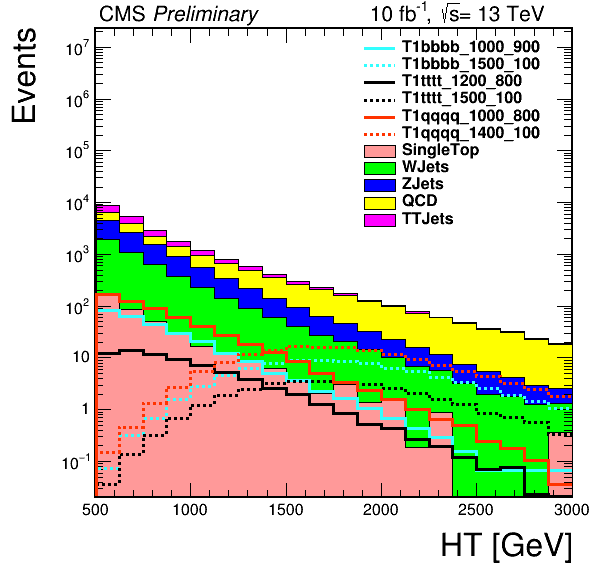
\includegraphics[width=0.35\textwidth]{/home/bibhu/Desktop/PhDThesis/PhDThesis/chapter6/HT_distribution.png}
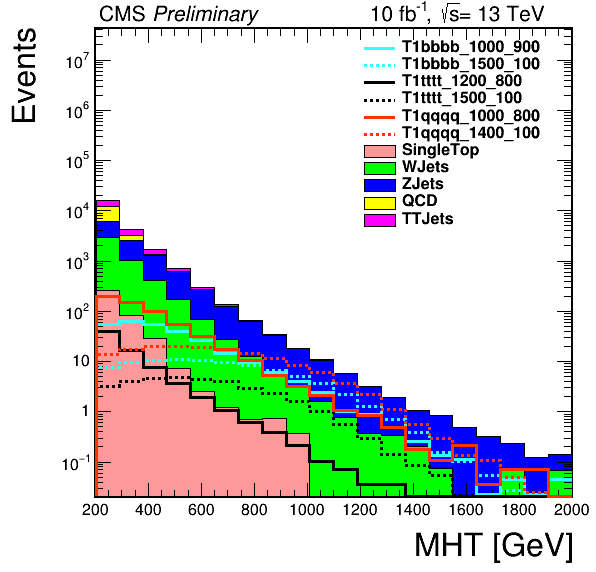
\includegraphics[width=0.35\textwidth]{/home/bibhu/Desktop/PhDThesis/PhDThesis/chapter6/MHT_distribution.png}
\caption{\label{fig:SigvsBkgSearchVariables1Thesis} Signal vs. stacked backgrounds in $\rm H_{T}$(HT, left) and $\rm H_{T}^{miss}$(MHT, right)}
\end{center}
\end{figure}

\begin{figure}[h]
\begin{center}
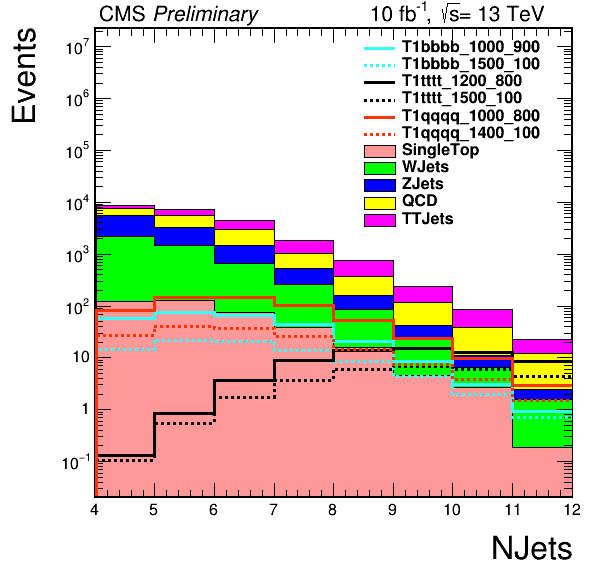
\includegraphics[width=0.35\textwidth]{/home/bibhu/Desktop/PhDThesis/PhDThesis/chapter6/NJets_distribution.png}
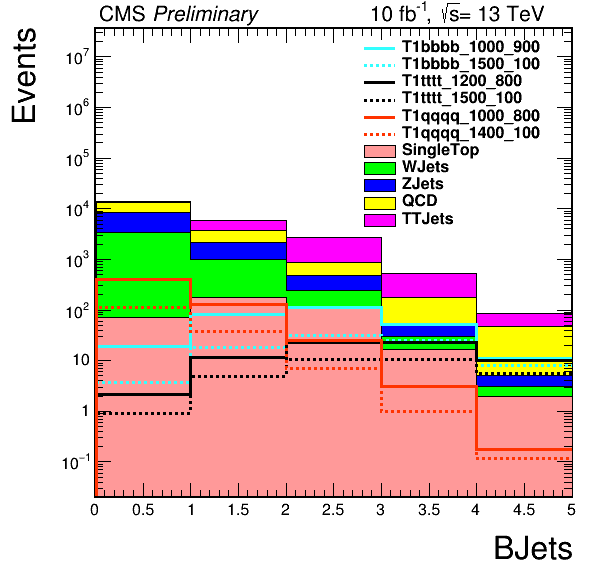
\includegraphics[width=0.35\textwidth]{/home/bibhu/Desktop/PhDThesis/PhDThesis/chapter6/BJets_distribution.png}
\caption{\label{fig:SigvsBkgSearchVariables2Thesis} Signal vs. stacked backgrounds in $\rm N_{jet}$(NJets, left) and $\rm N_{b-jet}$(BJet, right)}
\end{center}
\end{figure}


\end{itemize}

  {\bf Search Binning}


On top of the baseline we split the available phase-space into 72 exclusive intervals to enhance the sensitivity. The search variables and corresponding binning are as follows:
\begin{itemize}
\item $\rm N_{jet}$: 4$-$6, 7$-$8, $\geq 9$;
\item $\rm N_{b-jet}$: 0, 1, 2, $\geq 3$;
\item $\rm H_{T}$: 500$-$800, 800$-$1200, $\geq 1200$ GeV;
\item $\rm H_{T}^{miss}$: 200$-$500, 500$-$750, $\geq 750$ GeV.
\end{itemize}
The analysis is restricted to $\rm N_{jet}\geq 4$ because of our focus
on gluino pair production. The $\rm H_{T}>500 GeV$ and $\rm H_{T}^{miss}>200 GeV$ requirements
are dictated by the trigger conditions. The binning is rectangular as above, except for the 12 bins with $\rm H_{T} < 800 GeV$ 
and $\rm H_{T}^{miss} > 750 GeV$ are removed since $\rm H_{T}^{miss}$ cannot exceed (or be on the order of) $\rm H_{T}$
in a physical event. Additionally, for $\rm 500 <  H_{T}^{miss} < 750 GeV$, a single range with $\rm 500 <  H_{T}\ < 1200 GeV$ is used, and
for $\rm H_{T}^{miss} > 750 GeV$, a single range with $\rm H_{T}\ > 800 GeV$ is used,
because of the lower number of events expected at large $\rm H_{T}^{miss}$. The merging of these bins further
reduces the bin count by 24, to a total of 72 bins. The six bins in the $\rm H_{T}$\ and $\rm H_{T}^{miss}$ plane are
shown visually in Fig.~\ref{fig:HT-MHT}.


\begin{figure}[h]
\begin{center}
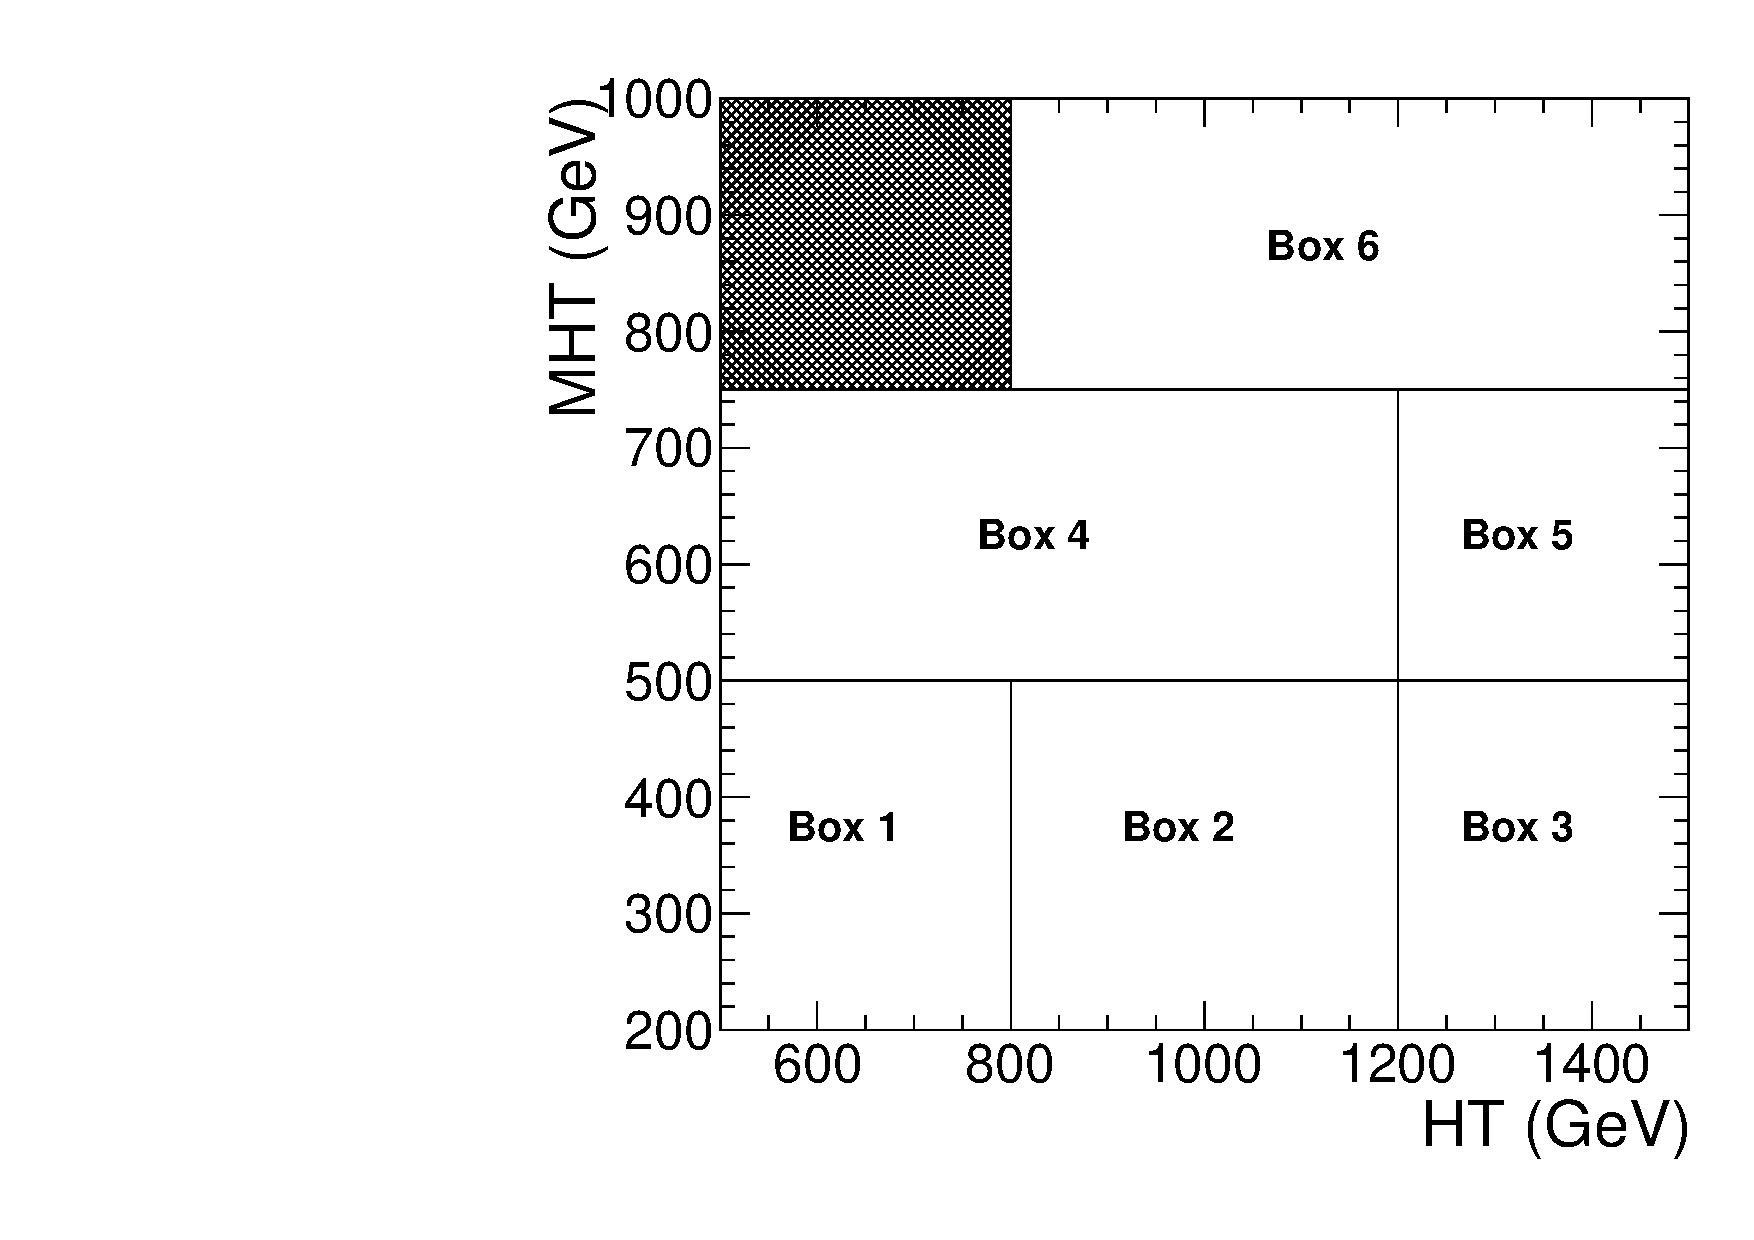
\includegraphics[width=0.35\textwidth]{/home/bibhu/Desktop/PhDThesis/PhDThesis/chapter6/MHT-HT-plane.pdf}

\caption{\label{fig:HT-MHT} Search binning in the 2D phase-space of $\rm H_{T}$ and $\rm H_{T}^{miss}$.}
\end{center}
\end{figure}






\subsection{Backgrounds}


All the SM backgrounds are categorized into four different groups. These are a)Z to invisible, b)Lostlepton, c)Hadronic Tau, d)QCD. Z($\rightarrow \nu\bar{\nu}$)+jets is an irreducible background having exactly the same final state as the signal. The lost lepton background arises when a top or W decays leptonically and the lepton goes unidentified, or non-isolated or out of accepance. In case the W decays to taus with taus subsequently decaying to hadrons, it becomes hadronic tau background. QCD processes have fake MET due to jet energy mismeasurement, so they enter the signal region. All the backgrounds mentioned here are determined using data driven techniques because the MC samples usually do not have accurate simulations for  the higher order processes. Below we will discuss extensively the estimation of Z to invisible background in which we have taken a key role.  

\subsubsection{$Z(\rightarrow \nu \bar{\nu})+jets$ background estimation}

This is the most important backgrounds being an ireducible one. We are talking about events with a Z boson produced in association with jets when the   former decays to two neutrinos. The most straightforward way to measure this background is
to exploit the decays $\rm Z(\ell^{+} \ell^{-})$+jets in which the Z boson can be
reconstructed from an observed pair of muons or electrons.  The
efficiency-corrected yields from these decays can be translated
directly into the $\rm Z(\nu \bar{\nu})$+jets background yield by the known branching
ratios.  The limitation of this approach stems from the rather small
branching ratio between the charged and neutral leptons, so that the
transfer factor from the control sample measurement to the predicted
background is larger than one ;ignoring efficiencies, the
branching ratio itself is approximately 3 when both muon and electron
pairs are used. 

An alternative approach is to exploit the similarity to Z boson
radiation of the more copious radiation of photons.  Here the
challenge is to obtain validation in data of the MC predictions
connecting the two processes.

Our baseline strategy is to use the $\rm \gamma$+jets  sample to determine the
yields in the 18 bins corresponding to $\rm N_{b-jet}$=0.  These are
then compared with the $\rm Z(\ell^{+} \ell^{-})$+jets yields in the low-$\rm N_{jet}$
bins to establish the systematic uncertainty of the physics modeling of
$\rm \gamma$+jets, and the normalization corrected if necessary.  
The extrapolation to bins with $\rm N_{b-jet} >$0 is performed to
the extent possible with the $\rm Z(\ell^{+} \ell^{-})$+jets data sample, supplemented with MC
information where necessary. We use simulation to correct for the
resulting distribution to the higher $\rm N_{jet}$ bins. The master formula that gives the prediction in the 0 b-tagged bins is


%\begin{equation} 

$\bf  N_{Z(\nu\nu)+jets}^{prediction} = \frac{R^{obs}_{Z\rightarrow\ell^{+}\ell^{-}/\gamma}}{R^{MC}_{Z\rightarrow\ell^{+}\ell^{-}/\gamma}} . \frac{N_{Z\rightarrow \nu\bar{\nu}}^{MC}}{N_{\gamma}^{MC}} . (\beta^{EB}_{purity}.N^{data,EB}_{\gamma}+ \beta^{EE}_{purity}.N^{data,EE}_{\gamma}). \frac{1}{C_{data/MC}}$

%\vspace{5cm}

%$\bf \LARGE N_{Z(\nu\nu)+jets}^{prediction} = \rho . \frac{\sigma_{Z\rightarrow\nu\bar{\nu}}^{MC}}{\sigma_{\gamma}^{MC}} . \beta^{\gamma}_{purity} . N^{data}_{\gamma} . \frac{1}{C_{data/MC}}$

%\end{equation}

where 

\begin{itemize}

\item $\bf \rm N_{Z(\nu\nu)+\rm jets}^{prediction}$ is the number of predicted $Z(\nu\nu)+jets$ events in the search bins.


\item $\bf \rm N^{data,EB}_{\gamma}$ and $\rm N^{data,EB}_{\gamma}$ are the number of single photon events observed in data in barrel and endcap respectively.


\item  $\bf \rm \beta^{EB}_{purity}$ and $\beta^{\rm EE}_{\rm purity}$ are the photon purity in the barrel and endcap, respectively. Single photon events get contaminated from $\pi^{0} \rightarrow \gamma\gamma$ processes. We measure the purity also using data driven techniques. This will be discussed in the following sections. 



\item $\bf \rm R^{MC}_{Z\rightarrow\ell^{+}\ell^{-}/\gamma}$ is the ratio of production rates at the reconstruction level. This is calculated using MC events. But as we do not trust montecarlo fully, we derive a correction to this ratio by calculating a double ratio. Double ratio is defined as the ratio of  $\rm Z\rightarrow\ell^{+}\ell^{-}$ events to $\rm \gamma + jets$ events calculated in data and montecarlo respectively.


\end{itemize}


{\bf Photon Reconstruction}

For the photon$+$jets control sample, we require at least one well identified and isolated photon candidate having a minimum $\rm p_{T}$ of 100 GeV of transverse momentum and pseudorapidity $|\eta|<2.5$, excluding the barrel-endcap transition, $1.4442<|\eta|<1.566$.  Identification and isolation requirements, intended to reject electrons and pions misreconstructed as photons, are adopted from the Egamma POG's recommendations for 8 TeV and 13 TeV analysises.  The identification criteria, which include requirements for low hadronic activity ($H/E$), a shower shape ($\sigma_{i\eta i\eta}$) consistent with a photon, and an associated pixel seed veto, are shown in Table~\ref{tab:IDISOcuts} for events with a photon in the barrel or endcap.

The isolation requirements restrict the energy sum from PF candidates within a cone of $\Delta R<0.3$ around the momentum vector of the photon candidate.  Specifically, we require that the energy from charged hadrons (Iso$_{\rm pfCh.}$), neutral hadrons (Iso$_{\rm pfNu.}$), and electromagnetic particles Iso$_{\rm pfGa.}$ not to exceed the $p_{\rm T}$-dependent thresholds listed in Table~\ref{tab:IDISOcuts}.  The isolation energy from each of the three particle species is corrected for pileup with the per-event average pileup energy density ($\rho$) and per-photon $\eta$-dependent effective area listed in Table~\ref{tab:effarea}.  


\begin{table}[h]
\begin{center}
\caption{Identification and isolation requirements for photons in the barrel and endcap. EA stands for effective area.}
\begin{tabular}{|l|c|c|}
\hline
Variable & Barrel & Endcap \\ 
\hline
Pixel Seed Veto & Yes & Yes \\
H/E & $<$0.05 & $<$0.05 \\
$\sigma_{i\eta i\eta}$ & $<$0.011 & $<$0.031 \\
\hline
max(Iso$_{\rm pfCh.}$ - EA$\cdot\rho$ , 0 ) & $<$0.7 & $<$0.5 \\
max(Iso$_{\rm pfNu.}$ - EA$\cdot\rho$ , 0 ) & $<$0.4 + 0.04$\times p_{\rm T}$ & $<$1.5+0.04$\times p_{\rm T}$ \\
max(Iso$_{\rm pfGa.}$ - EA$\cdot\rho$ , 0 ) & $<$0.5 + 0.005$\times p_{\rm T}$ & $<$1.0+0.005$\times p_{\rm T}$ \\
\hline
\end{tabular}
\label{tab:IDISOcuts} 
\end{center}
\end{table}

\begin{table}[h]
\begin{center}
\caption{Effective areas used in pileup correction as a function of photon pseudorapidity. Three columns shows different effective areas used for calculating Iso$_{\rm pfCh.}$, Iso$_{\rm pfNu.}$ and Iso$_{\rm pfGa.}$, respectively in various $\eta$ bins. }
\begin{tabular}{|c|c|c|c|}
\hline 
$|\eta|$  & EA(pfCh.) & EA(pfNu.) & EA(pfGa.) \\ \hline 
0.0 - 1.0 & 0.012 & 0.030 & 0.148 \\ 
1.0 - 1.479 & 0.010 & 0.057 & 0.130 \\
1.479 - 2.0 & 0.014 & 0.039 & 0.112 \\
2.0 - 2.2 & 0.012 & 0.015 & 0.216 \\
2.2 - 2.3 & 0.016 & 0.024 & 0.262 \\
2.3 - 2.4 & 0.020 & 0.039 & 0.260 \\
$>$ 2.4 & 0.012 & 0.072 & 0.266 \\
\hline 
\end{tabular}
\label{tab:effarea}
\end{center}
\end{table}


{$\rm N_{\gamma}^{\rm obs}$ and photon categories: }


The photons in the control sample come from three sources: direct prompt photons, fragmentation 
prompt photons, and non-prompt photons.  Prompt photons are radiated from a quark while non-prompt photons come 
from the decay of a meson. Direct(fragmentation) prompt photons are radiated with relatively (small) large transverse momentum 
relative to the quark; fragmentation prompt photons are radiated with low transverse momentum relative 
to the quark.  

Direct prompt photons, which make up about $85\%$ of the control sample, are the most useful in predicting 
the $Z\to\nu\nu$ background because their production processes most neatly map onto the set of $Z$ boson 
production processes. As processes leading to non-prompt photons have no corresponding process for 
 those leading to $Z$ bosons, non-prompt photons do not contribute to the $Z\to\nu\nu$ background estimation 
.  At the most basic level, the correspondence (or lack thereof) between fragmentation photon 
 and $Z$ processes is less straightforward, and the special treatment of this photon category 
is instead motivated by practical considerations %(Sec.~\ref{sec:rzg}).  

In practice, we categorize photons in the simulation as 
\begin{itemize}
\item prompt photons: stable final state photons with its parent either a photon, quark or proton. 
  \begin{itemize}
  \item direct prompt photons: prompt photons with $\Delta R >0.4$ with respect to any quarks or gluons, 
  \item fragmentation prompt photons: all prompt photons that are not direct, and
  \end{itemize}
\item non-prompt photons: all photons that are not prompt.
\end{itemize} 
Any photon in the $\gamma$+jets or QCD samples is either non-prompt, direct prompt, or fragmentation prompt.  Any prompt photon is either direct prompt or fragmentation prompt. 
\begin{figure}[h]
\begin{center}
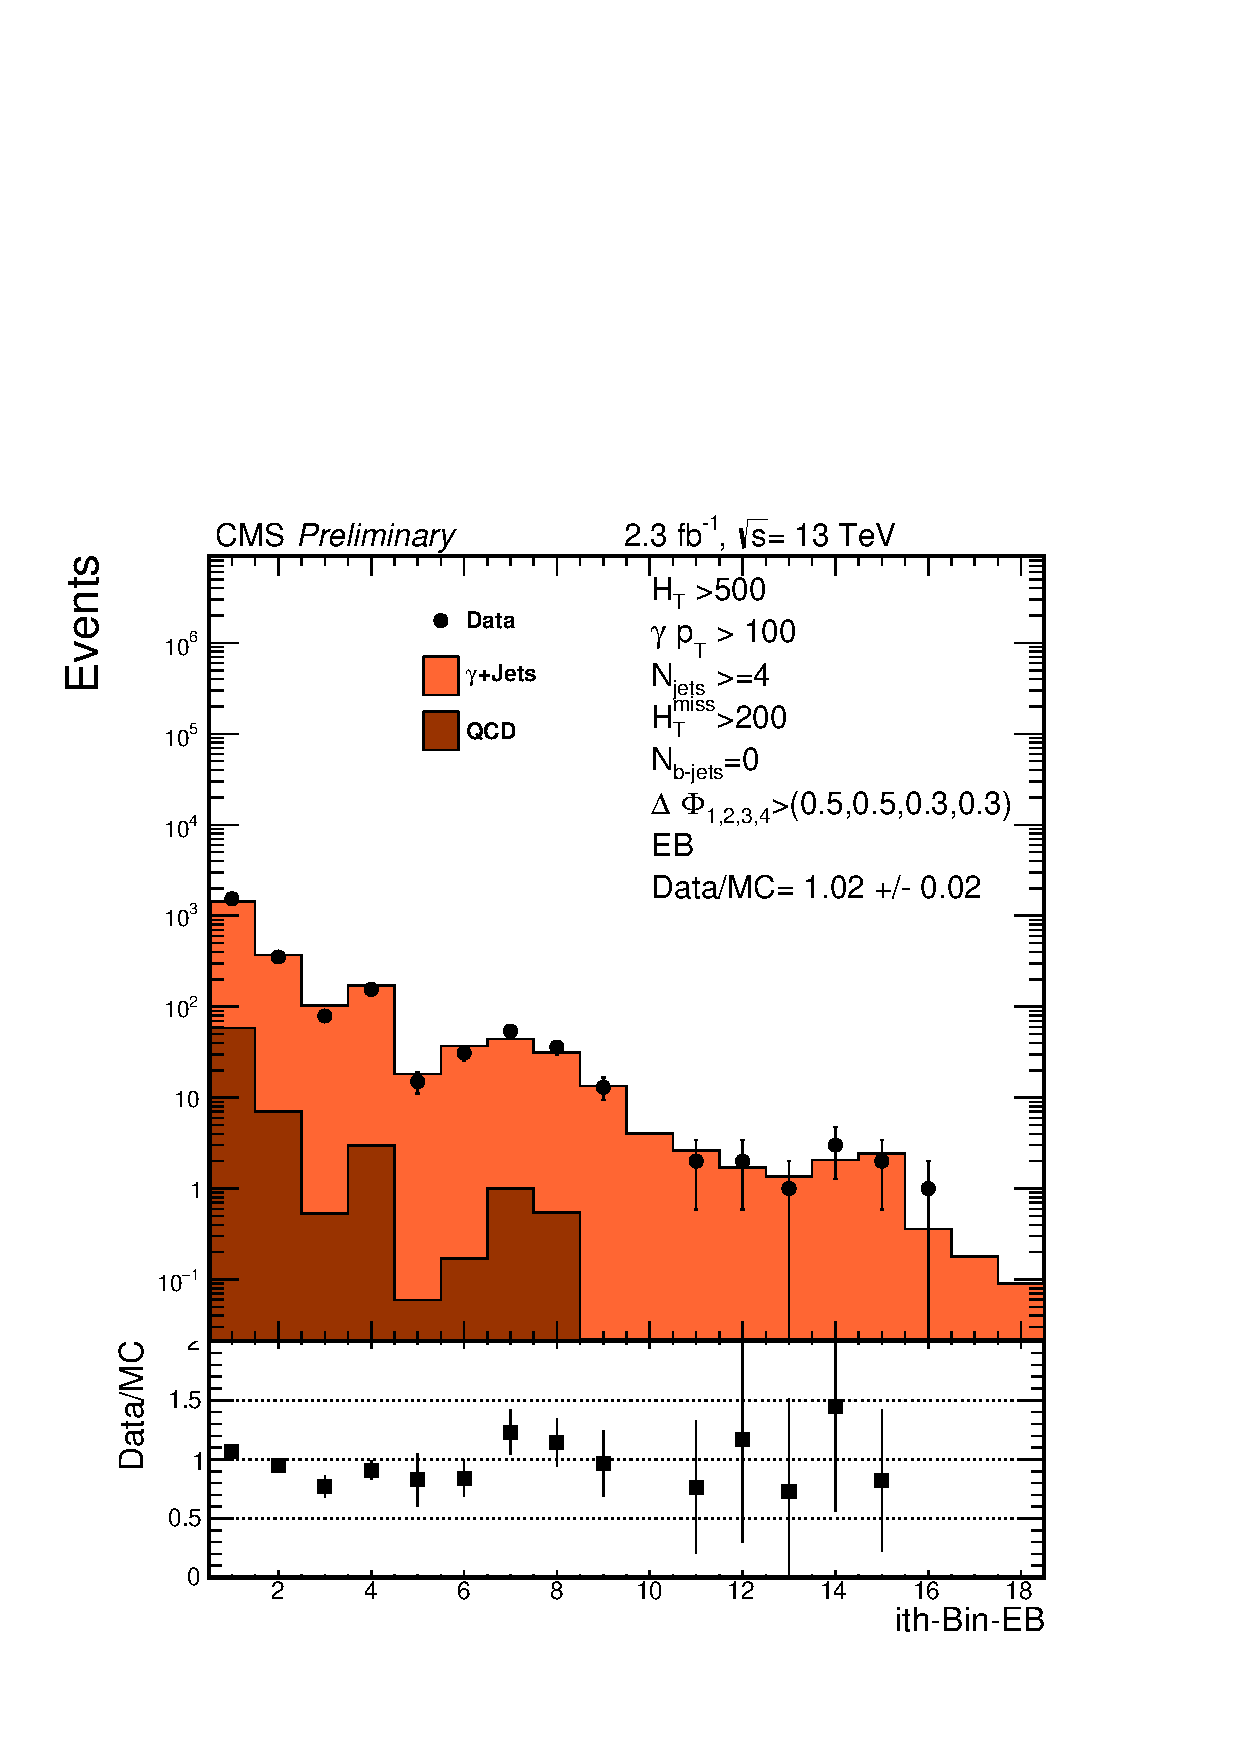
\includegraphics[width=0.48\textwidth]{/home/bibhu/Desktop/PhDThesis/PhDThesis/chapter6/ith-Bin-EB__Data_MC_EB.pdf} % ADDNEWPLOT 
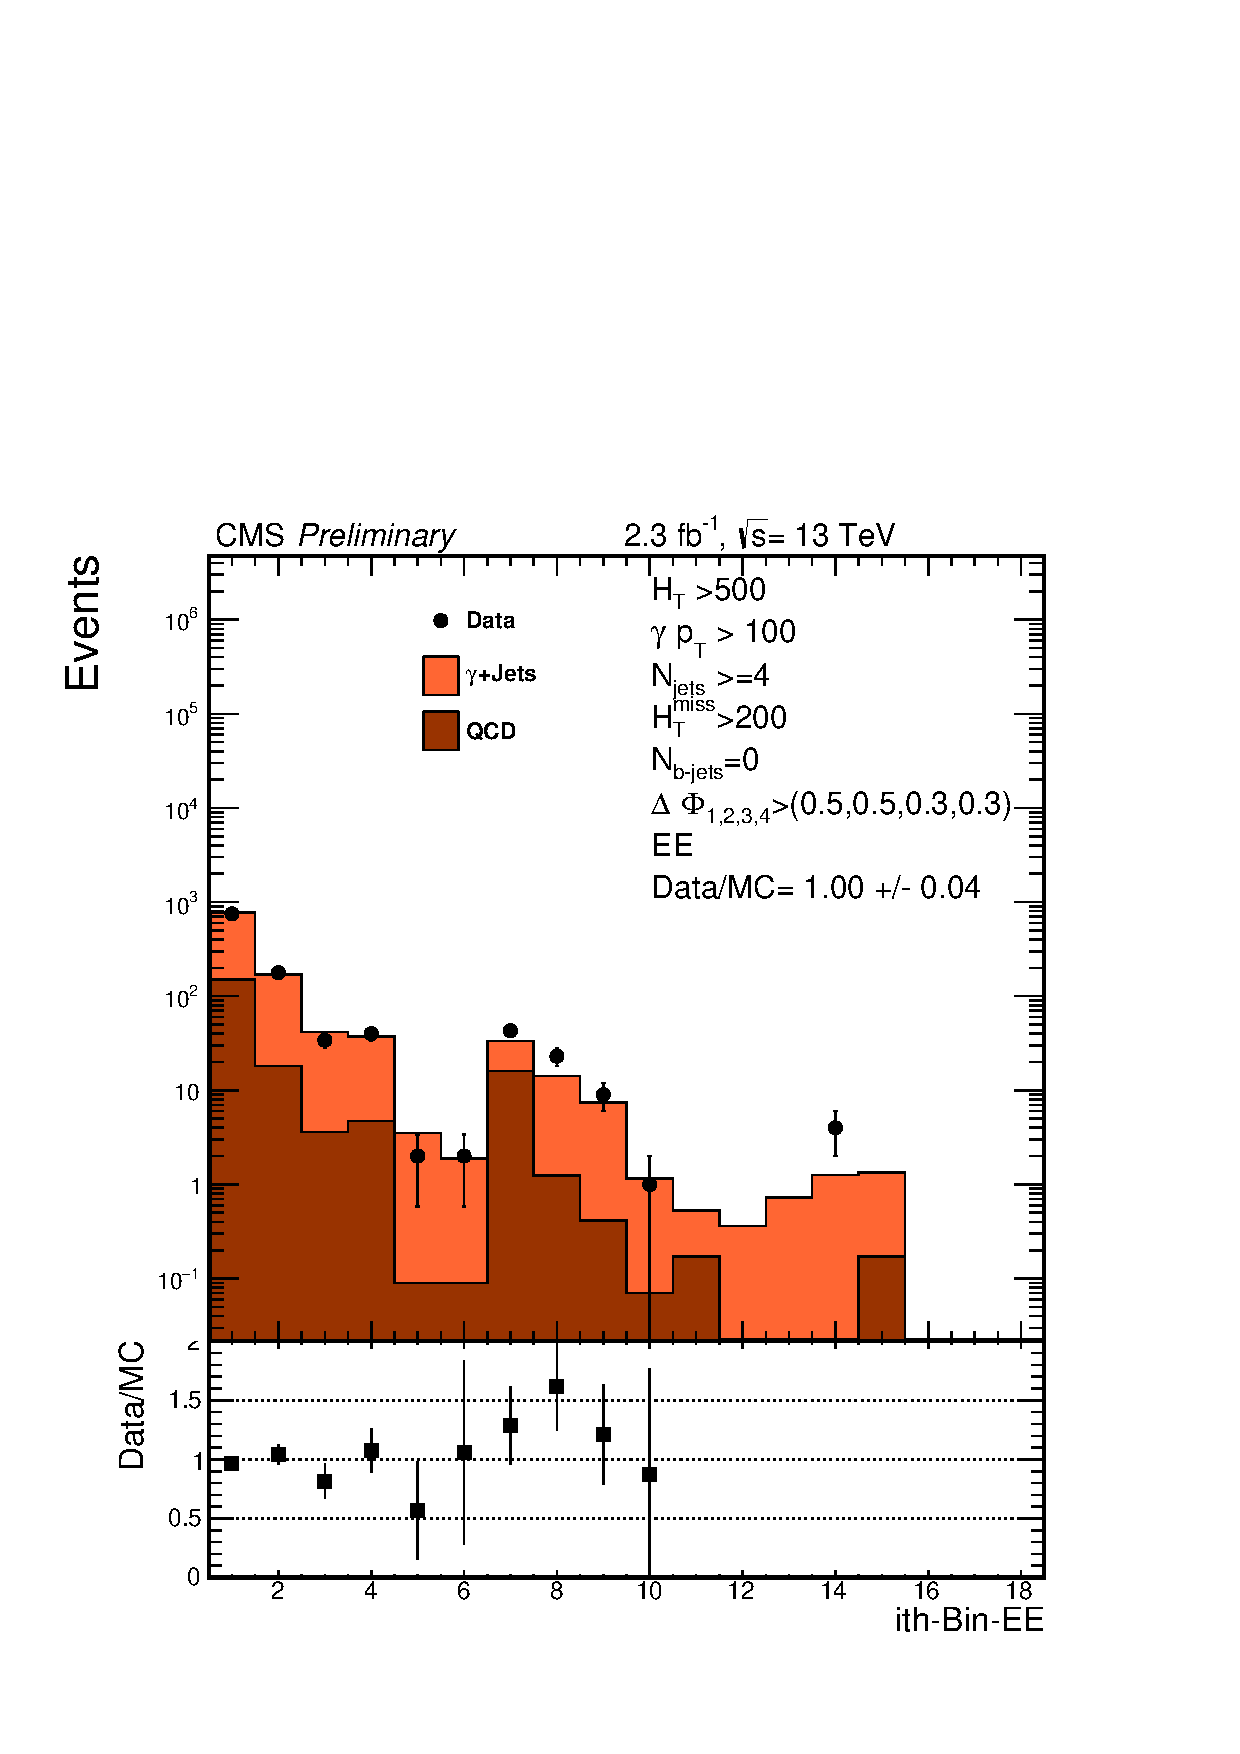
\includegraphics[width=0.48\textwidth]{/home/bibhu/Desktop/PhDThesis/PhDThesis/chapter6/ith-Bin-EE__Data_MC_EE.pdf} % ADDNEWPLOT 
\caption{Numbers of observed events in the photon control samples in barrel (left) and endcap (right) compared to simulation.}
\label{fig:nobs}
\end{center}
\end{figure}

The numbers of observed photons in ECAL barrel (EB) and endcap (EE) are shown in Fig.~\ref{fig:nobs}.
There is no systematic uncertainty on $N_{\gamma}^{\rm obs}$ because it is a simple observation.  The 
statistical uncertainty related to this observation is included in the statistical analysis when a 
Poisson PDF is assigned to this variable.

{\bf Purity:}


%\label{sec:purity} 
The purity $\beta$ is defined as the fraction of all photons (prompt+non-prompt) that are prompt: 
$\beta = N_{\rm prompt} / (N_{\rm prompt}+N_{\rm non-prompt})$.  In practice, we allow the purity 
to depend on photon $\rm p_{T}$, which is essentially equivalent to event $\rm H_{T}^{miss}$.  We also explore 
differences in purity for ECAL barrel and endcap separately.

%\begin{align}
%N_{Z\to\nu\nu}^{\rm pred} &= {\cal R}_{Z(\nu\bar{\nu})/\gamma} \cdot {\cal F}_{\rm dir} \cdot ( \beta_{\rm low \MHT} N_{\gamma, \rm EB}^{\rm obs} + \beta_{\rm EE} N_{\gamma, \rm EE}^{\rm obs}).
%\label{eq:gjet2}
%\end{align}

Prompt photons can be distinguished from non-prompt ones by the differences in shape of their 
showers in the ECAL, as described by the well known quantity $\sigma_{i\eta i\eta}$. 
The purity is determined with a two-component determined to the $\sigma_{i\eta i\eta}$ distribution 
in the photon control sample.  The PDF for the prompt component is fit directly in data
using a Gaussian function, which was motivated by the $\gamma$+jets 
{\sc MadGraph} simulation, and the PDF for the non-prompt component comes from the QCD 
{\sc MadGraph} simulation.    The fit result is $(96.3 \pm 0.6)\%$ for $\rm H_{T}^{miss}$ in the range 200-500 GeV 
and $(90 \pm 3)\%$ for $\rm H_{T}^{miss} > 500$ GeV. Results of the EB and EE purity fits are shown in Fig.~\ref{fig:purity}. 

\begin{figure}[h]
\begin{center}
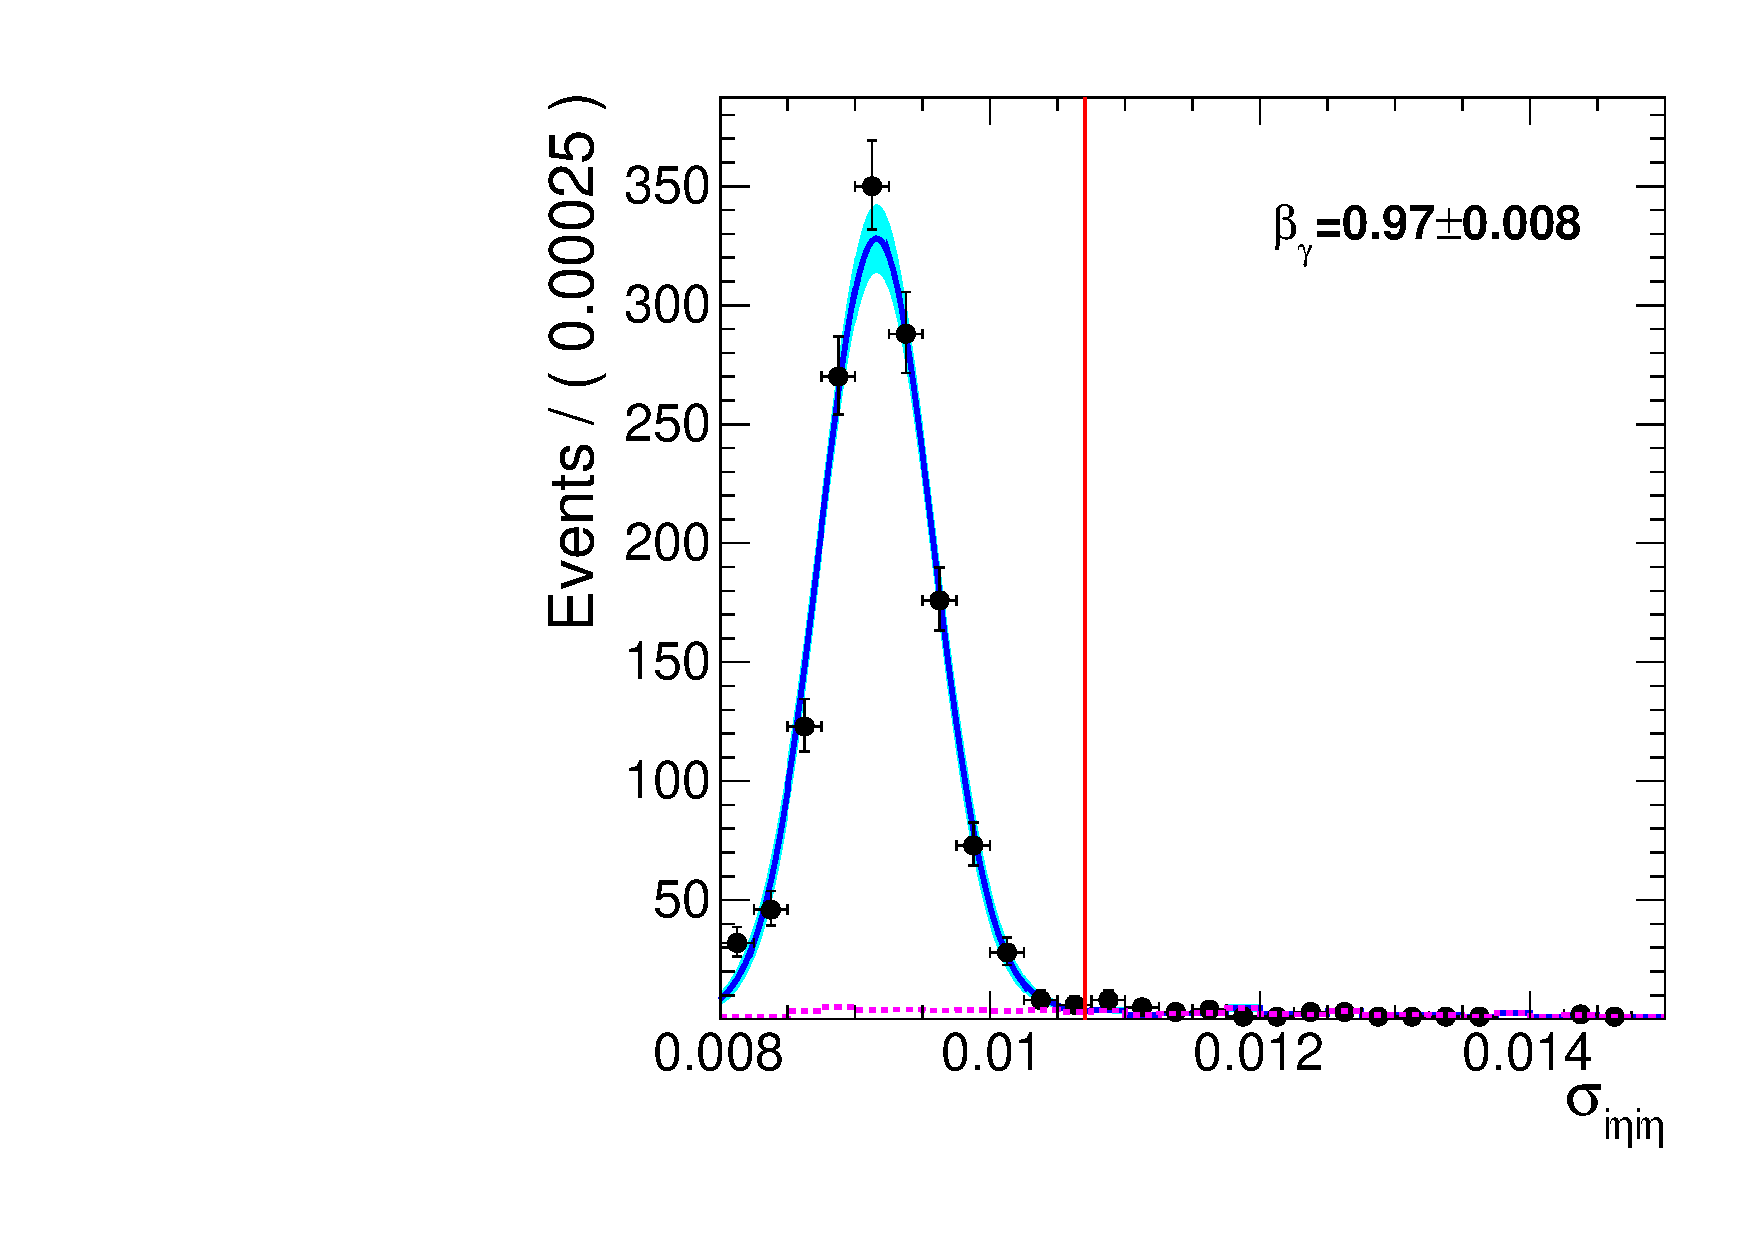
\includegraphics[width=0.32\textwidth]{/home/bibhu/Desktop/PhDThesis/PhDThesis/chapter6/purityFit_MHTlow_barrel2p1.pdf} 
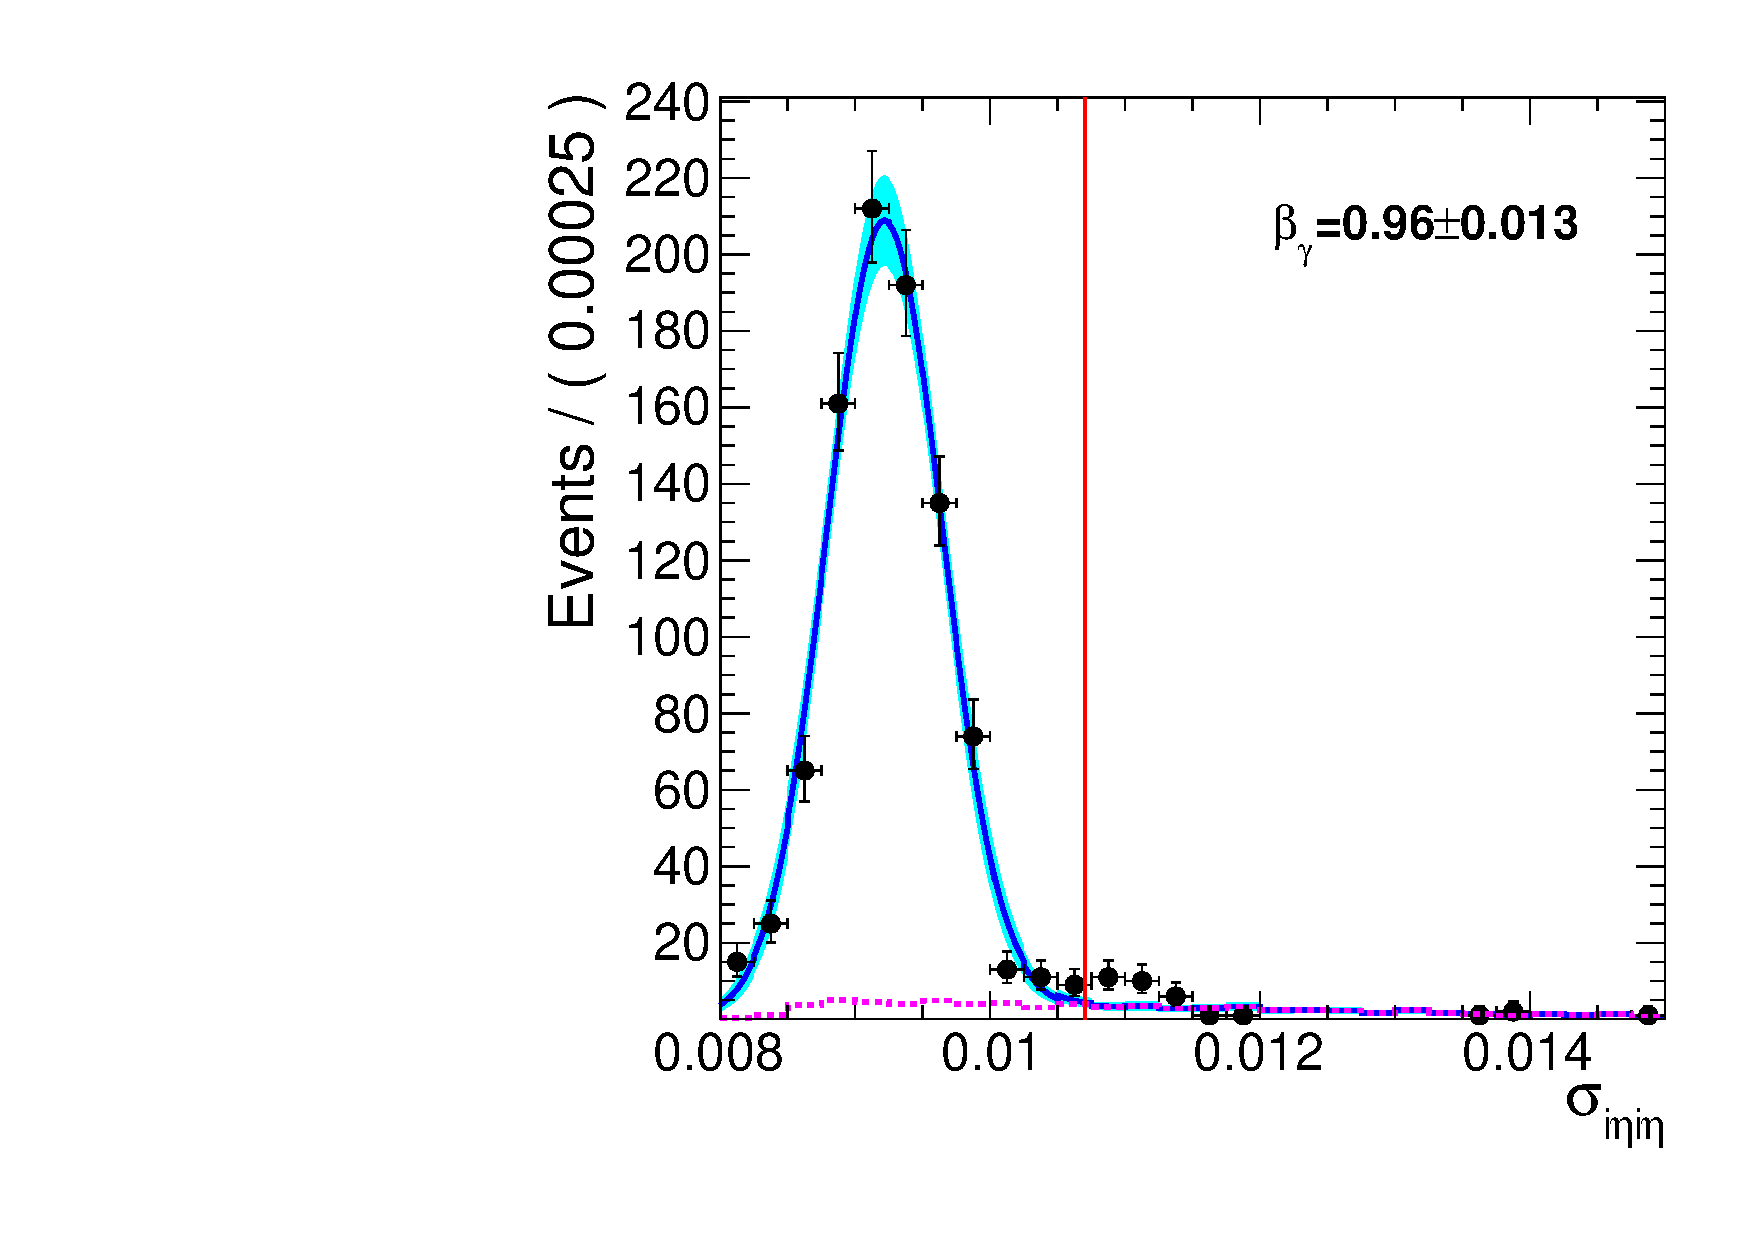
\includegraphics[width=0.32\textwidth]{/home/bibhu/Desktop/PhDThesis/PhDThesis/chapter6/purityFit_MHTmed_barrel2p1.pdf} 
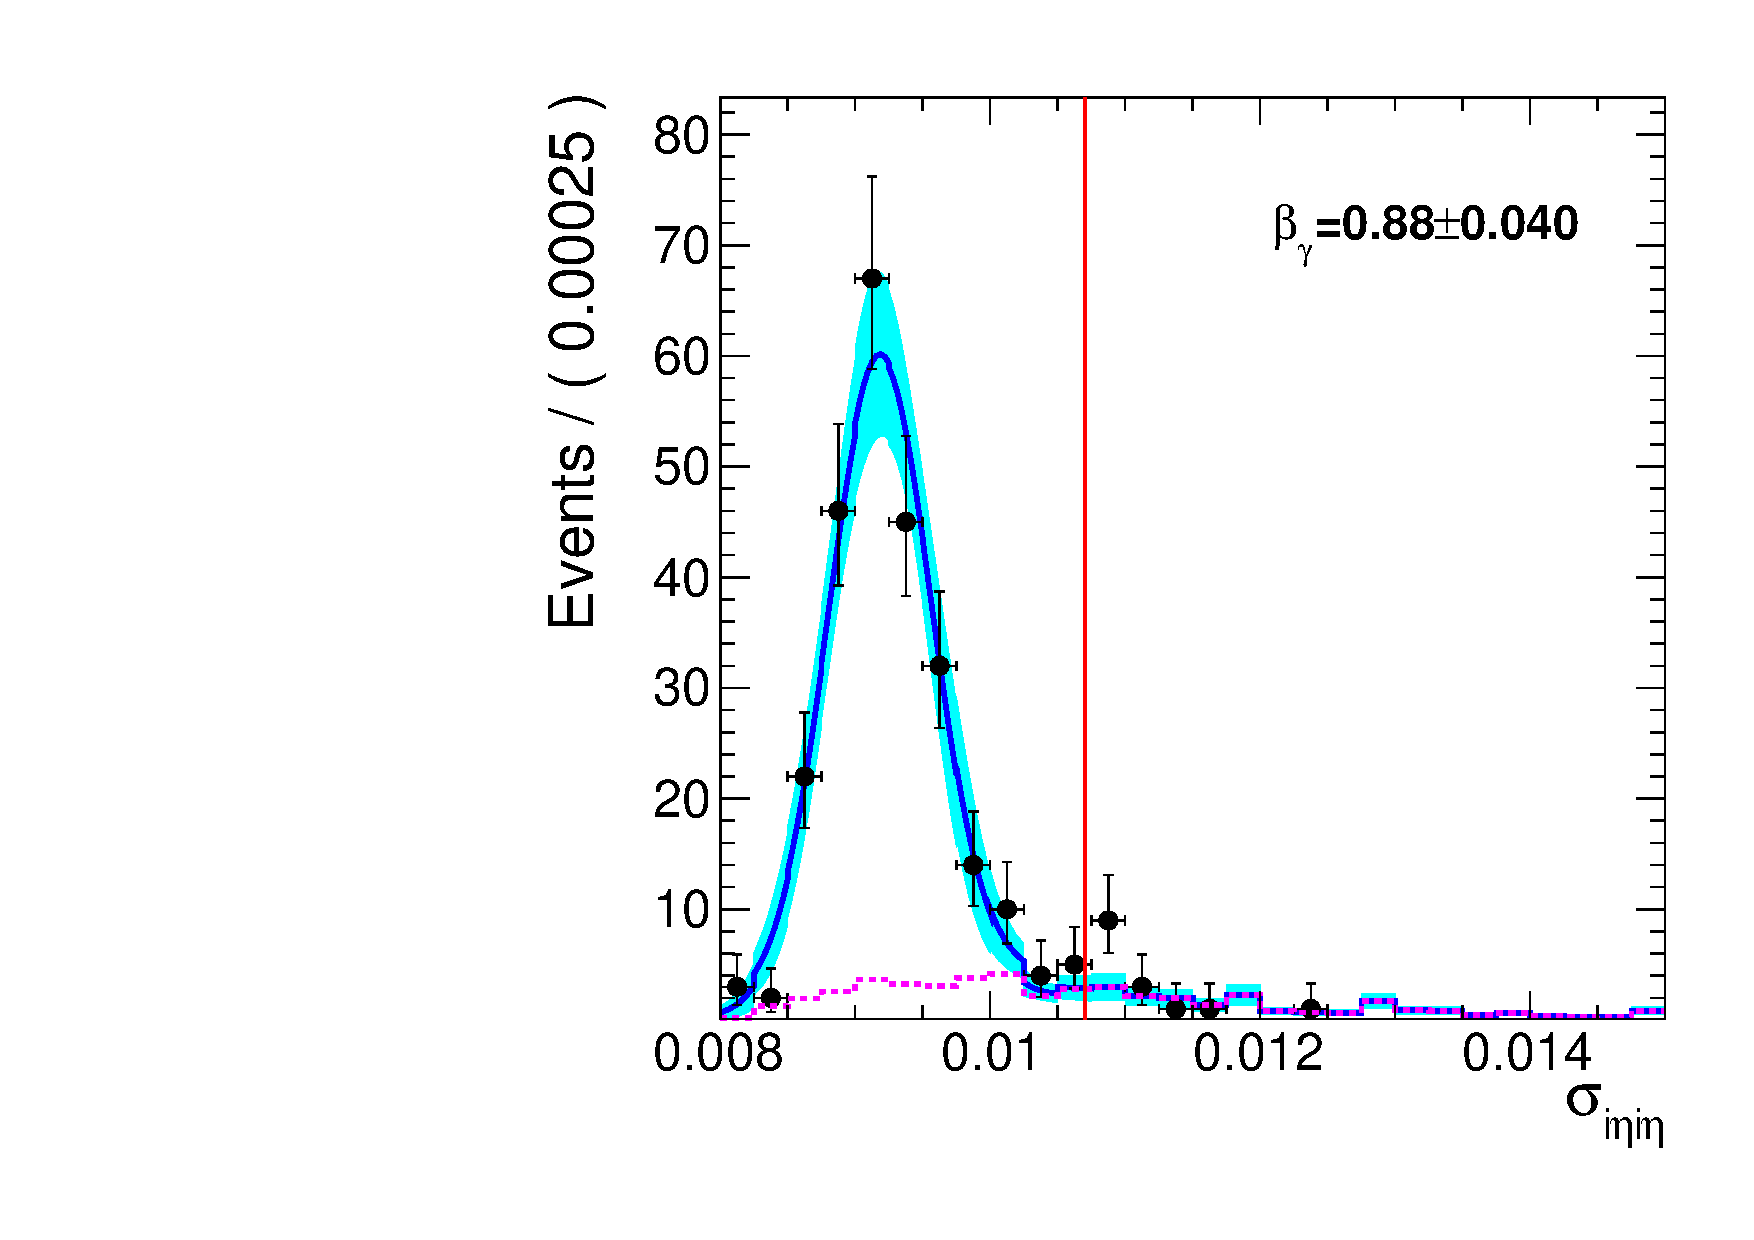
\includegraphics[width=0.32\textwidth]{/home/bibhu/Desktop/PhDThesis/PhDThesis/chapter6/purityFit_MHThigh_barrel2p1.pdf} 
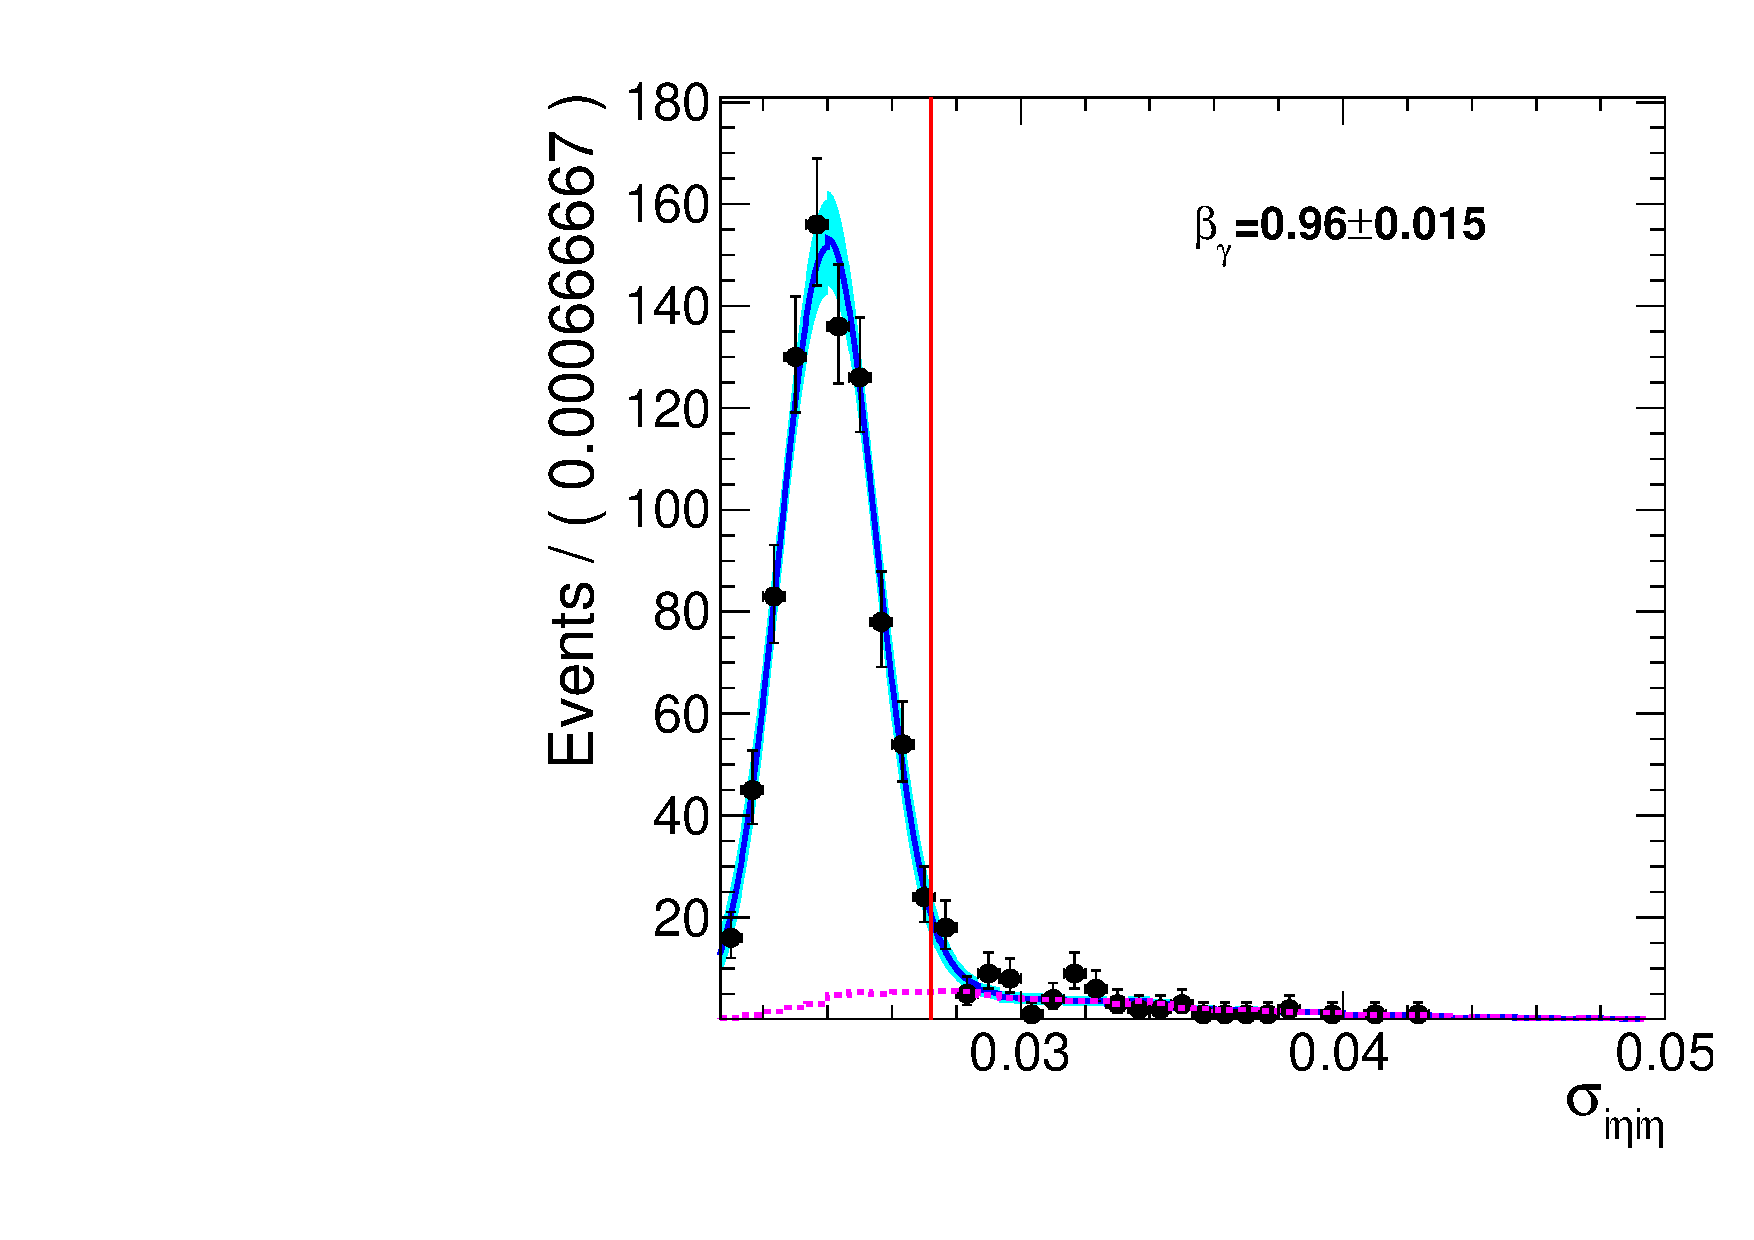
\includegraphics[width=0.32\textwidth]{/home/bibhu/Desktop/PhDThesis/PhDThesis/chapter6/purityFit_MHTlow_endcap2p1.pdf} 
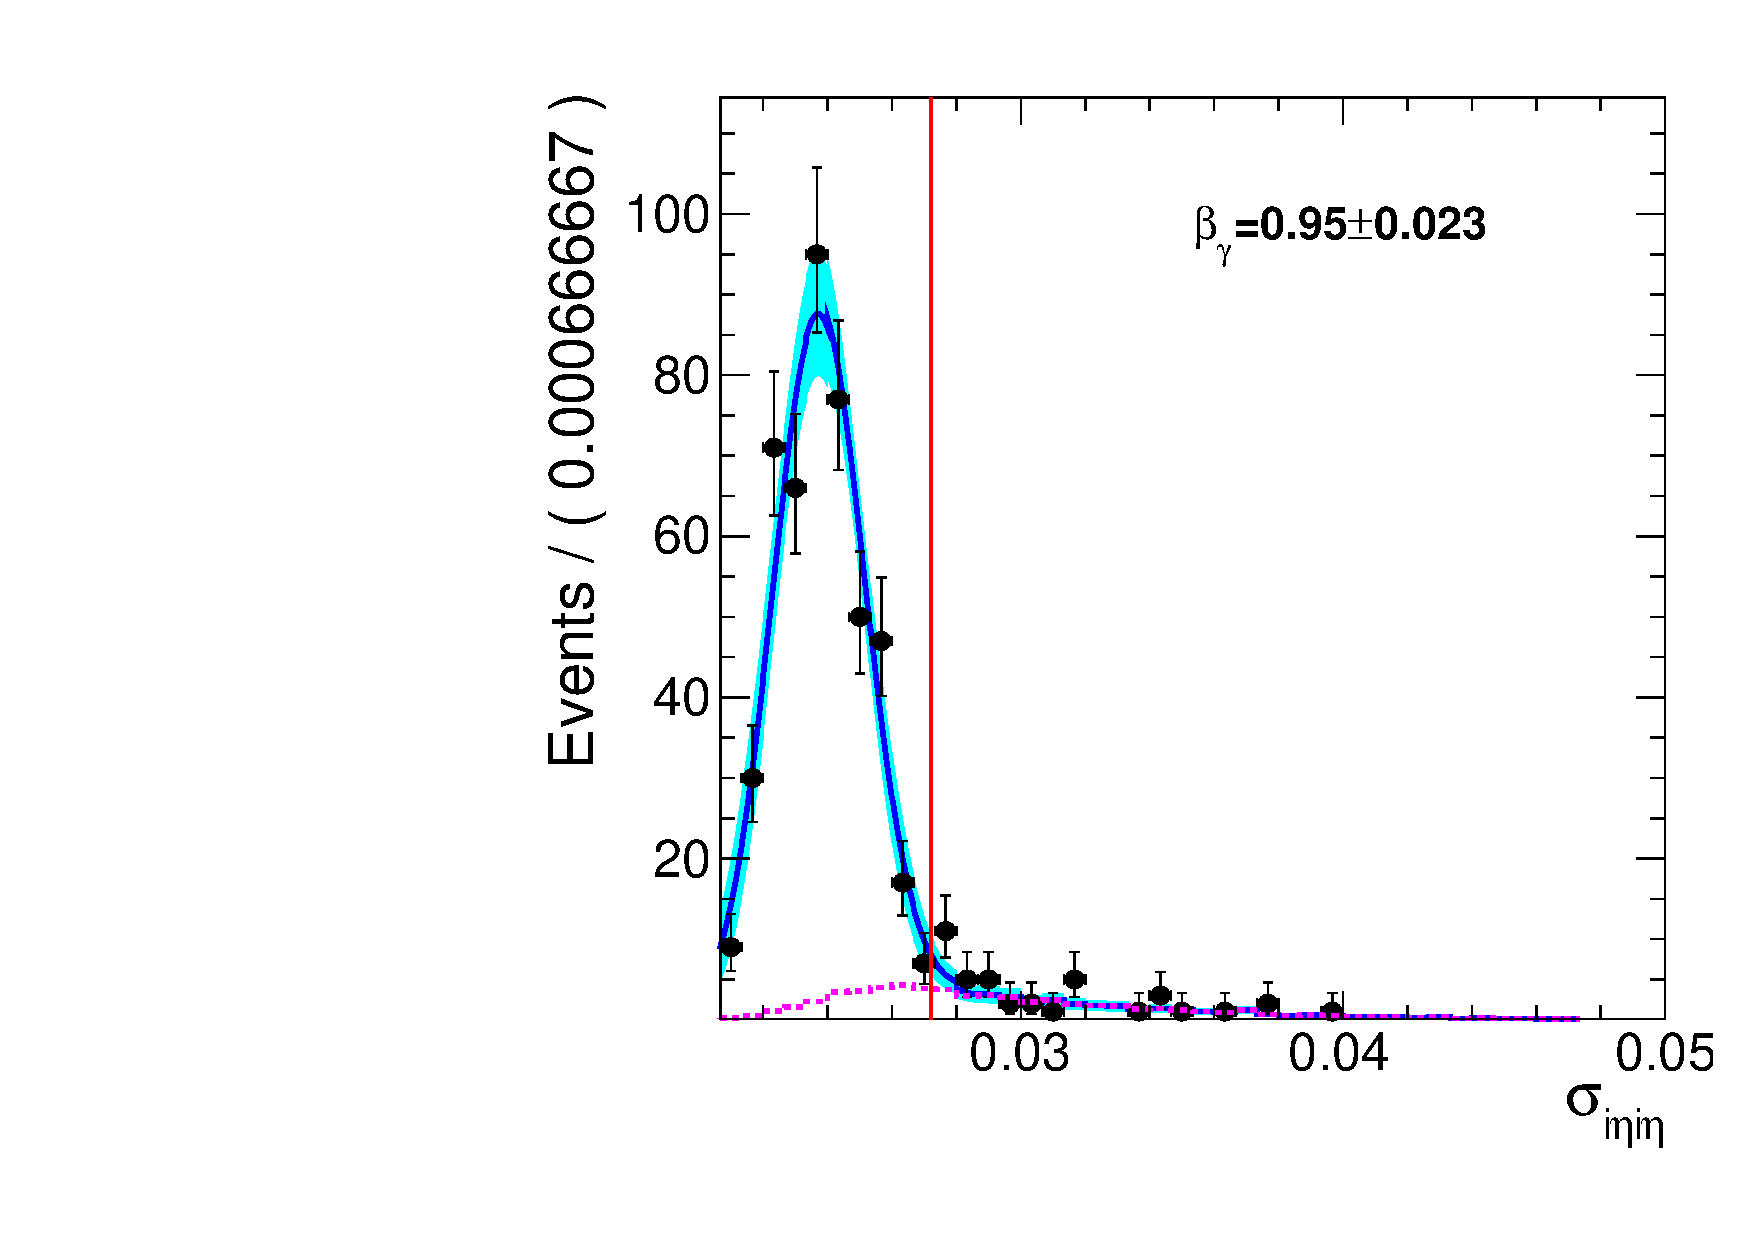
\includegraphics[width=0.32\textwidth]{/home/bibhu/Desktop/PhDThesis/PhDThesis/chapter6/purityFit_MHTmed_endcap2p1.pdf} 
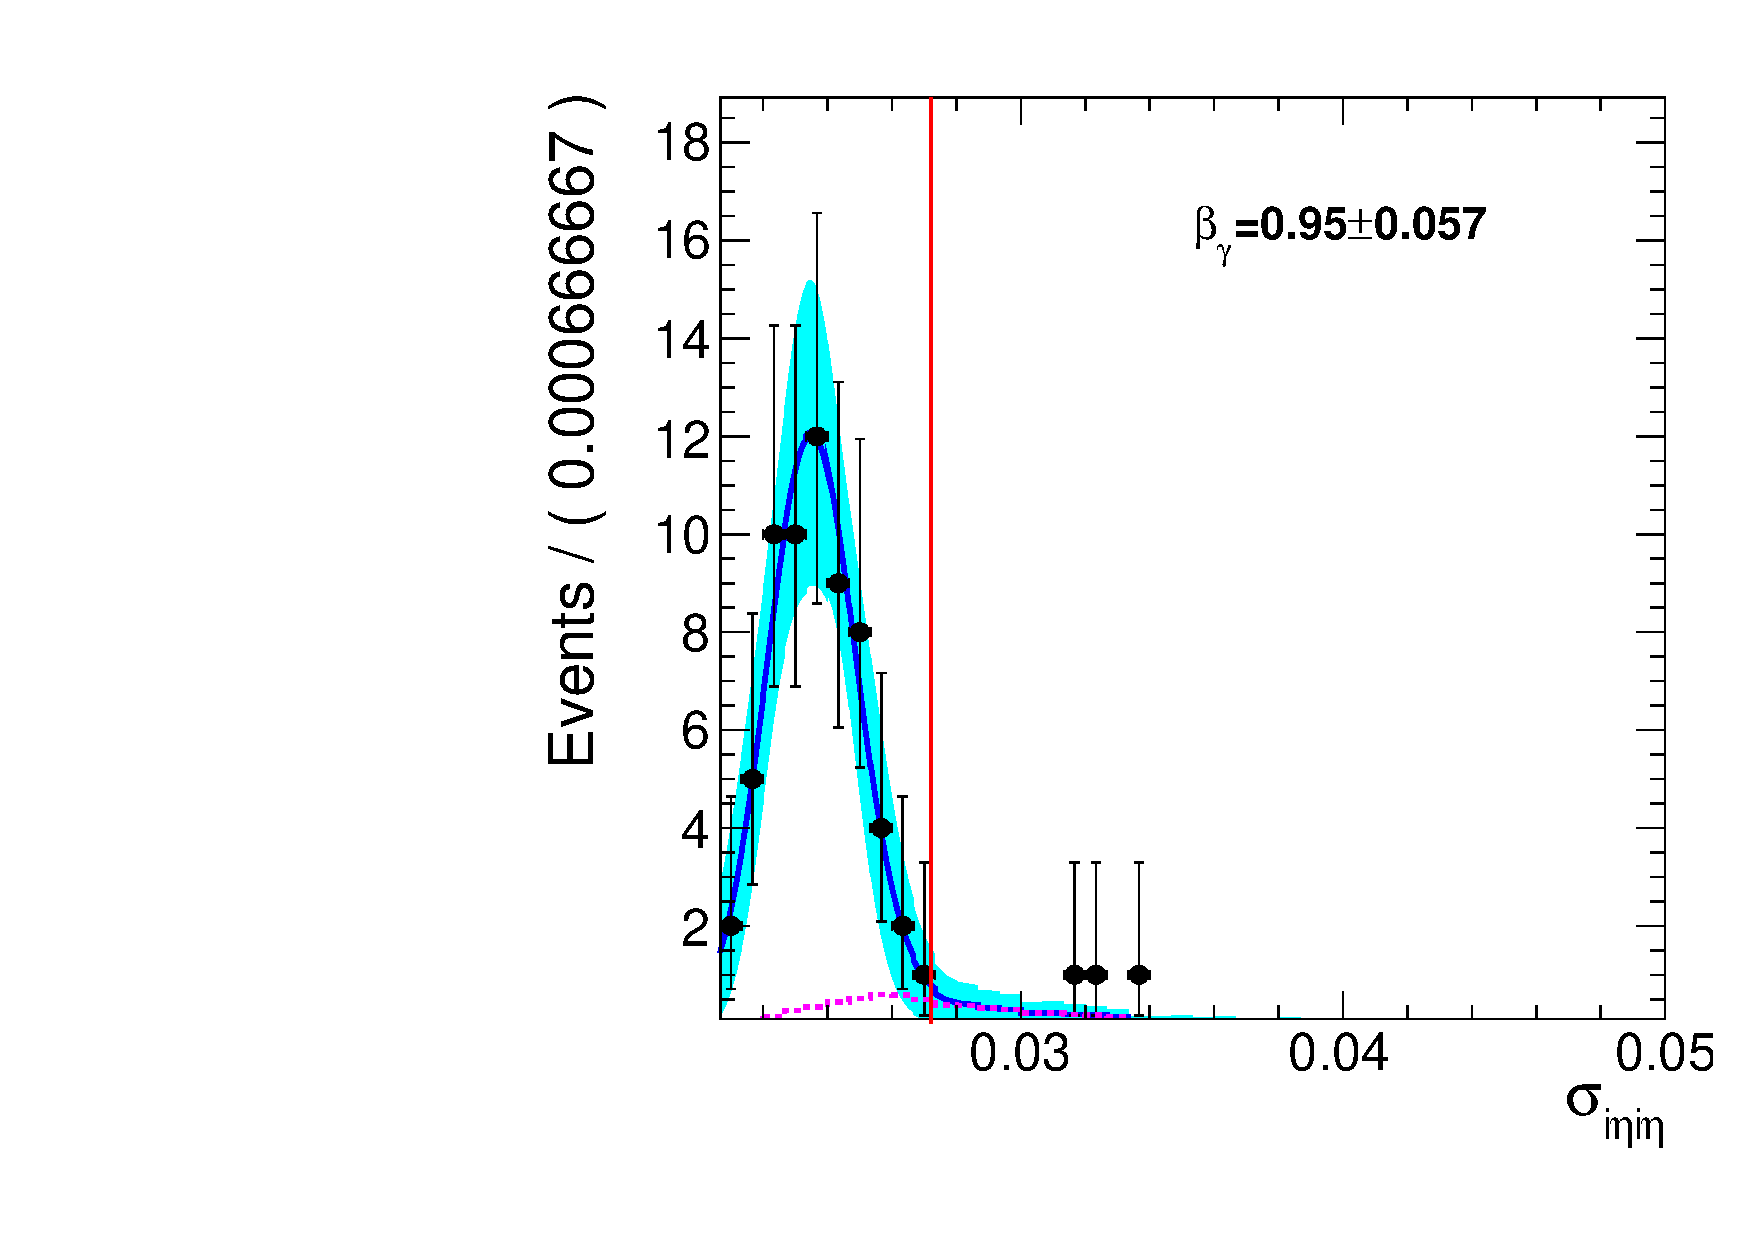
\includegraphics[width=0.32\textwidth]{/home/bibhu/Desktop/PhDThesis/PhDThesis/chapter6/purityFit_MHThigh_endcap2p1.pdf} 
\caption{Fit results for purity determination in EB (top) and EE (bottom) for events with $\rm H_{T}^{miss}$ in the range 200-300, 300-500, and for $\rm H_{T}^{miss} > 500$, 
respectively.  $\beta_\gamma$ is the fitted purity within the corresponding region.  The red vertical line shows the $\sigma_{i\eta i\eta}$ 
requirement for the loose ID working point.  The non-prompt PDF comes from the QCD simulation.}
\label{fig:purity}
\end{center}
\end{figure}

To obtain the systematic uncertainty on purity we perform the purity fits additional times with alternative prompt and 
non-prompt PDFs, and we take the difference in resulting purity as the systematic uncertainty.  The %App.~\ref{app:gammajets}, 
the photon control sample is defined with a requirement on the charge isolation of photon candidates.
For the alternative non-prompt PDF, we obtain a sample of mostly non-prompt photons by inverting 
the charge isolation requirement, and we use the $\sigma_{i\eta i\eta}$ shape from these photons as the PDF.
We also considered using a template derived from $\gamma$+jets simulation as an alternative prompt PDF
%For the alternative prompt PDF, we parameterize the shape with a Guassian distribution and allow the width to vary in the fit.
The variation in purity result for the alternative prompt PDF is negligible.  
The variation in purity result for the alternative non-prompt PDF is about $4\%$.
%Results of these purity fits are shown in Fig.~\ref{fig:purity_syst}. 
We take the quadrature sum of the difference in fit and the statistical uncertainty on the nominal fit as the systematic 
uncertainty on the purity; the systematic uncertainty is uncorrelated across different $\rm H_{T}^{miss}$ bins.



{\bf ${\cal R}_{Z(\nu\bar{\nu})/\gamma}$ and ${\cal F}_{\rm dir}$}
%\label{sec:rzg}

To account for the difference in cross sections and small differences 
in kinematic distributions of Z and $\gamma$ events, we apply a scale 
factor ${\cal R}_{Z(\nu\bar{\nu})/\gamma}$ which is the ratio of the 
number of $Z\to\nu\nu$+jets and $\gamma$+jets events computed with 
LO generator-level simulation ({\sc Madgraph}+{\sc Pythia}) 
in each analysis bin.  The numerator and denominator are both determined 
after full selection at the reconstruction, instead of generation, physics 
objects. Fig.~\ref{fig:rzg} shows ${\cal R}_{Z(\nu\bar{\nu})/\gamma}$ in the 18 0-btagged bins. 


As ${\cal R}_{Z(\nu\bar{\nu})/\gamma}$ is determined at reconstruction level , we correct ${\cal R}_{Z(\nu\bar{\nu})/\gamma}$ for potential data-MC scale factors (SFs)  for efficiency related to photon reconstruction,  identification, isolation, and trigger.  
These SFs have been computed for our selection as functions of photon $E_{\rm T}$, photon 
$\eta$, $\rm N_{jet}$, and $\Delta R(\gamma$,nearest jet$)$.  Preliminary results show that 
the SFs are independent of the analysis variables, so we correct for the efficiency by the 
single value of $0.98\pm0.05$ when computing ${\cal R}_{Z(\nu\bar{\nu})/\gamma}$, and  
vary the SF by a $5\%$ to determine the systematic uncertainty.

Two different kinds of uncertaities are shown in Fig.~\ref{fig:rzg}. The statistical ones from finite MC statistics and the systematic ones are obtained by propagating the ID/Iso SF to  ${\cal R}_{Z(\nu\bar{\nu})/\gamma}$.
  
\begin{figure}[h]
\begin{center}
  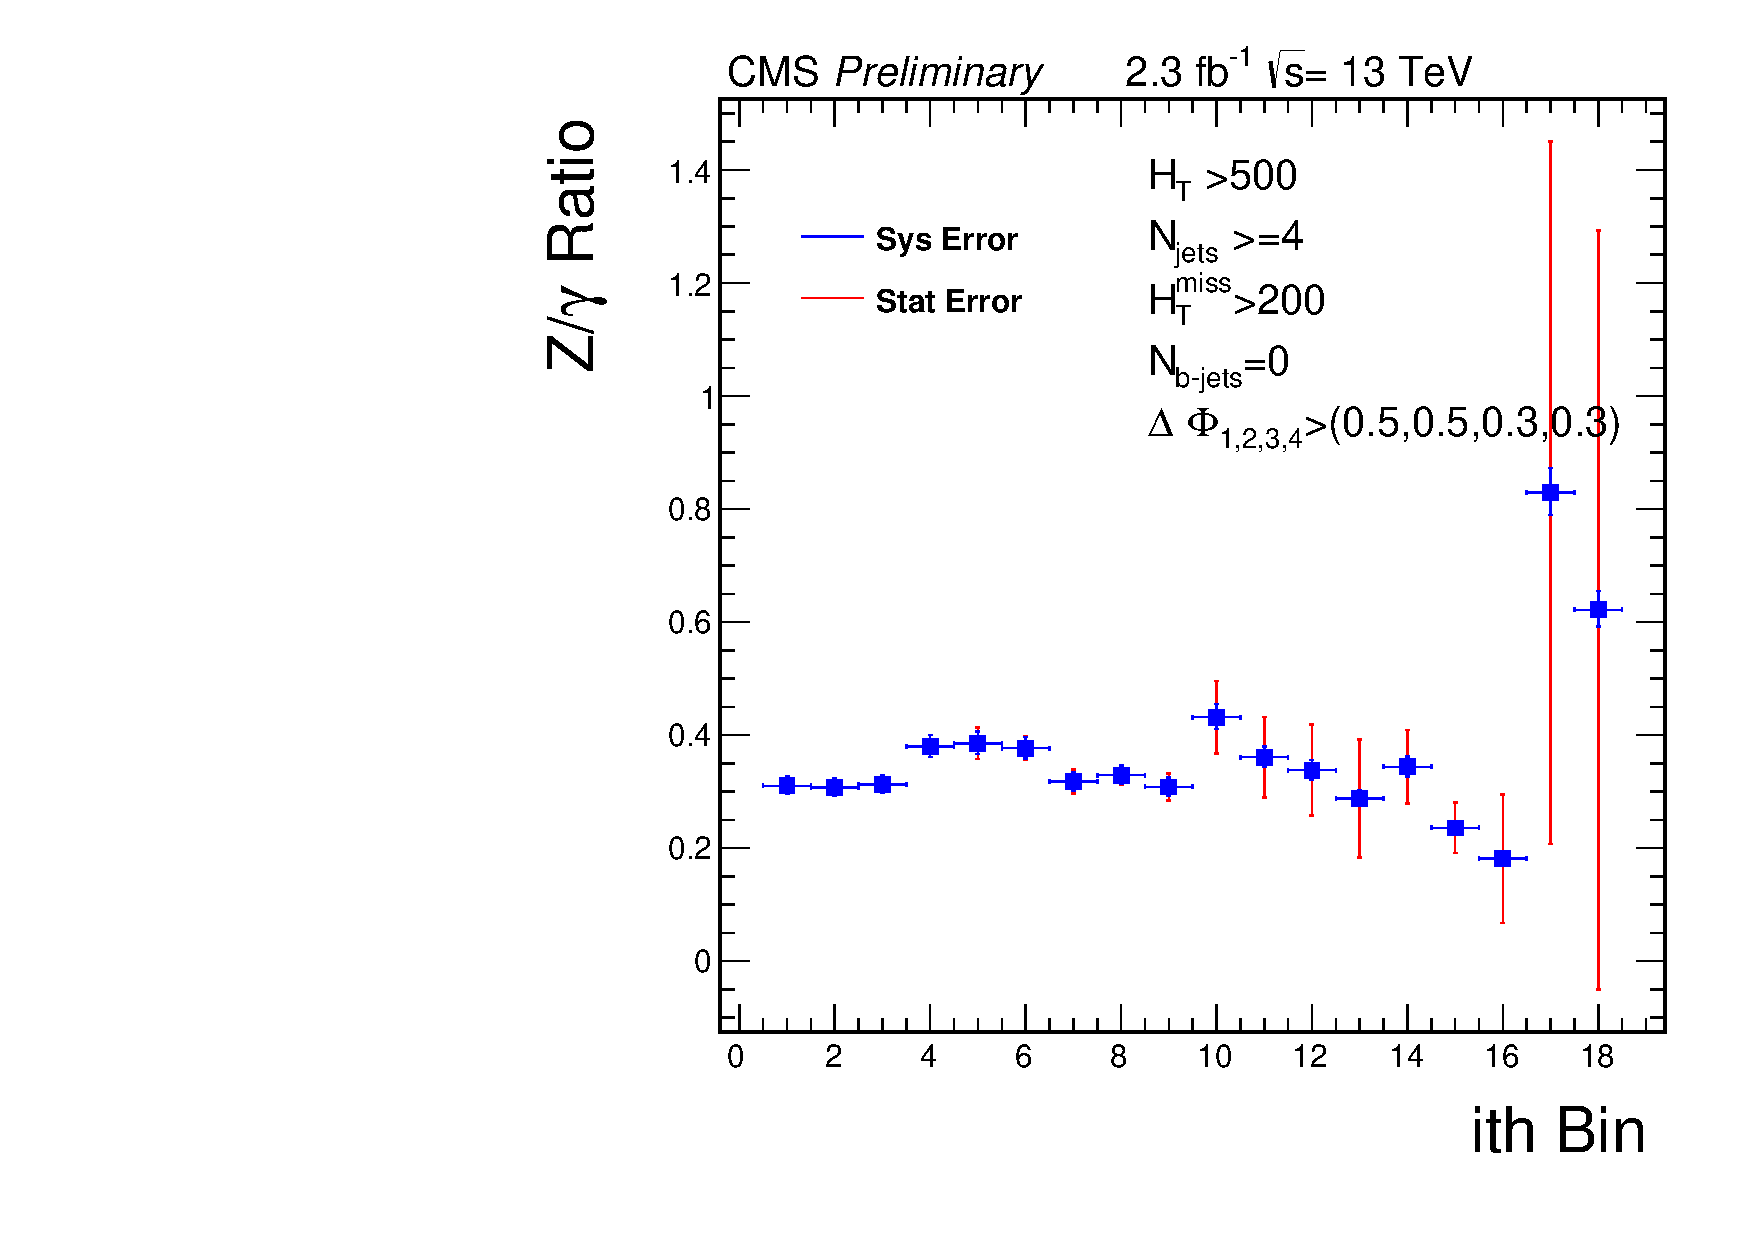
\includegraphics[width=0.48\textwidth]{/home/bibhu/Desktop/PhDThesis/PhDThesis/chapter6/ZGammaRatioWSF.pdf} %ADDNEWPLOT
  \caption{${\cal R}_{Z(\nu\bar{\nu})/\gamma}$ for the 18 analysis bins used in the analysis after baseline selection. The units of $\rm H_{T}$ and $\rm H_{T}^{miss}$  are in GeV.}
  \label{fig:rzg}
\end{center}
\end{figure}

As introduced above, fragmentation photons should be treated carefully when calculating 
${\cal R}_{Z(\nu\bar{\nu})/\gamma}$ primarily because the {\sc MadGraph} $\gamma$+jets events 
that make up the ${\cal R}_{Z(\nu\bar{\nu})/\gamma}$ denominator are generated with the 
requirement that $\Delta R(\gamma,{\rm quarks})>0.4$ and $\Delta R(\gamma,{\rm gluons})>0.4$.
As these fragmentation prompt photons are included in the photon control sample 
and are experimentally indistinguishable from direct prompt photons (unlike non-prompt 
 ones), we must correct for this missing component of the simulation.  We use prompt 
photons included in the QCD simulation sample to determine the fraction with $\Delta R>0.4$. The value of fragmentation fraction is found to be $0.92 \pm 0.08$.








\paragraph{\underline{Lost lepton}: }
The SM events (mostly $\rm t\bar{t}$ and W+jets) with muons or electrons
can satisfy event selection and enter the signal sample as the lost-lepton background
if the requirements for any of the following analysis steps are not satisfied:

\begin{itemize}
\item Kinematic acceptance,
\item Reconstruction, or
\item Isolation.
\end{itemize}
The basic idea behind our data-driven method for calculating
the lost-lepton background is to select
single-lepton control sample (CS) in the data,
through inversion of the lepton vetoes,
and to weight each CS event
by a factor that represents the probability for a lost-lepton event
to appear with
the corresponding search-variables: $\rm H_{T}$, $\rm H_{T}^{miss}$, $\rm N_{jet}$, and $\rm N_{b-jet}$.
The weights are determined through evaluation of the efficiencies
for each analysis step.
The weighted distributions of the search variables,
summed over all CS events,
define the predicted lost-lepton background in the respective search regions.
\paragraph{\underline{QCD}: }
The $\rm H_{T}^{miss}$ in QCD multijet events is almost always due to a mismeasured jet in the event,
       thus the $\rm H_{T}^{miss}$ direction is usually close to the jet.
       The $\rm \Delta \phi$ variable is the minimum azimuthal ($\phi$) difference between $\rm H_{T}^{miss}$ and one of the four
       highest $\rm p_{T}$ jets.


       The low $\rm \Delta \phi$ region is significantly enriched in QCD events.
       The sample of events with the $\rm \Delta \phi$ requirement inverted
       (i.e., $\Delta \phi_1<0.5$ or $\Delta \phi_2<0.5$ or $\Delta \phi_3<0.3$ or $\Delta \phi_4<0.3$)
       serves as the QCD control sample.
       %Figure~\ref{fig:qcd-mdp-split1d} shows \dphi distributions for zero-lepton events
       %passing the baseline selection in bins of \HT, \MHT, and \njets.
       The background at high $\rm \Delta \phi$, is estimated from the QCD yield at low
       $\rm \Delta \phi$ and a high-to-low ratio $R^{\rm QCD}$ for the QCD component.
       The $\rm \Delta \phi$ distribution  shows that the $R^{\rm QCD}$
       has some dependence on the search variables $\rm H_{T}$, $\rm H_{T}^{miss}$, and $\rm N_{jet}$.
       We model this dependence by assuming it factorizes.  That is, we assume the $\rm H_{T}$
       dependence does not depend on $\rm H_{T}^{miss}$ or $\rm N_{jet}$ and vice versa.
\paragraph{\underline{Hadronic tau}: }

To evaluate the $\rm t\bar{t}$, single-top and W+jets backgrounds
that arises when a W boson decays to a hadronically decaying $\tau$ lepton ($\tau^{h}$) and a neutrino,
we employ a tau-template method. %~\cite{RA28TeVpaper,RA28TeVan,RA2-2011pub,RA2-2010pub}.
In this approach, the $\tau^{h}$ background is estimated from a control sample (CS)
of $\mu$+jets events,
which we select by requiring exactly one muon with $\rm p_{T}>20$ GeV and $|\eta|<2.1$. 
This single-muon CS is
mainly composed of $\rm t\bar{t}(\rightarrow \mu\nu)$ and W($\rightarrow \mu\nu$)+jets events.
Since both $\mu$+jets and $\tau^{h}$+jets events 
arise from the same underlying process,
the hadronic components of the two event classes are expected to be the same,
aside from the response of the 
detector to a muon or a $\tau^{h}$ jet. 
The latter effect is incorporated by smearing the muon $\rm p_{T}$ in the CS events,
with MC-derived response functions (the ``templates''),
in order to emulate the $\tau^{h}$ jet response.
Global hadronic variables such as $\rm N_{jet}$, $\rm H_{T}$, and $\rm H_{T}^{miss}$
are then recomputed, with the full analysis procedure being applied. 


\subsection{Results and statistical interpretation}

Here we shall describe the interpretation of the data observed in the signal region vs. all the SM background. Fig ~\ref{fig:dataVsBkg2p3} shows the data vs. the SM backgrounds in the 72 exclusive intervals as defined before.The ratio of likelihood functions, $\mathcal{L} $ is profiled to compute the expected signal significance in units of standard deviations. The likelihood is constructed as the product of Poisson PDFs of observing N events, given a mean n, which depends on the floating parameters in the likelihood. The test statistic used in the profile likelihood calculations is given by \[q_{\mu}=-2\ln\left(\mathcal{L}_{\mu} /\mathcal{L}_{\rm max}\right)\] where the $\mathcal{L}_{\mu}$ is the maximum likelihood at a given signal strength $\mu$ and $\mathcal{L}_{max}$ is the maximum floating all parameters. This test statistic is the same as described in chapter5. The profile likelihood signal significance is given by $\sqrt{q_0}$ (described earlier in sec 5.3) as a number of standard deviations. 

For setting limits, we use the LHC-style $CL_{s}$ ~\cite{CMS-NOTE-2011-005} approach. The $CL_{s}$ ratio is the ratio of confidence intervals:
\[CL_{s}=\frac{CL_{s+b}}{CL_{b}}\]
where $CL_{b}$ is the confidence interval in the background only region and $CL_{s+b}$ is the same in the background region with signal. 
The $95\%$ CL is given by the probability that a test statistic $Q$ is less than the observed value in data: $P_{95\%}\left(Q<Q_{\rm obs}\right)$, 
so it gives a probability of the data being discrepant with the background-only hypothesis. The test statistic $Q$ comes from a modified Profile Likelihood with constraints on the upper bound of the signal strength, so that the method gives an 
upper limit instead of a two-sided limit. The sensitivity of the analysis will scale with the exclusion power, so the $95\%$ CL upper 
exclusion limits will decrease with increasing sensitivity to signal. 

\begin{figure}[h]
\begin{center}
  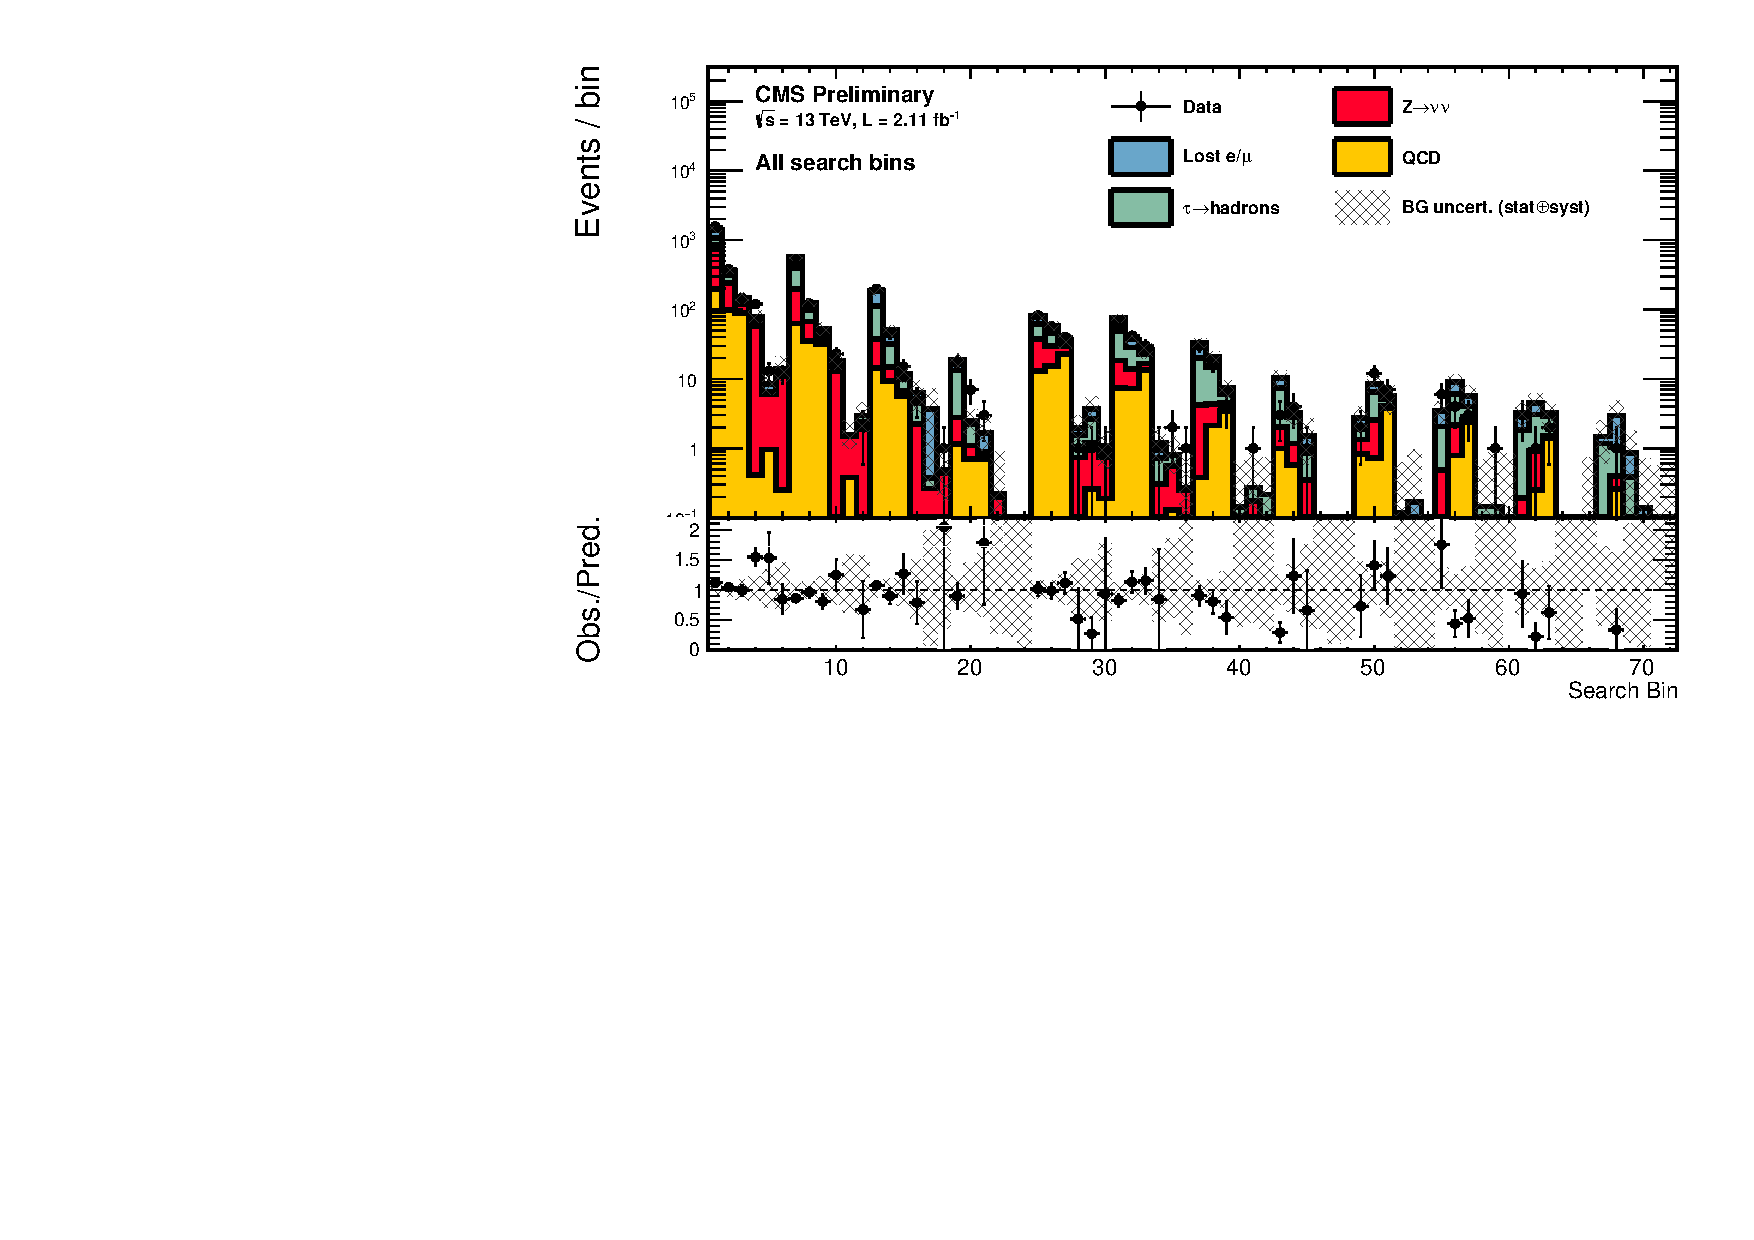
\includegraphics[width=0.78\textwidth]{/home/bibhu/Desktop/PhDThesis/PhDThesis/chapter6/prefit-results-all-log.pdf} %ADDNEWPLOT
  \caption{The observed data vs the SM backgrounds in the 72 exclusive intervals of the signal region. }
  \label{fig:dataVsBkg2p3}
\end{center}
\end{figure}


\begin{figure}[h]
\centering
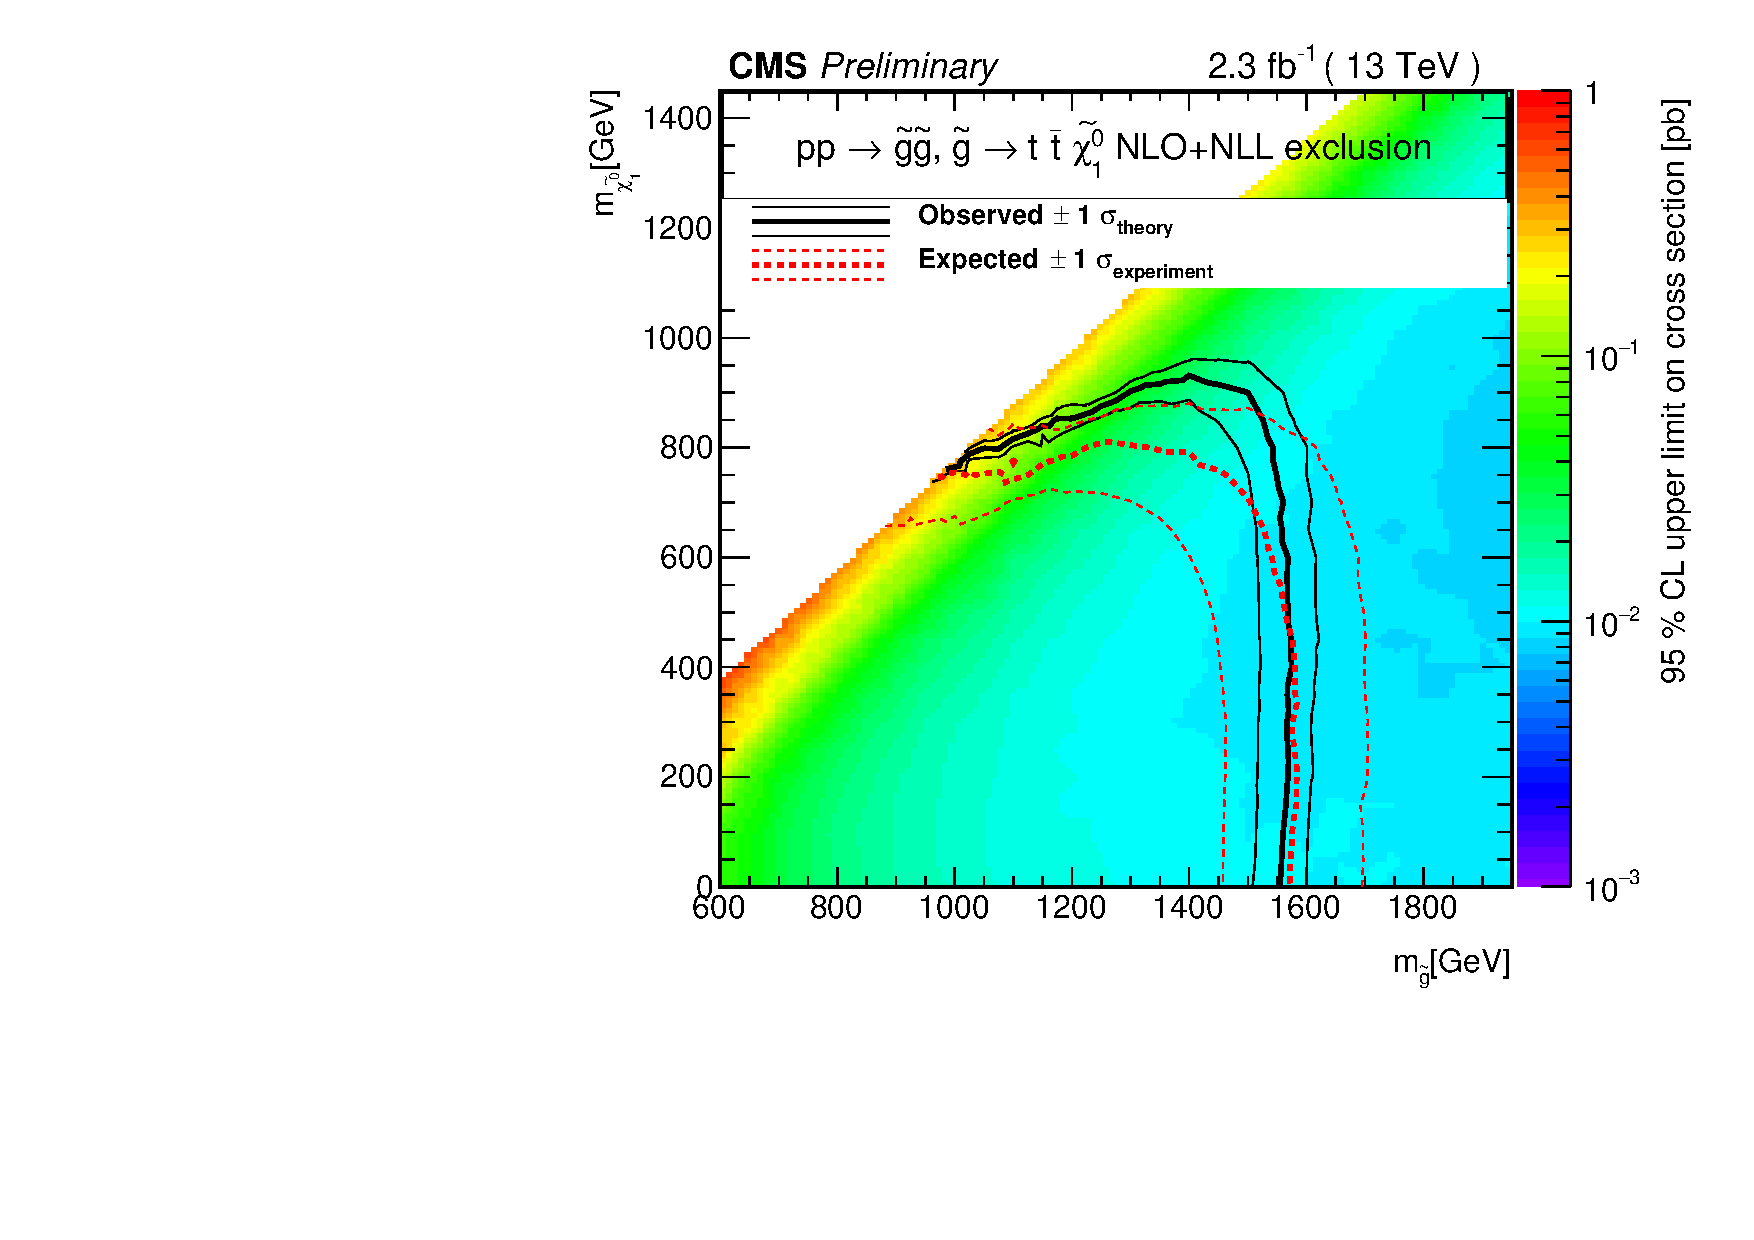
\includegraphics[width=0.32\textwidth]{/home/bibhu/Desktop/PhDThesis/PhDThesis/chapter6/T1tttt_2p3_limit.pdf}
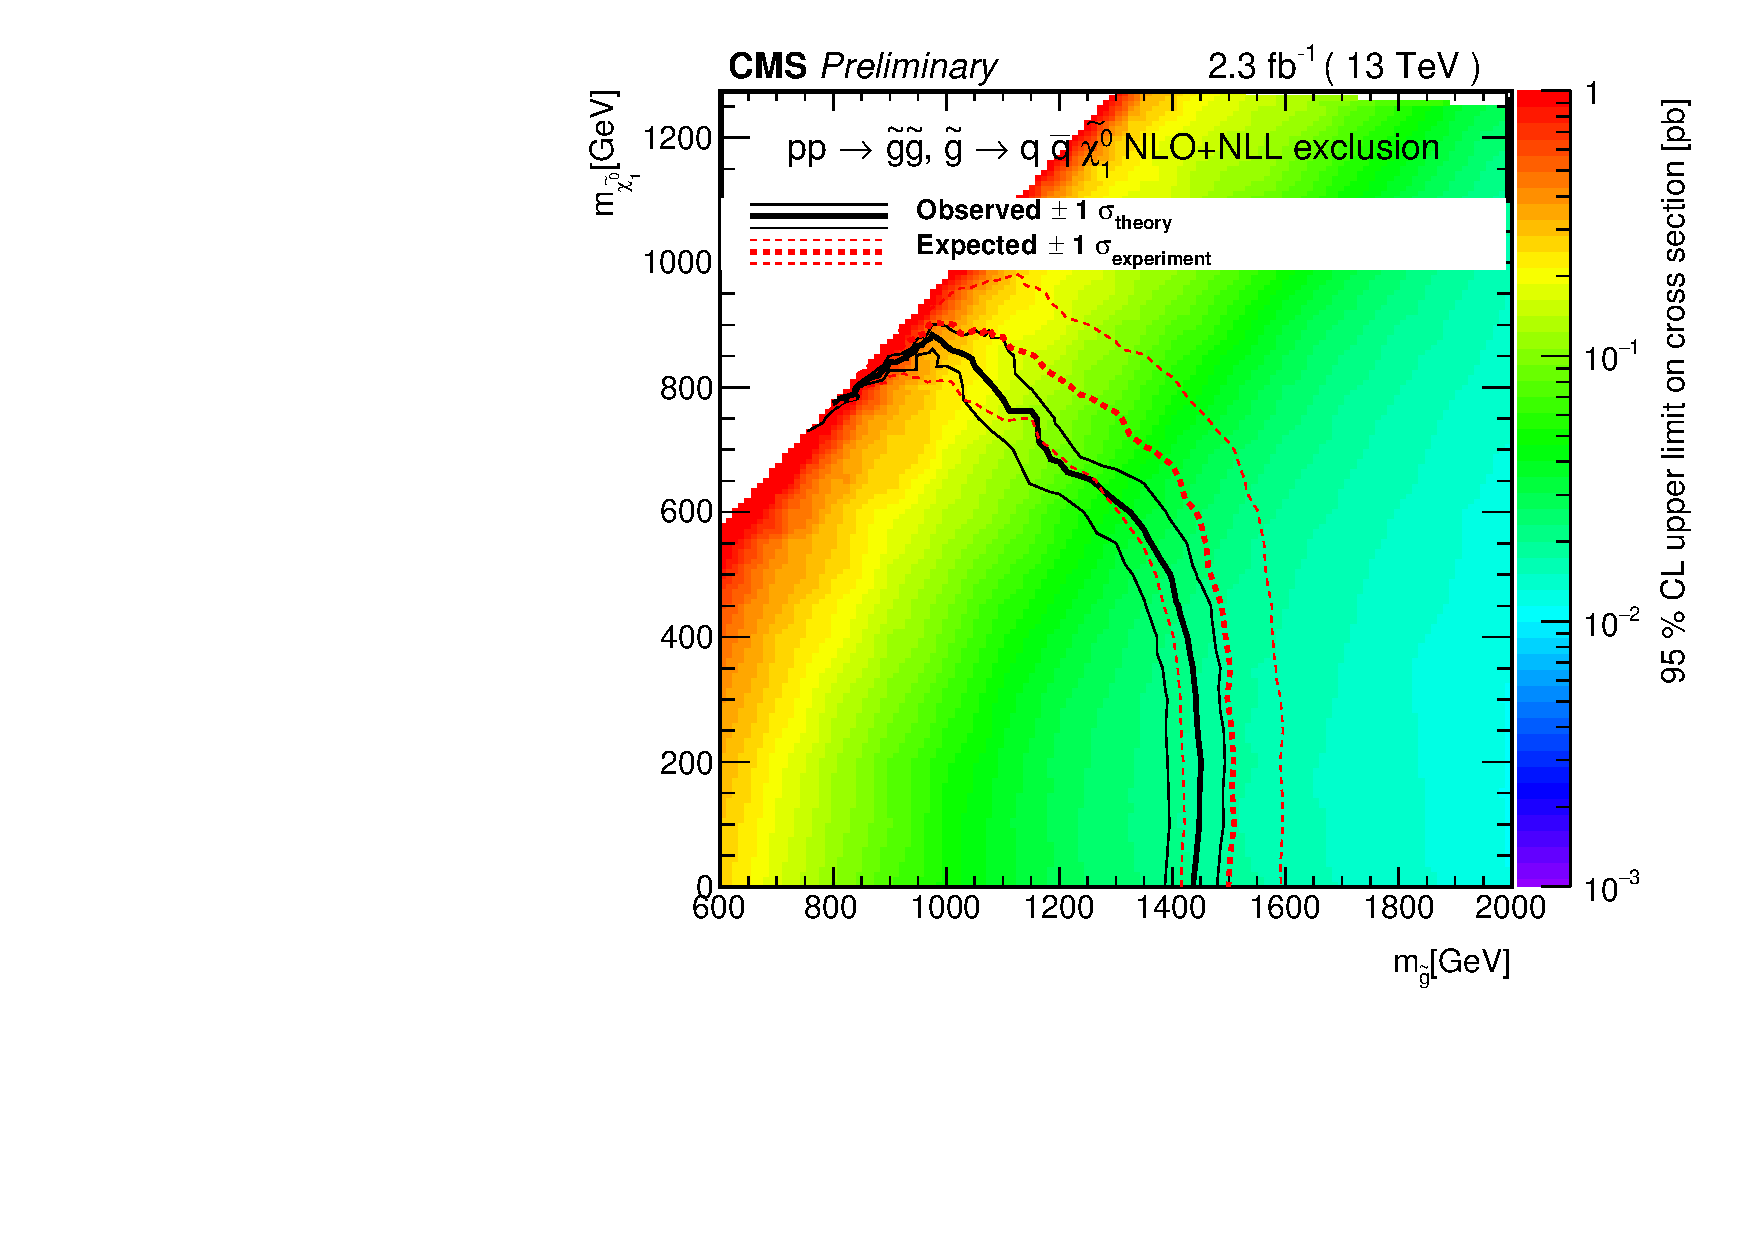
\includegraphics[width=0.32\textwidth]{/home/bibhu/Desktop/PhDThesis/PhDThesis/chapter6/T1qqqq_2p3_limit.pdf}
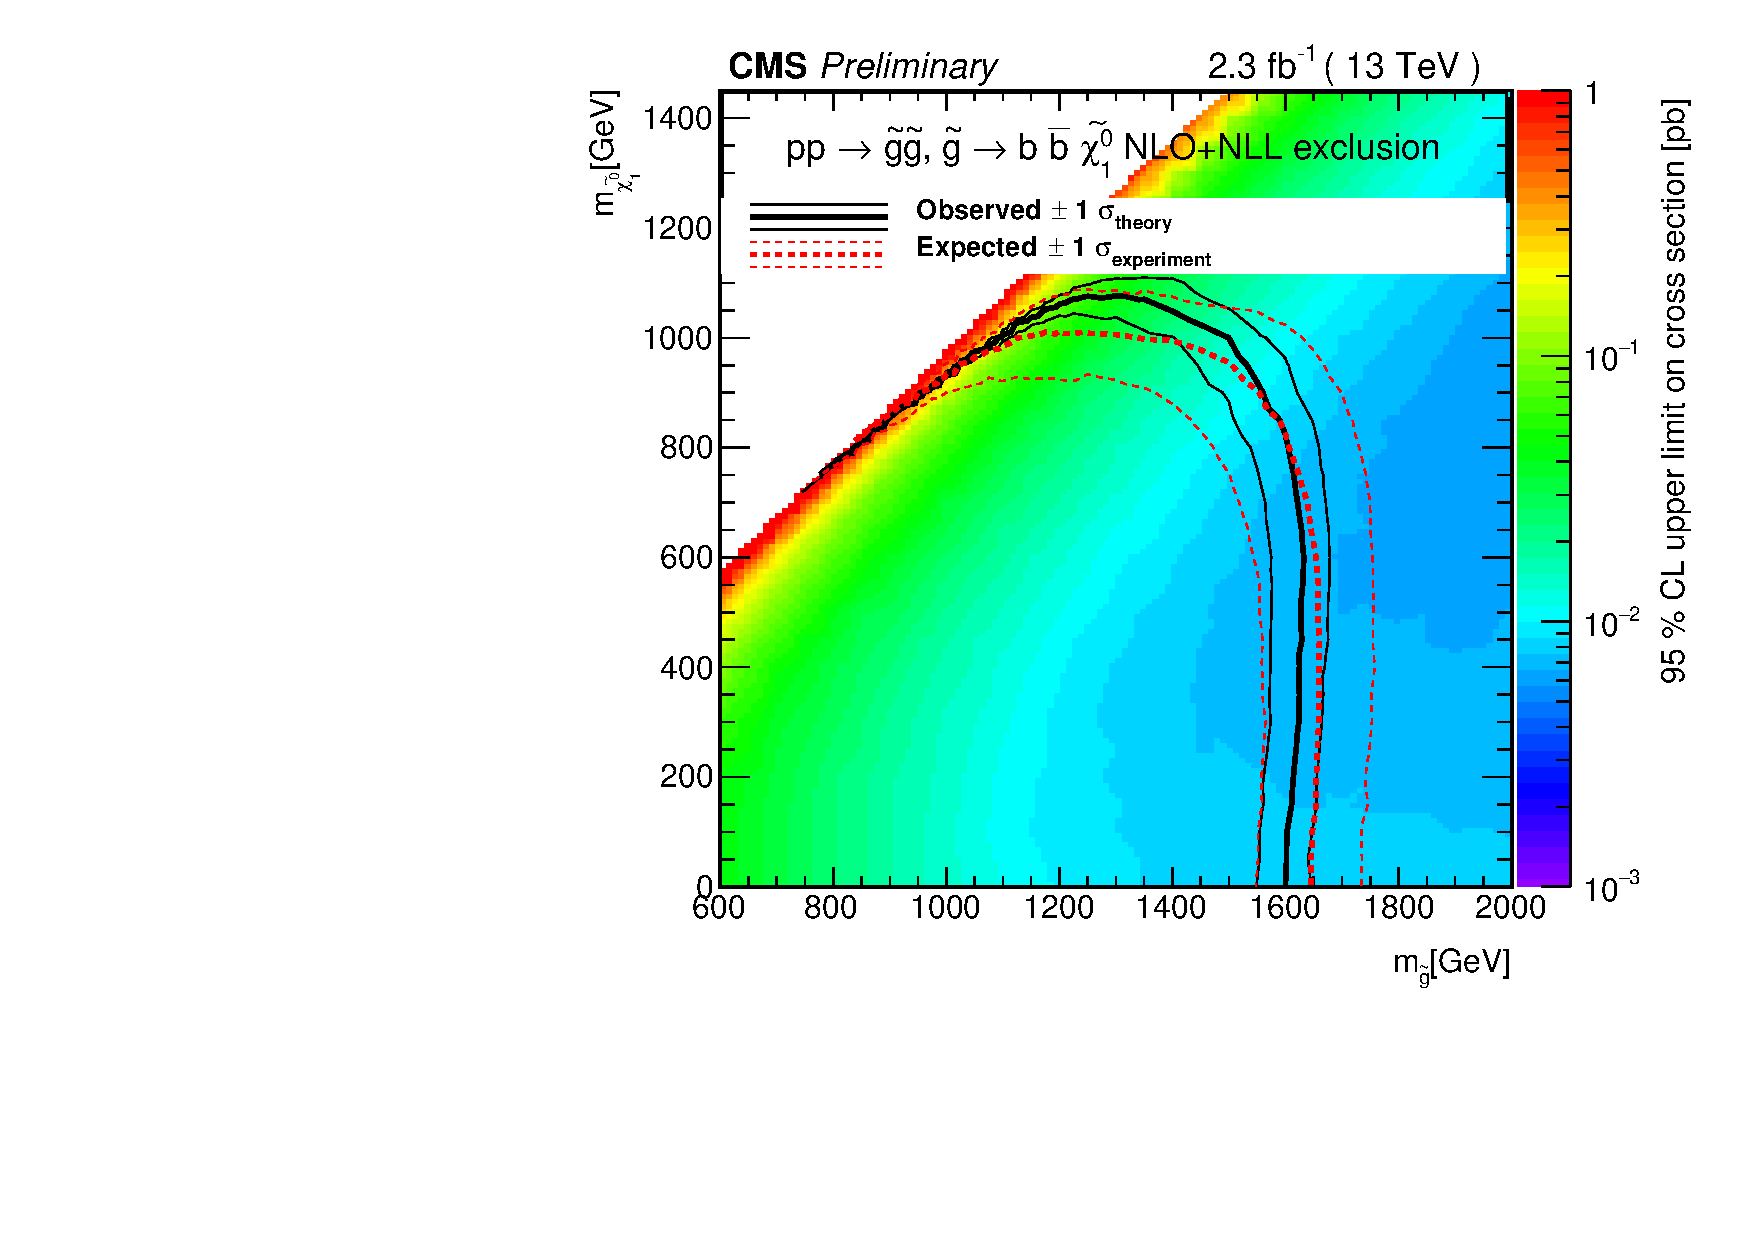
\includegraphics[width=0.32\textwidth]{/home/bibhu/Desktop/PhDThesis/PhDThesis/chapter6/T1bbbb_2p3_limit.pdf}
\caption{\label{fig:Limit2015}The 95\% CL upper limits on the production cross sections for four top quark (left),four light quark (middle) and four b-quark (right) in the final state. }
\end{figure}



\section{Study with 12.9 $\bf \rm fb^{-1}$ of 2016 data}

With the collection of more data in 2016 we update our analysis strategy to enhance the sensistivity. We perform the search in 2016 data using a strategy similar to that used in the 2015 analysis. Therefore, so we will not discuss everything in detail, but rather focus on the major changes before moving over to results. A detailed exposition could be found in Ref.~\cite{CMS-PAS-SUS-16-014}. The three most significant changes to the analysis strategy are:
\begin{itemize}
\item Expanding the search region to include events with 3 or more
  jets. The 2015 analysis considered events with 4 or more
  jets. A more inclusive selection allows us to target  models
  of direct squark production as well as other low-multiplicity signatures.
\item Adopting triggers that make online requirements only on $\rm H_{T}^{miss}$
  and $\rm MET$. The trigger has online PF based MET $>$ 100 and PF based $\rm H_{T}^{miss} > $100.
  These triggers allow us to lower the offline $\rm H_{T}$ threshold from 500 to 300 GeV, giving us increased
  sensitivity to SUSY models with low jet multiplicity or compressed
  spectra.
\item Using a finer binning in $\rm H_{T}$, $\rm H_{T}^{miss}$,
and $\rm N_{jet}$ to take advantage of a much larger dataset in 2016.
\end{itemize}

Apart from these three, there are a number of less important changes in the  background estimation methods. Below we discuss in detail about the changes that occurred to the $Z(\rightarrow \nu \bar{\nu})+$ jets background.


\subsection{Search binning}

As with more data finer bins are possible , we further split the available phase-space into 160 bins in the following way. A schematic diagram in the 2D plane of $\rm H_{T}$ and $\rm H_{T}^{miss}$ is shown in the Fig.~\ref{HTMHT2D2016} 

\begin{itemize}

 \item ${\bf 4 }$ $\rm N_{jet}$ bins: 3-4, 5-6,7-8, $\geq$9; \vspace{-0.2in}
 \item ${\bf 4 }$ $\rm N_{b-jet}$ bins: 0, 1, 2, $\geq$3; and \vspace{-0.2in}
 \item  ${\bf 10 }$ bins in $\rm H_{T}$ and $\rm H_{T}^{miss}$ as defined below:



\begin{center} \label{HTMHT2D2016}
\begin{tabular}{ c c c }
 Bin & $\rm H_{T}$ range [GeV] & $\rm H_{T}^{miss}$ range [GeV] \\ 
  1: & 300-500 & 300-350 \\ 

  2: & 500-1000 & 300-350 \\  

  3: & $>$1000 & 300-350\\

  4:&  350-500 & 350-500\\

  5: & 500-1000 & 350-500\\

  6: & $>$1000 & 350-500\\

  7: & 500-1000 & 500-750\\

  8: & $>$1000 & 500-750\\

  9: & 750-1500 & $>$750\\

 10: & $>$1500 & $>$750\\


\end{tabular}
\end{center}

\end{itemize}
 

\begin{figure}[h]
\begin{center}
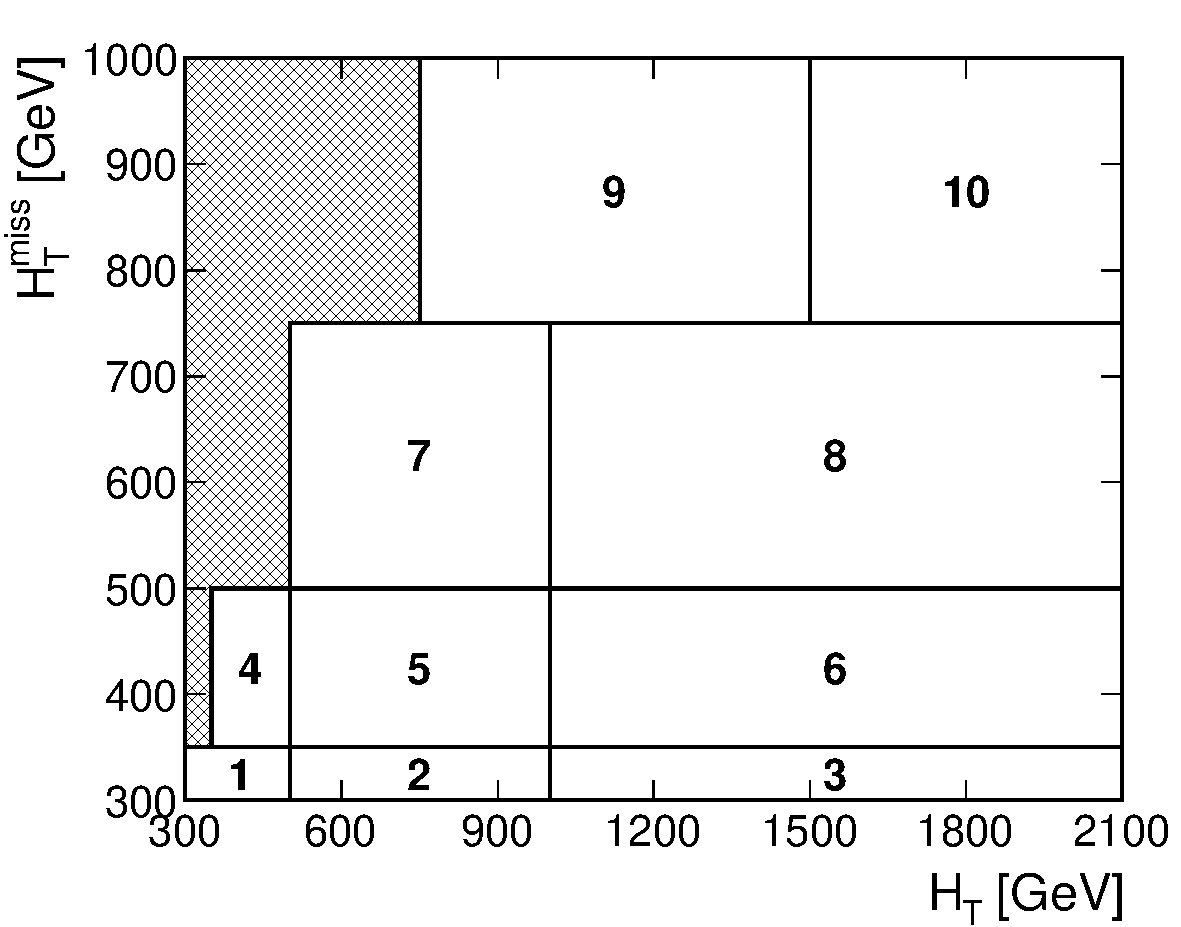
\includegraphics[width=0.45\textwidth]{/home/bibhu/Desktop/PhDThesis/PhDThesis/chapter6/HT-MHT-2016.pdf}

\caption{\label{fig:HT-MHT-2016} Search binning in the 2D phane of $\rm H_{T}$ and $\rm H_{T}^{miss}$ used in the 2016 analysis.}
\end{center}
\end{figure}



\subsection{\bf $\bf Z(\rightarrow \nu \bar{\nu})+$ jets background estimation}


Our baseline strategy is the same as that used in the 2015 search discussed earlier.
We use the $\rm \gamma +$jets sample to determine the
yields in the 40 bins corresponding to $\rm N_{b-jet}=0$.  These are
 then compared with the Z($\rightarrow \ell^{+} \ell^{-}$) yields in the low-$\rm N_{jet}$
bin to establish the systematic uncertainty of the physics modeling of
$\rm \gamma +$ jets, and the normalization corrected if necessary.  
The extrapolation to bins with $\rm N_{b-jet}>0$ is performed to
the extent possible with the Z($\rightarrow \ell^{+} \ell^{-}$) data sample, supplemented with MC
information where necessary.  The photon (dilepton) samples require a
photon (dilepton) candidate with $\rm p_{T}>200 GeV$. The increase in the $\rm p_{T}$ cut is due to trigger reasons. We show the data vs. MC expectation in the 40  0-btagged bins in the Fig.~\ref{fig:nobs2016}. In the table ~\ref{tab:gjets_res} we present the estimated Z background in those 40 bins.


\begin{figure}[h]
\begin{center}
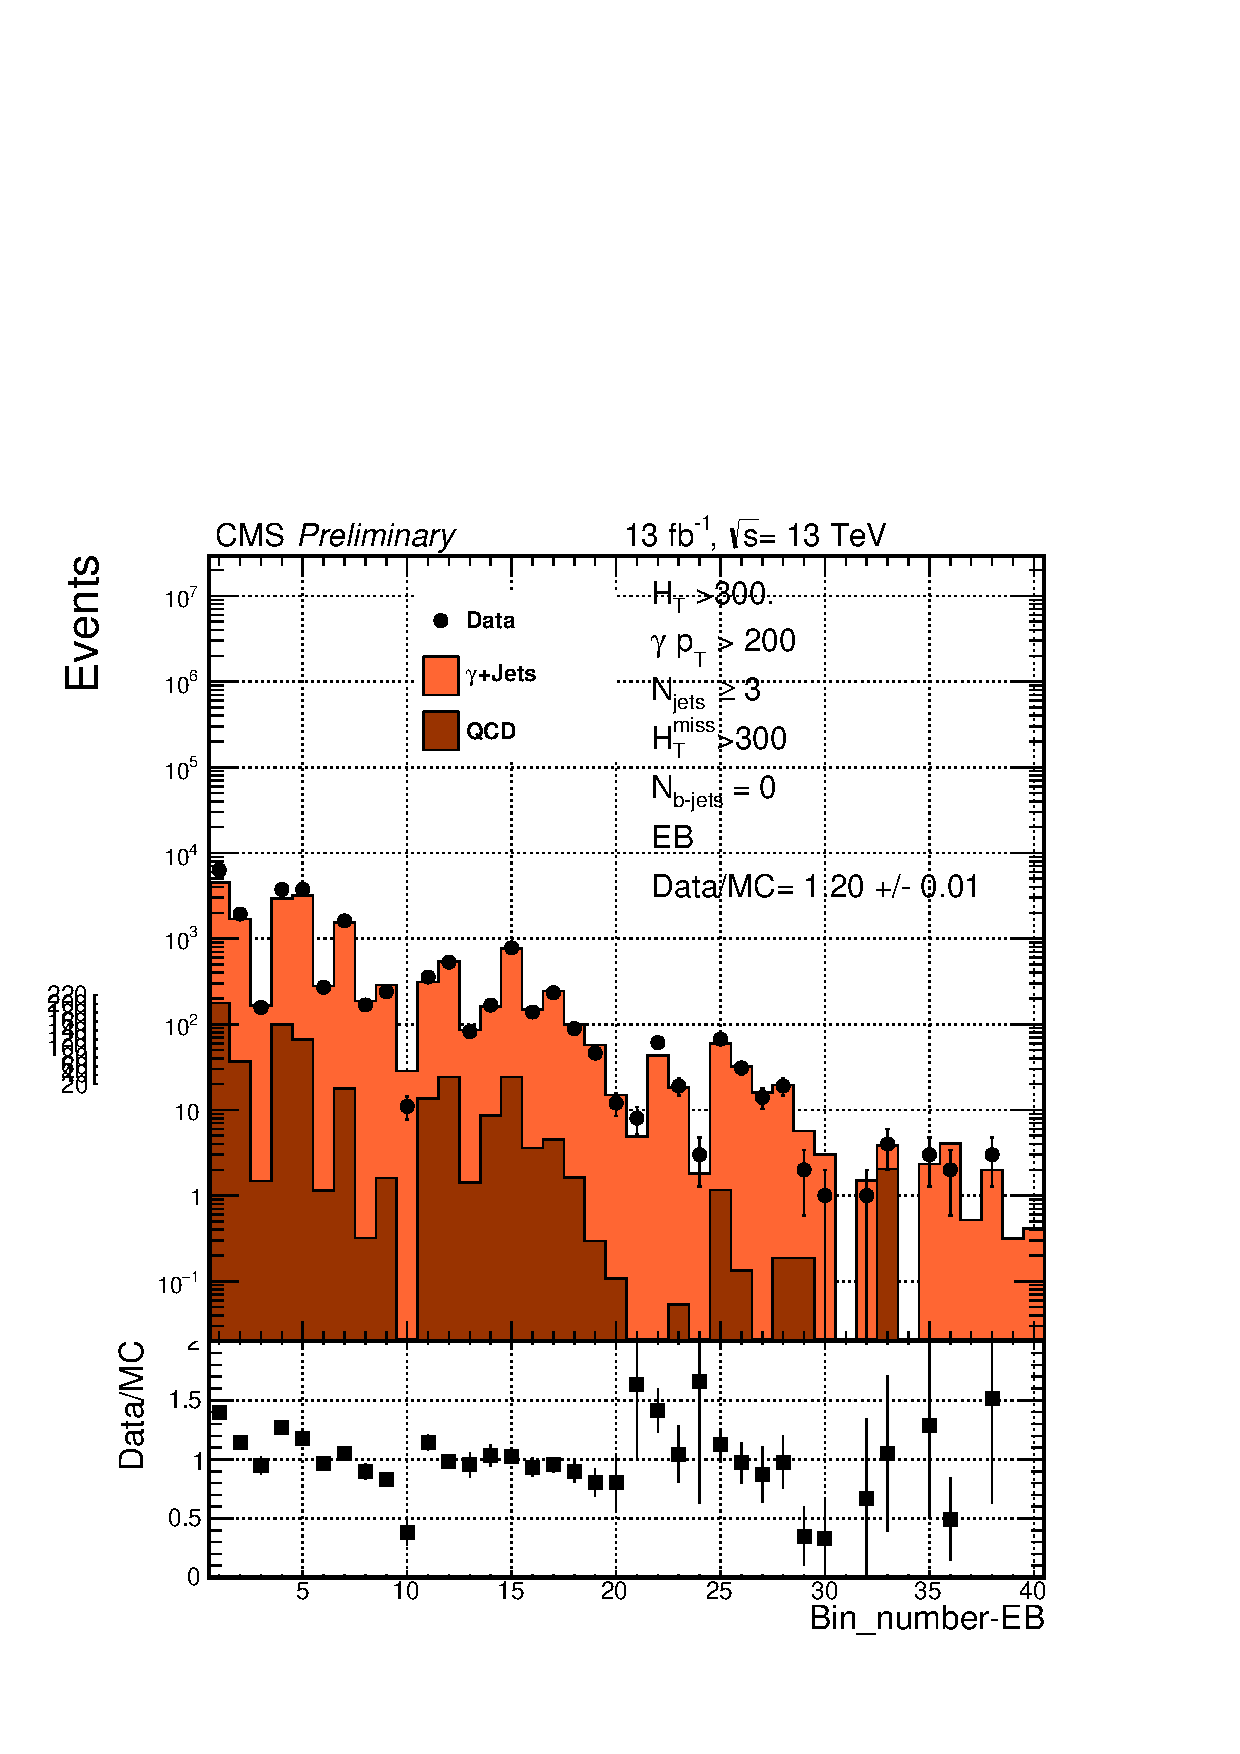
\includegraphics[width=0.48\textwidth]{/home/bibhu/Desktop/PhDThesis/PhDThesis/chapter6/ith-Bin-EB__Data_MC_EB2016.pdf} % ADDNEWPLOT 
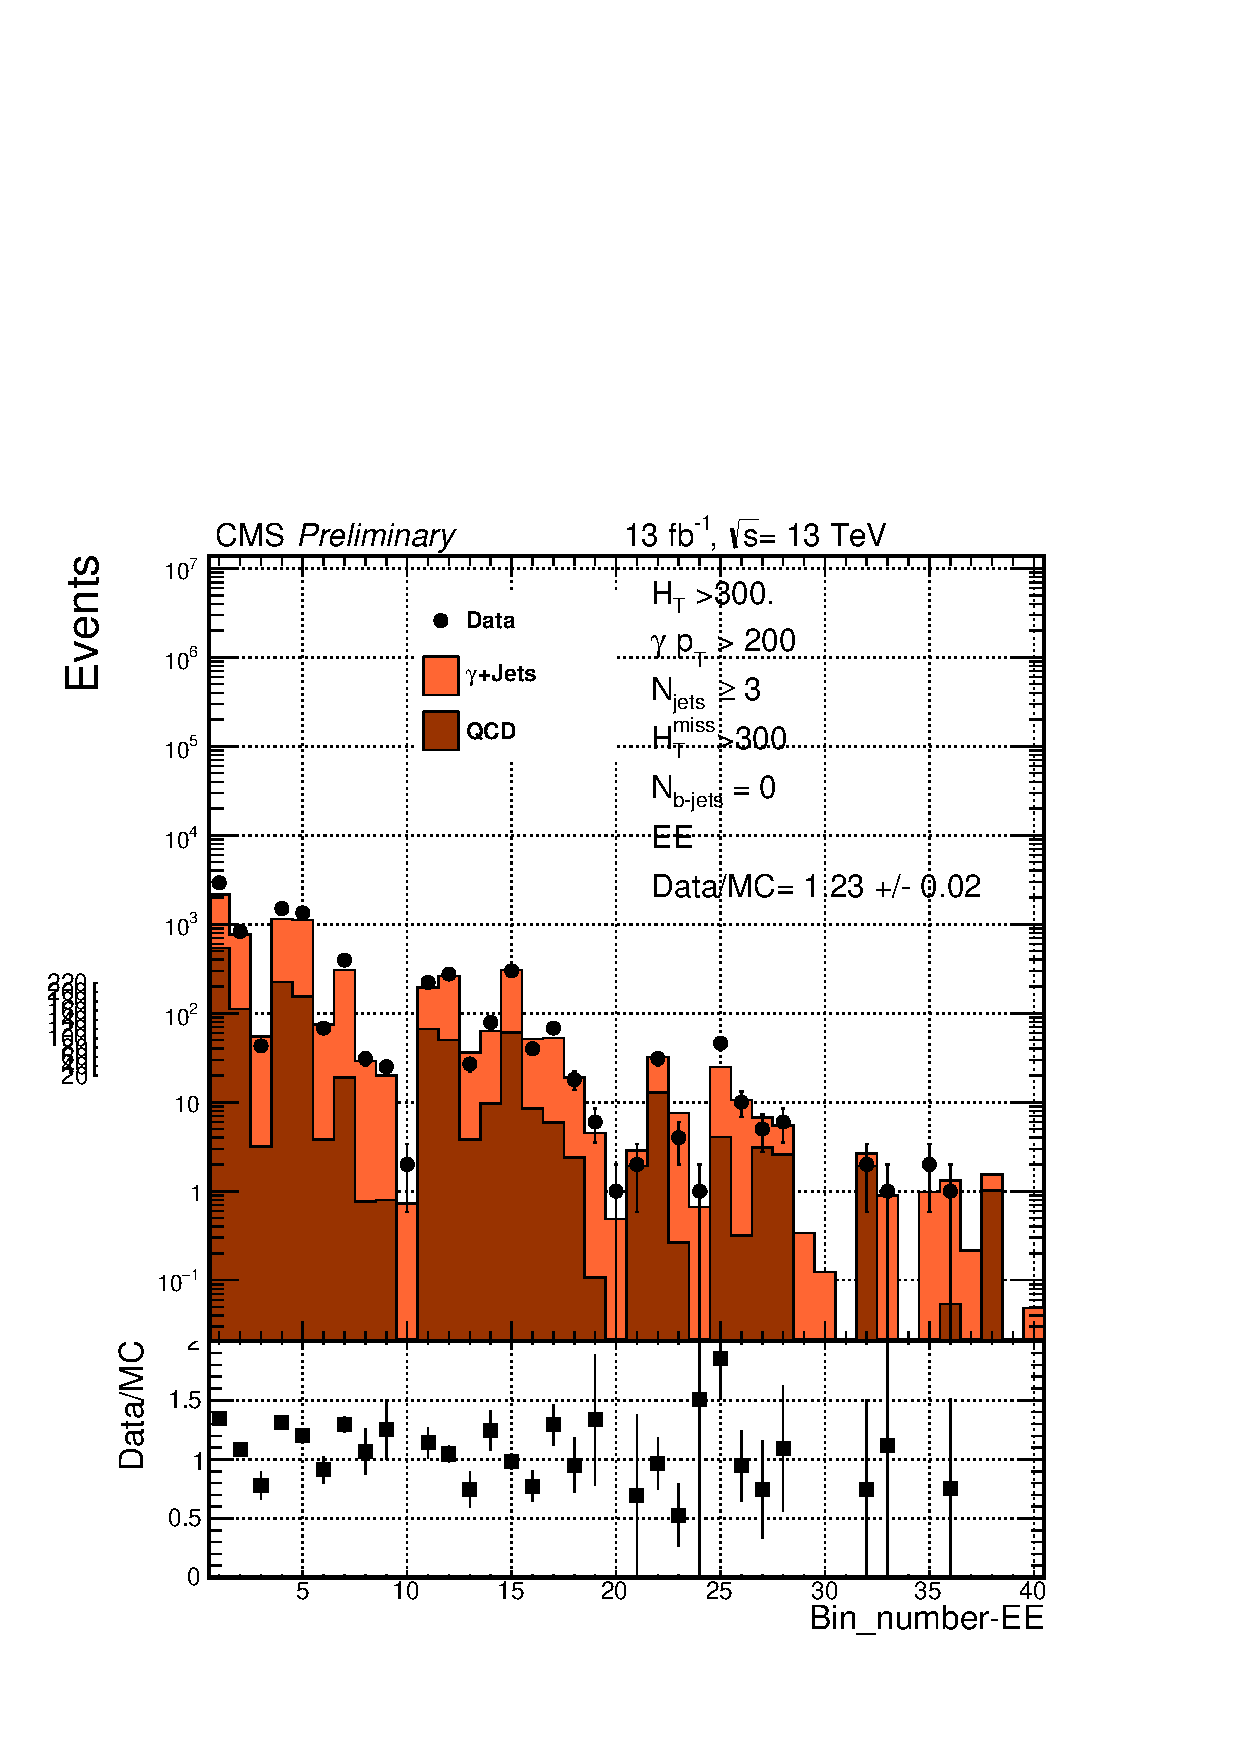
\includegraphics[width=0.48\textwidth]{/home/bibhu/Desktop/PhDThesis/PhDThesis/chapter6/ith-Bin-EE__Data_MC_EE2016.pdf} % ADDNEWPLOT 
\caption{Numbers of observed events in the photon control samples in EB (left) and EE (right) compared to simulation. The units of $\rm H_{T}$ and $H_{T}^{miss}$ are in GeV.}
\label{fig:nobs2016}
\end{center}
\end{figure}




%%%%%%%%%%%%%%%%%%%%%%%%%



\begin{table}[h]
%\begin{center}
\caption{$Z\to\nu\nu$+jets prediction ($N_{Z\to\nu\nu}^{\rm pred}$) in
  the 40 0-btag analysis bins as determined with the $\gamma +$jets method.  We
  show the inputs to the determination of $N_{Z\to\nu\nu}^{\rm pred}$ as
   that vary for the 40 bins, including
  $N_{\gamma}^{\rm obs}$ in EB and EE, $R_{Z/\gamma}$, and double ratio. The first
  uncertainty on $R_{Z/\gamma}$ comes from the statistical uncertainty on the
  simulation and the second from
  variation of the data-MC scale factors for photon reconstruction, ID,
  and isolation.  
%% The purity and direct prompt fraction are described in the text.
}
\label{tab:gjets_res}
\hspace{-0.50in}\begin{tabular}{|c|rr|c|c|r|}
\hline
Bin & $N_{\gamma, {\rm EB}}^{\rm obs}$ & $N_{\gamma, {\rm EE}}^{\rm obs}$ & $R_{Z/\gamma}$ & Double ratio  &  $N_{Z\to\nu\nu}^{\rm pred}$ \\
\hline
 1 ($N_{\rm jet}$ 3-4, MHT\_HT\_1)    & 6287 &  2935 & $0.413\pm0.004^{+0.022}_{-0.020}$ & $0.966\pm0.032^{+0.024}_{-0.000}$ & $3146.2\pm32.8^{+216.6}_{-189.5}$ \\  
 2 ($N_{\rm jet}$ 3-4, MHT\_HT\_2)    & 1936 &   830 & $0.374\pm0.004^{+0.020}_{-0.018}$ & $0.966\pm0.032^{+0.022}_{-0.000}$ & $ 856.5\pm16.3^{+58.6}_{-51.7}$ \\      
 3 ($N_{\rm jet}$ 3-4, MHT\_HT\_3)    &  157 &    43 & $0.378\pm0.007^{+0.020}_{-0.018}$ & $0.966\pm0.032^{+0.122}_{-0.089}$ & $  63.0\pm 4.5^{+ 9.0}_{- 7.0}$ \\      
 4 ($N_{\rm jet}$ 3-4, MHT\_HT\_4)    & 3747 &  1502 & $0.430\pm0.005^{+0.023}_{-0.021}$ & $0.966\pm0.032^{+0.021}_{-0.000}$ & $1910.2\pm26.4^{+122.5}_{-106.8}$ \\  
 5 ($N_{\rm jet}$ 3-4, MHT\_HT\_5)    & 3749 &  1347 & $0.407\pm0.004^{+0.022}_{-0.020}$ & $0.966\pm0.032^{+0.018}_{-0.000}$ & $1757.4\pm24.6^{+110.2}_{-97.2}$ \\     
 6 ($N_{\rm jet}$ 3-4, MHT\_HT\_6)    &  270 &    68 & $0.403\pm0.006^{+0.021}_{-0.019}$ & $0.966\pm0.032^{+0.122}_{-0.089}$ & $ 115.9\pm 6.3^{+16.3}_{-12.5}$ \\      
 7 ($N_{\rm jet}$ 3-4, MHT\_HT\_7)    & 1612 &   396 & $0.429\pm0.004^{+0.023}_{-0.021}$ & $0.966\pm0.032^{+0.062}_{-0.033}$ & $ 749.9\pm16.7^{+63.8}_{-46.3}$ \\      
 8 ($N_{\rm jet}$ 3-4, MHT\_HT\_8)    &  168 &    31 & $0.451\pm0.008^{+0.024}_{-0.022}$ & $0.966\pm0.032^{+0.122}_{-0.089}$ & $  78.3\pm 5.6^{+10.9}_{- 8.3}$ \\      
 9 ($N_{\rm jet}$ 3-4, MHT\_HT\_9)    &  240 &    25 & $0.443\pm0.006^{+0.023}_{-0.021}$ & $0.966\pm0.032^{+0.160}_{-0.102}$ & $ 102.6\pm 6.3^{+17.9}_{-12.1}$ \\      
 10 ($N_{\rm jet}$ 3-4, MHT\_HT\_10)  &   11 &     2 & $0.515\pm0.025^{+0.027}_{-0.025}$ & $0.966\pm0.032^{+0.209}_{-0.156}$ & $   5.8\pm 1.6^{+ 1.3}_{- 1.0}$ \\      
\hline                                 															      
 11 ($N_{\rm jet}$ 5-6, MHT\_HT\_1)   &  355 &   222 & $0.393\pm0.015^{+0.021}_{-0.019}$ & $0.966\pm0.032^{+0.059}_{-0.033}$ & $ 186.4\pm 7.8^{+17.8}_{-14.5}$ \\      
 12 ($N_{\rm jet}$ 5-6, MHT\_HT\_2)   &  530 &   276 & $0.382\pm0.008^{+0.020}_{-0.018}$ & $0.966\pm0.032^{+0.059}_{-0.033}$ & $ 254.0\pm 8.9^{+23.0}_{-18.2}$ \\      
 13 ($N_{\rm jet}$ 5-6, MHT\_HT\_3)   &   82 &    27 & $0.375\pm0.009^{+0.020}_{-0.018}$ & $0.966\pm0.032^{+0.122}_{-0.089}$ & $  34.0\pm 3.3^{+ 4.9}_{- 3.8}$ \\      
 14 ($N_{\rm jet}$ 5-6, MHT\_HT\_4)   &  167 &    79 & $0.357\pm0.020^{+0.019}_{-0.017}$ & $0.966\pm0.032^{+0.059}_{-0.033}$ & $  74.1\pm 4.7^{+ 7.5}_{- 6.3}$ \\      
 15 ($N_{\rm jet}$ 5-6, MHT\_HT\_5)   &  780 &   300 & $0.410\pm0.007^{+0.022}_{-0.020}$ & $0.966\pm0.032^{+0.059}_{-0.033}$ & $ 374.8\pm11.4^{+32.5}_{-25.0}$ \\      
 16 ($N_{\rm jet}$ 5-6, MHT\_HT\_6)   &  139 &    40 & $0.415\pm0.008^{+0.022}_{-0.020}$ & $0.966\pm0.032^{+0.122}_{-0.089}$ & $  63.1\pm 4.7^{+ 8.9}_{- 6.9}$ \\      
 17 ($N_{\rm jet}$ 5-6, MHT\_HT\_7)   &  234 &    68 & $0.422\pm0.009^{+0.022}_{-0.020}$ & $0.966\pm0.032^{+0.062}_{-0.033}$ & $ 110.8\pm 6.4^{+ 9.7}_{- 7.2}$ \\      
 18 ($N_{\rm jet}$ 5-6, MHT\_HT\_8)   &   89 &    18 & $0.449\pm0.011^{+0.024}_{-0.022}$ & $0.966\pm0.032^{+0.122}_{-0.089}$ & $  41.9\pm 4.0^{+ 5.9}_{- 4.5}$ \\      
 19 ($N_{\rm jet}$ 5-6, MHT\_HT\_9)   &   46 &     6 & $0.442\pm0.015^{+0.023}_{-0.021}$ & $0.966\pm0.032^{+0.160}_{-0.102}$ & $  20.1\pm 2.8^{+ 3.6}_{- 2.4}$ \\      
 20 ($N_{\rm jet}$ 5-6, MHT\_HT\_10)  &   12 &     1 & $0.462\pm0.031^{+0.024}_{-0.022}$ & $0.966\pm0.032^{+0.209}_{-0.156}$ & $   5.3\pm 1.5^{+ 1.2}_{- 1.0}$ \\      
\hline                                 															      
 21 ($N_{\rm jet}$ 7-8, MHT\_HT\_1)   &    8 &     2 & $0.454\pm0.126^{+0.024}_{-0.022}$ & $0.966\pm0.032^{+0.127}_{-0.085}$ & $   3.8\pm 1.2^{+ 1.2}_{- 1.1}$ \\      
 22 ($N_{\rm jet}$ 7-8, MHT\_HT\_2)   &   61 &    31 & $0.375\pm0.025^{+0.020}_{-0.018}$ & $0.966\pm0.032^{+0.127}_{-0.085}$ & $  28.5\pm 3.0^{+ 4.6}_{- 3.6}$ \\      
 23 ($N_{\rm jet}$ 7-8, MHT\_HT\_3)   &   19 &     4 & $0.410\pm0.021^{+0.022}_{-0.020}$ & $0.966\pm0.032^{+0.127}_{-0.089}$ & $   7.9\pm 1.6^{+ 1.2}_{- 1.0}$ \\      
 24 ($N_{\rm jet}$ 7-8, MHT\_HT\_4)   &    3 &     1 & $0.688\pm0.319^{+0.036}_{-0.033}$ & $0.966\pm0.032^{+0.127}_{-0.085}$ & $   2.3\pm 1.2^{+ 1.1}_{- 1.1}$ \\      
 25 ($N_{\rm jet}$ 7-8, MHT\_HT\_5)   &   67 &    46 & $0.407\pm0.022^{+0.022}_{-0.020}$ & $0.966\pm0.032^{+0.127}_{-0.085}$ & $  38.6\pm 3.6^{+ 6.0}_{- 4.5}$ \\      
 26 ($N_{\rm jet}$ 7-8, MHT\_HT\_6)   &   31 &    10 & $0.421\pm0.017^{+0.022}_{-0.020}$ & $0.966\pm0.032^{+0.127}_{-0.089}$ & $  14.6\pm 2.3^{+ 2.2}_{- 1.7}$ \\      
 27 ($N_{\rm jet}$ 7-8, MHT\_HT\_7)   &   14 &     5 & $0.411\pm0.032^{+0.022}_{-0.020}$ & $0.966\pm0.032^{+0.127}_{-0.085}$ & $   6.8\pm 1.6^{+ 1.1}_{- 0.9}$ \\      
 28 ($N_{\rm jet}$ 7-8, MHT\_HT\_8)   &   19 &     6 & $0.474\pm0.026^{+0.025}_{-0.023}$ & $0.966\pm0.032^{+0.127}_{-0.089}$ & $  10.3\pm 2.1^{+ 1.6}_{- 1.2}$ \\      
 29 ($N_{\rm jet}$ 7-8, MHT\_HT\_9)   &    2 &     0 & $0.502\pm0.053^{+0.027}_{-0.024}$ & $0.966\pm0.032^{+0.160}_{-0.102}$ & $   0.9\pm 0.6^{+ 0.2}_{- 0.1}$ \\      
 30 ($N_{\rm jet}$ 7-8, MHT\_HT\_10)  &    1 &     0 & $0.458\pm0.066^{+0.024}_{-0.022}$ & $0.966\pm0.032^{+0.209}_{-0.156}$ & $   0.4\pm 0.4^{+ 0.1}_{- 0.1}$ \\      
\hline                                 															      
 31 ($N_{\rm jet}$ 9+, MHT\_HT\_1)    &    0 &     0 & $0.455\pm0.202^{+0.024}_{-0.022}$ & $0.966\pm0.032^{+0.193}_{-0.133}$ & $   0.4\pm 0.4^{+ 0.2}_{- 0.2}$ \\    
 32 ($N_{\rm jet}$ 9+, MHT\_HT\_2)    &    1 &     2 & $0.268\pm0.054^{+0.014}_{-0.013}$ & $0.966\pm0.032^{+0.193}_{-0.133}$ & $   0.6\pm 0.4^{+ 0.2}_{- 0.2}$ \\      
 33 ($N_{\rm jet}$ 9+, MHT\_HT\_3)    &    4 &     1 & $0.565\pm0.086^{+0.030}_{-0.027}$ & $0.966\pm0.032^{+0.193}_{-0.133}$ & $   2.4\pm 1.1^{+ 0.6}_{- 0.5}$ \\      
 34 ($N_{\rm jet}$ 9+, MHT\_HT\_4)    &    0 &     0 & $0.455\pm0.202^{+0.024}_{-0.022}$ & $0.966\pm0.032^{+0.193}_{-0.133}$ & $   0.4\pm 0.4^{+ 0.2}_{- 0.2}$ \\      
 35 ($N_{\rm jet}$ 9+, MHT\_HT\_5)    &    3 &     2 & $0.364\pm0.064^{+0.019}_{-0.017}$ & $0.966\pm0.032^{+0.193}_{-0.133}$ & $   1.5\pm 0.7^{+ 0.4}_{- 0.4}$ \\      
 36 ($N_{\rm jet}$ 9+, MHT\_HT\_6)    &    2 &     1 & $0.430\pm0.049^{+0.023}_{-0.021}$ & $0.966\pm0.032^{+0.193}_{-0.133}$ & $   1.1\pm 0.6^{+ 0.3}_{- 0.2}$ \\      
 37 ($N_{\rm jet}$ 9+, MHT\_HT\_7)    &    0 &     0 & $0.258\pm0.082^{+0.014}_{-0.012}$ & $0.966\pm0.032^{+0.193}_{-0.133}$ & $   0.2\pm 0.2^{+ 0.1}_{- 0.1}$ \\      
 38 ($N_{\rm jet}$ 9+, MHT\_HT\_8)    &    3 &     0 & $0.484\pm0.079^{+0.026}_{-0.023}$ & $0.966\pm0.032^{+0.193}_{-0.133}$ & $   1.3\pm 0.7^{+ 0.3}_{- 0.3}$ \\      
 39 ($N_{\rm jet}$ 9+, MHT\_HT\_9)    &    0 &     0 & $0.265\pm0.109^{+0.014}_{-0.013}$ & $0.966\pm0.032^{+0.193}_{-0.133}$ & $   0.2\pm 0.2^{+ 0.1}_{- 0.1}$ \\      
 40 ($N_{\rm jet}$ 9+, MHT\_HT\_10)   &    0 &     0 & $0.350\pm0.134^{+0.019}_{-0.017}$ & $0.966\pm0.032^{+0.209}_{-0.156}$ & $   0.3\pm 0.3^{+ 0.1}_{- 0.1}$ \\    
\hline
\end{tabular}
%\end{center}
\end{table}



The background estimated from $\gamma +$jets are used to extrapolate to higher b-tagged bins using a method described in Ref.~\cite{CMS-PAS-SUS-16-014}. Without discussing further on other background methods, we will go to result directly. 

%%%%%%%%%%%%%%%%%%%%%%%%%%%%%%%%





\subsection{Results and statistical interpretation}
This section contains the results of the search. The observations in the signal regions are found to be in 
generally good agreement with the predicted backgrounds. For the 160
search bins, the observed data and the pre-fit predictions for each background
component are shown in Fig.~\ref{fig:DataVsBkg2016}. The statistical procedures used to calculate limtis are the same as decribed in the chapter 5. The upper limits on the signal strengths are shown in Fig.~\ref{fig:Limit2016}. The statistical procedures followed to obtain the limits are exactly the same as is done for the previous analysis. As could be see from the Fig ~\ref{fig:DataVsBkg2016}, no significant excess is found from the SM expectations. For the simplified models considered here, we exlude gluino masses up to in the range 1600-1700 GeV as could be seen in the Fig.~\ref{fig:Limit2016}. In general, the observed exclusion is weaker than expected because of the small excesses (not significant) of events observed in several bins. 

\begin{figure}[h]
\centering
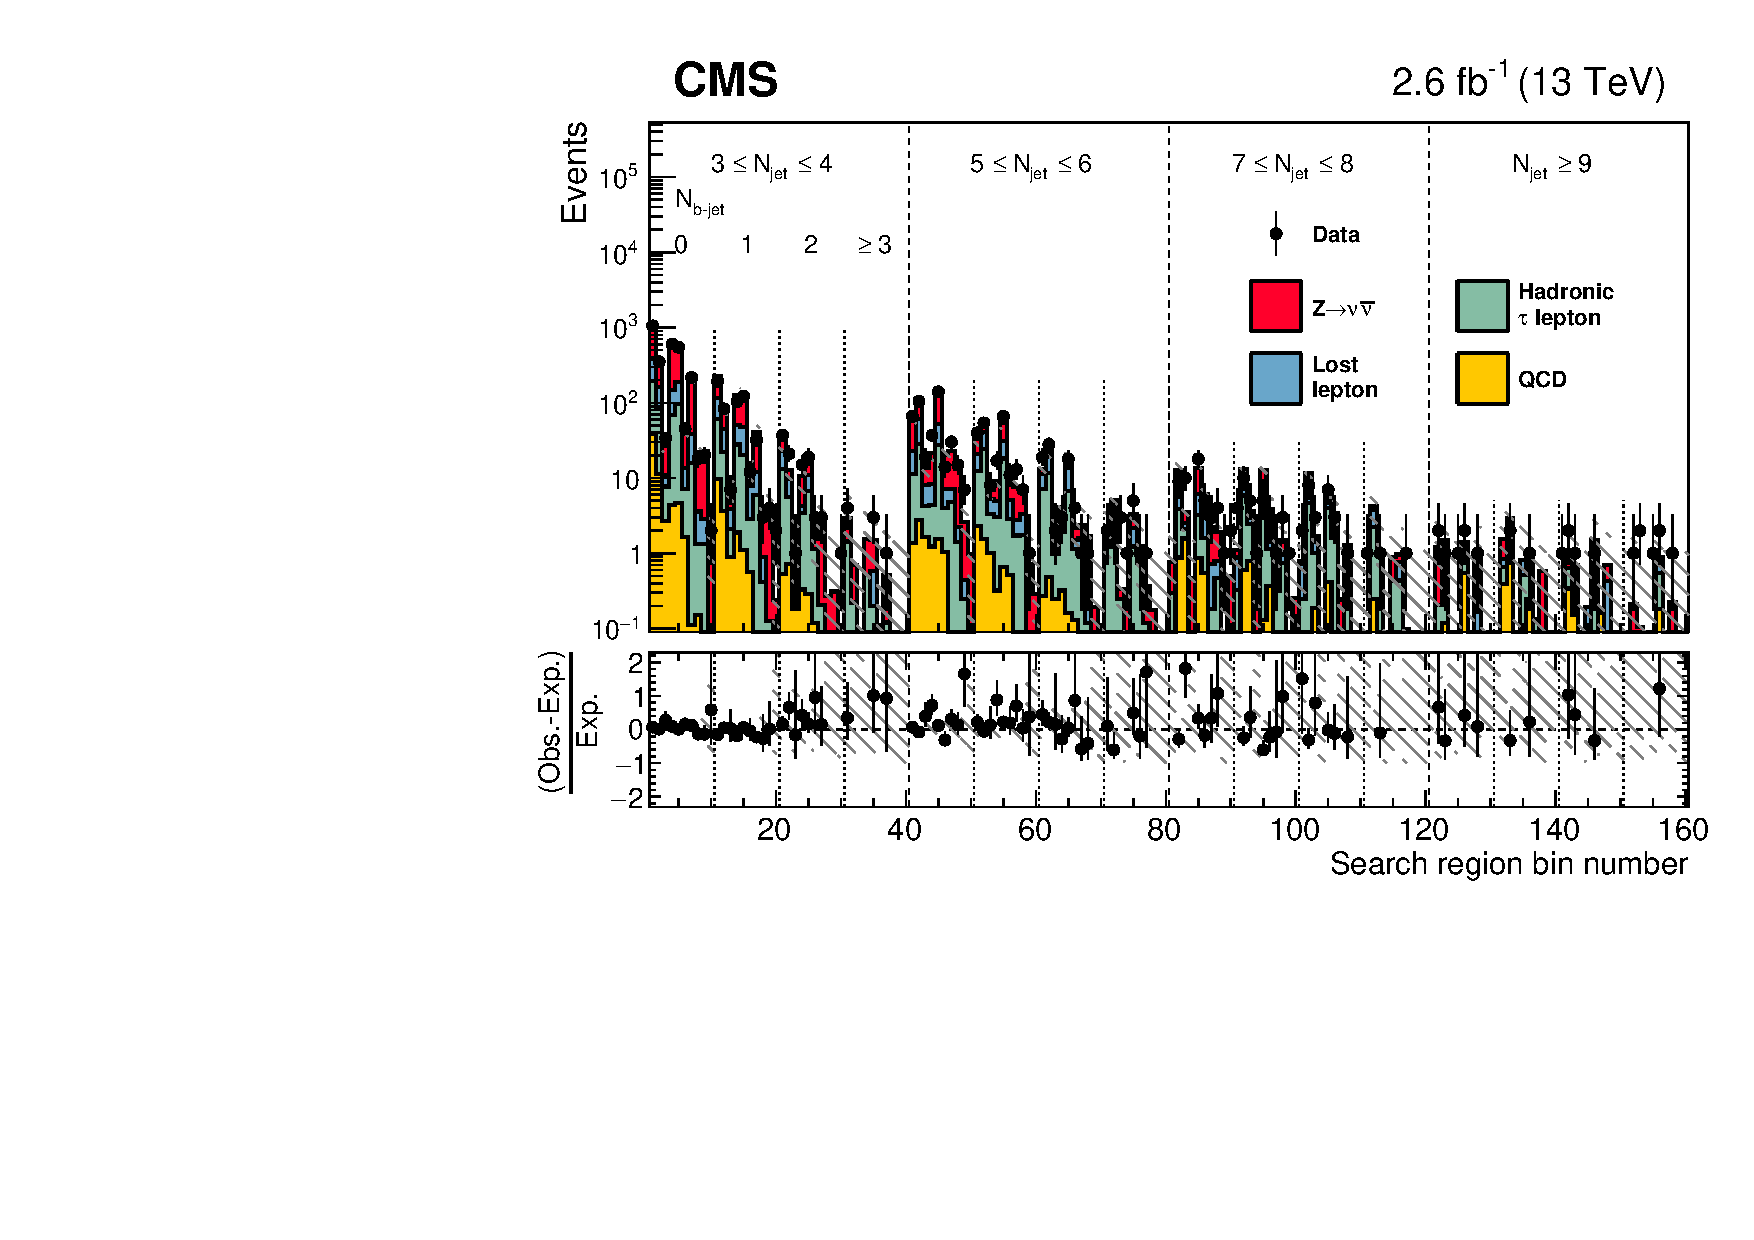
\includegraphics[width=15cm,height=10cm]{/home/bibhu/Desktop/PhDThesis/PhDThesis/chapter6/results2016prefit.pdf}
\caption{\label{fig:DataVsBkg2016} }
\end{figure}



\begin{figure}[h]
\centering
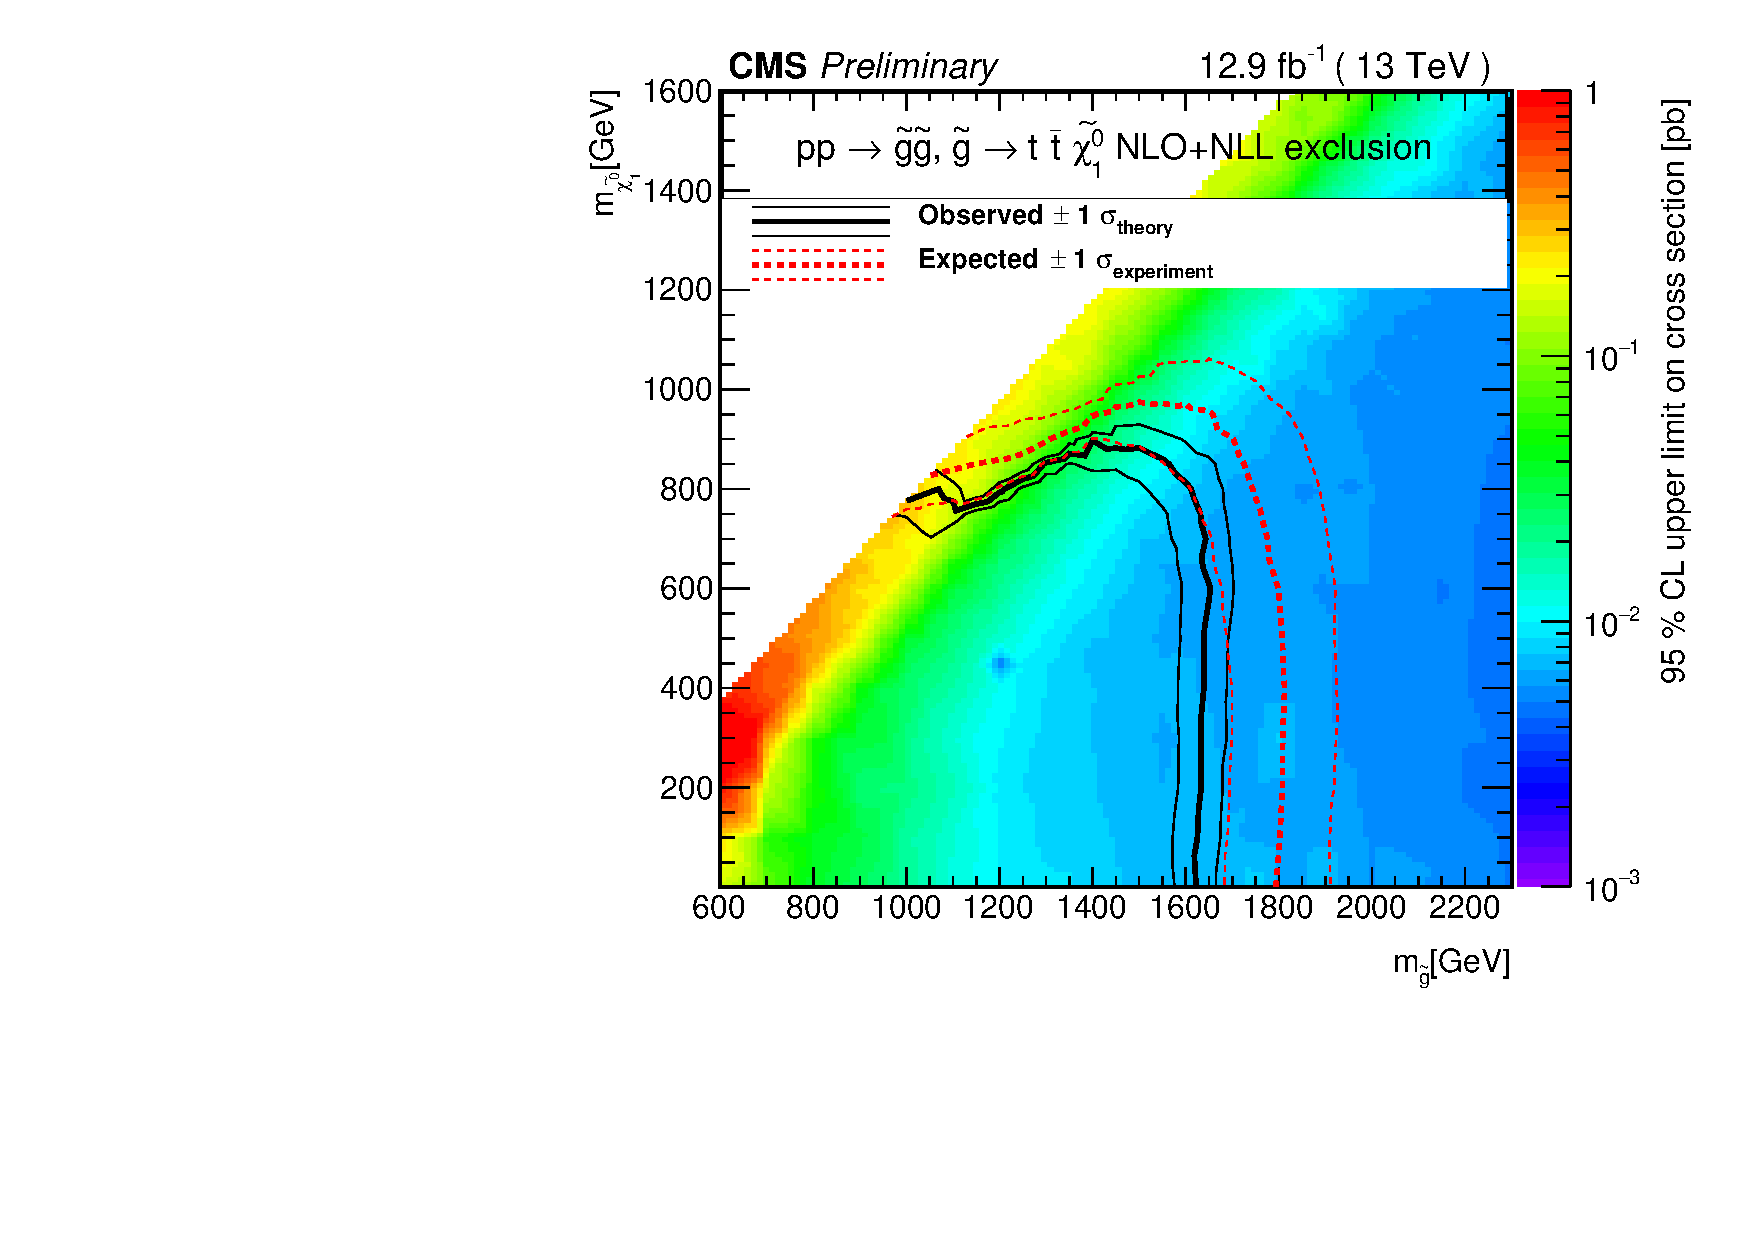
\includegraphics[width=0.32\textwidth]{/home/bibhu/Desktop/PhDThesis/PhDThesis/chapter6/T1tttt_12p9_limit.pdf}
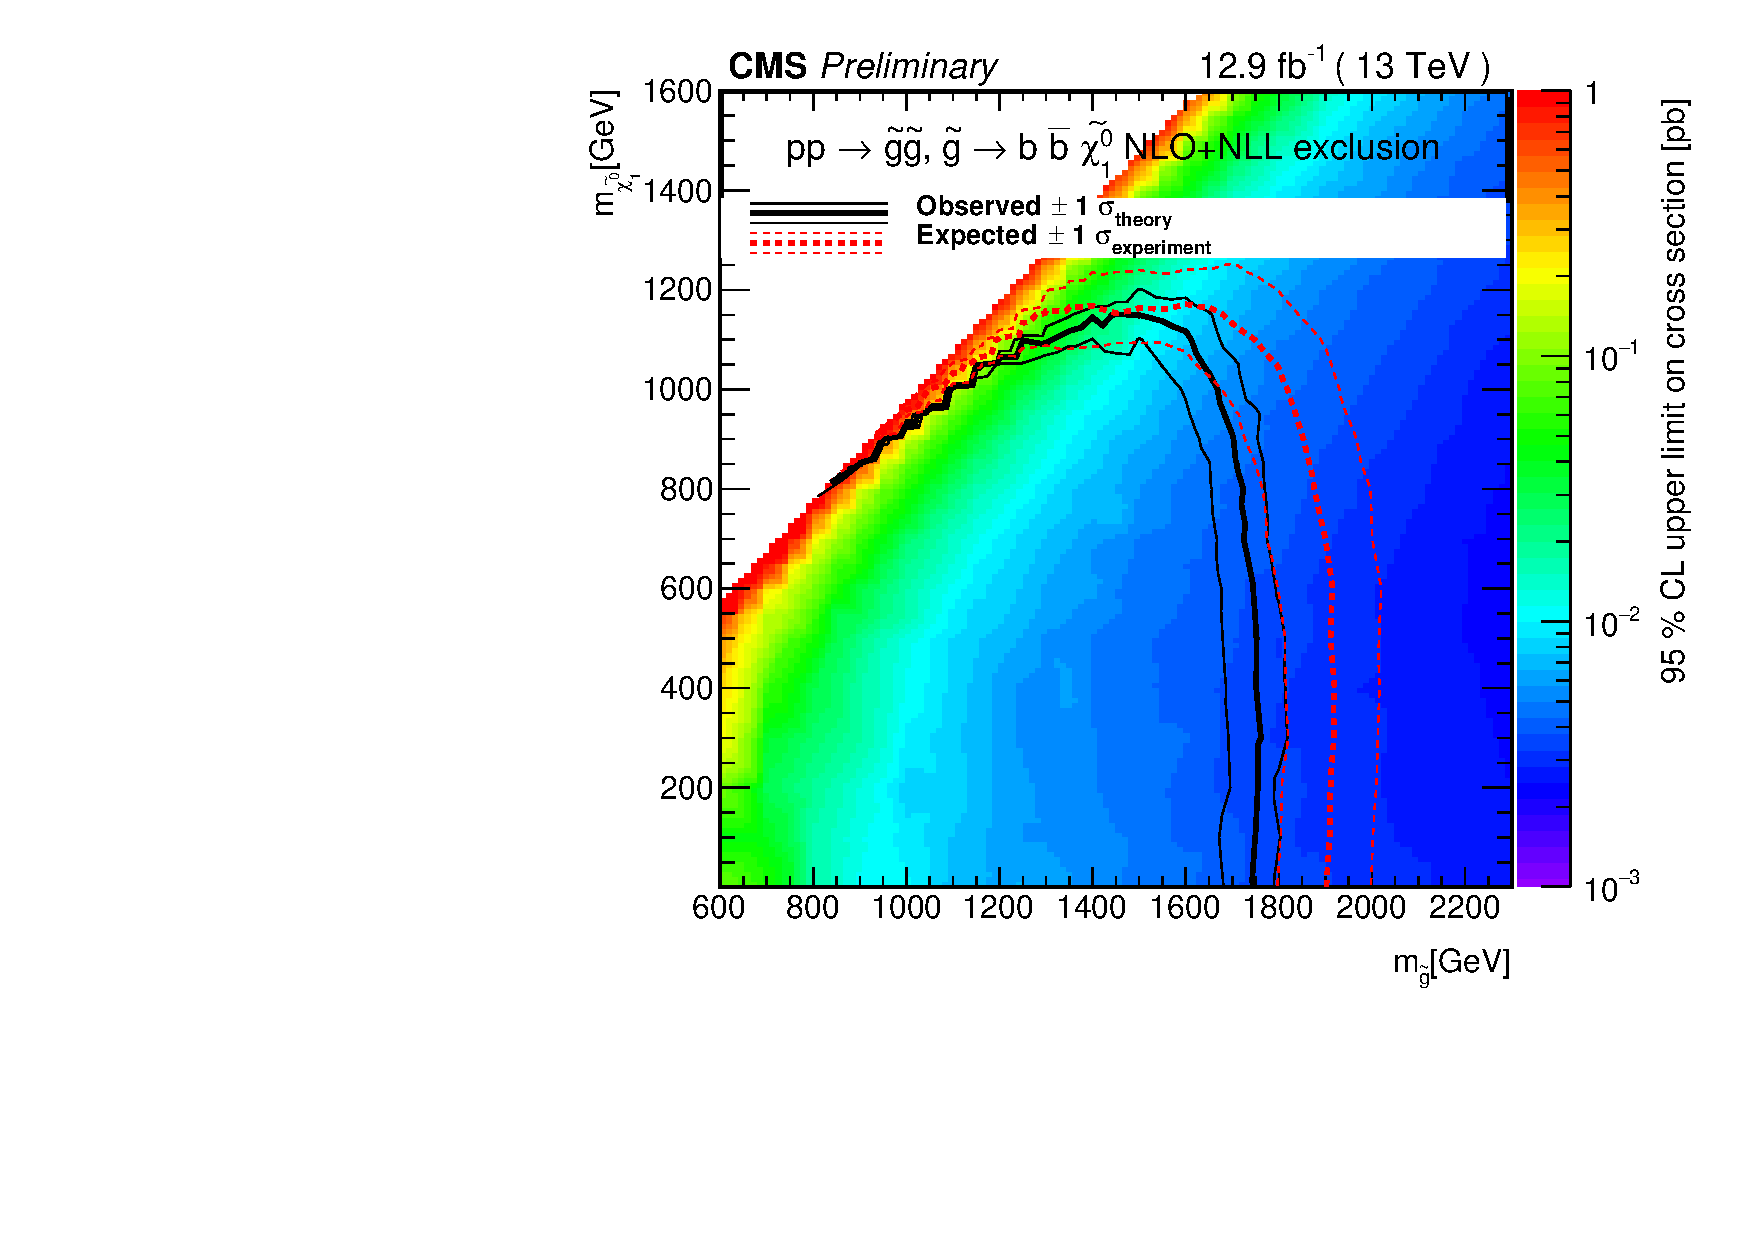
\includegraphics[width=0.32\textwidth]{/home/bibhu/Desktop/PhDThesis/PhDThesis/chapter6/T1bbbb_12p9_limit.pdf}
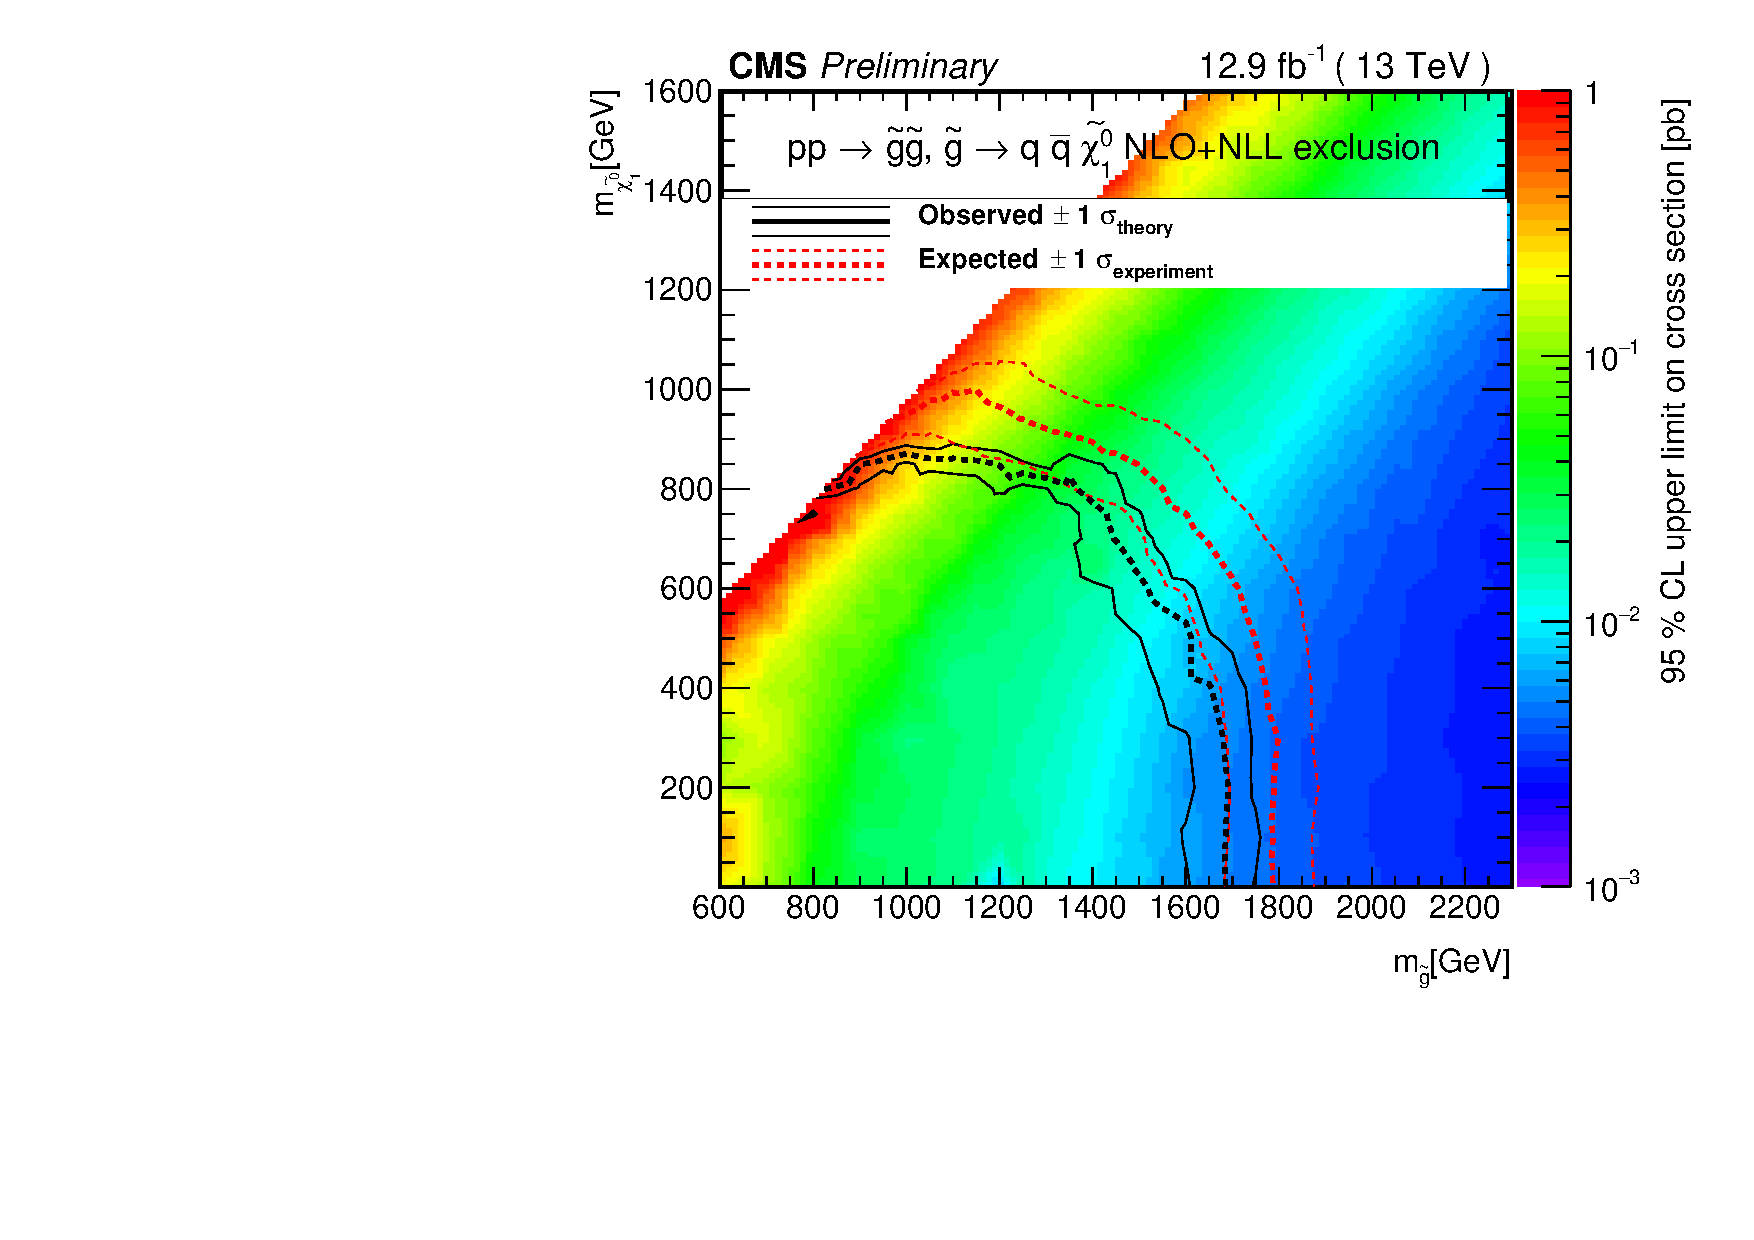
\includegraphics[width=0.32\textwidth]{/home/bibhu/Desktop/PhDThesis/PhDThesis/chapter6/T1qqqq_12p9_limit.pdf}
\caption{\label{fig:Limit2016}The 95\% CL upper limits on the production cross sections for four top quark (left),four light quark (middle) and four b-quark (right) in the final state. }
\end{figure}










